\documentclass[]{article}
\usepackage[margin=1in]{geometry}
\usepackage{amsthm}
\usepackage{mathtools}
\usepackage{amsfonts}
\usepackage{multicol}
\usepackage{tikz}
\usepackage{eurosym}
\usepackage{algorithm}
\usepackage{algorithmicx}
\usepackage{algpseudocode}
\DeclareRobustCommand{\officialeuro}{%
	\ifmmode\expandafter\text\fi
	{\fontencoding{U}\fontfamily{eurosym}\selectfont e}}
\usepackage{caption}
\usepackage{subcaption}
\usetikzlibrary{matrix}
\usepackage{ stmaryrd }
\newtheorem{definition}{Definition}[section]
\newtheorem{theorem}{Theorem}[section]
\newtheorem{lemma}[theorem]{Lemma}
\usepackage[toc,page]{appendix}
\usepackage{forest}



%opening
\title{Verifying Featured Transition Systems using Variability Parity Games}
\author{Sjef van Loo}

\begin{document}

\maketitle

\tableofcontents

\part{Verifying featured transition systems}
\label{part:verifying}
\section{Introduction}
Model verification techniques can be used to improve the quality of software. These techniques require the behaviour of the software to be modelled, after which the model can checked to verify that it behaves conforming to some requirement. Different languages are proposed and well studied to express these requirements, examples are LTL, CTL, CTL* and $\mu$-calculus (TODO: cite). Once the behaviour is modelled and the requirement is expressed in some language we can use modal checking techniques to determine if the model satisfies the requirement.

These techniques are well suited to model and verify the behaviour of a single software product. However software systems can be designed to have certain parts enabled or disabled. This gives rise to many software products that all behave very similar but not identical, such a collection is often called a \textit{product family}. The differences between the products in a product family is called the \textit{variability} of the family. A family can be verified by using the above mentioned techniques to verify every single product independently. However this approach does not use the similarities in behaviour of these different products, an approach that would make use of the similarities could potentially be a lot more efficient.

\textit{Labelled transition systems} (LTSs) are often used to model the behaviour of a system, while it can model behaviour well it cannot model variability. Efforts to also model variability include I/O automata, modal transition systems and \textit{featured transition systems} (FTSs) (TODO: cite). Specifically the latter is well suited to model all the different behaviours of the software products as well as the variability of the entire system in a single model.

Efforts have been made to verify requirements for entire FTSs, as well as to be able to reason about features. Notable contributions are fLTL, fCTL and fNuSMV (TODO: cite). However, as far as we know, there is no technique to verify an FTS against a $\mu$-calculus formula. Since the modal $\mu$-calculus is very expressive, it subsumes other temporal logics like LTL, CTL and CTL*, this is desired. In this thesis we will introduce a technique to do this. We first look at LTSs, the modal $\mu$-calculus and FTSs. Next we will look at an existing technique to verify an LTS, namely solving \textit{parity games}, as well as show how this technique can be used to verify an FTS by verifying every software product it describes independently. An extension to this technique is then proposed, namely solving \textit{variability parity games}. We will formally define variability parity games and prove that solving them can be used to verify FTSs.

\section{Verifying transition systems}
We first look at labelled transition systems (LTSs) and the modal $\mu$-calculus and what it means to verify an LTS. The definitions below are derived from \cite{Groote}.
\begin{definition}
	\label{def_lts}A labelled transition system (LTS) is a tuple $M = (S, Act, trans, s_0)$, where:
	\begin{itemize}
		\item $S$ is a set of states,
		\item $Act$ a set of actions,
		\item $trans \subseteq S \times Act \times S$ is the transition relation with $(s,a,s') \in trans$ denoted by $s \xrightarrow a s'$,
		\item $s_0 \in S$ is the initial state.
	\end{itemize}
\end{definition}
Consider the example in figure \ref{fig:coffeemachinebasiceurolts} (directly taken from \cite{FamBasedModelCheckingWithMCRL2}) of a coffee machine where we have two actions: ins (insert coin) and std (get standard sized coffee).\\
\begin{figure}[h]
	\centering
	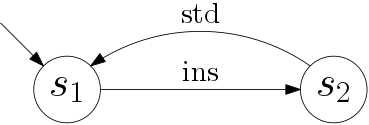
\includegraphics[scale=0.3]{Examples/CoffeeMachine/BasicEuroLTS}
	\caption[Coffee machine LTS]{Coffee machine LTS $C$}
	\label{fig:coffeemachinebasiceurolts}
\end{figure}


\begin{definition}
	\label{def_mu_syntax}
	A modal $\mu$-calculus formula over the set of actions $Act$ and a set of variables $\mathcal{X}$ is defined by
	\[ \varphi = \top\ |\ \bot\ |\ X\ |\ \varphi \vee \varphi\ |\ \varphi \wedge \varphi\ |\ \langle a \rangle \varphi\ |\ [a]\varphi\ |\ \mu X.\varphi\ |\ \nu X.\varphi \]
	with $a \in Act$ and $X \in \mathcal{X}$. 
	
	
	No negations in the language because negations can be pushed inside to the propositions, ie. the $\top$ and $\bot$ elements.
\end{definition}
The modal $\mu$-calculus contains boolean constants $\top$ and $\bot$, propositional operators $\vee$ and $\wedge$, modal operators $\langle \, \rangle$ and $[ \, ]$ and fixpoint operators $\mu$ and $\nu$. A formula is closed when variables only occur in the scope of a fixpoint operator for that variable.

A modal $\mu$-calculus formula can be interpreted with an LTS, this results in a set of states for which the formula holds.
\begin{definition}
	\label{def_mu_sem} For LTS $(S, Act, trans, s_0)$ we inductively define the interpretation of a modal $\mu$-calculus formula $\varphi$, notation
	$[\![ \varphi ]\!]^\eta$, where $\eta : \mathcal{X} \rightarrow \mathcal{P}(S)$ is a logical variable valuation, as a set of states
	where $\varphi$ is valid, by:
	\begin{align*}
	&[\![ \mathit{\top} ]\!]^\eta &&= S\\
	&[\![ \mathit{\bot} ]\!]^\eta &&= \emptyset\\
	&[\![ \varphi_1 \wedge \varphi_2 ]\!]^\eta &&= [\![ \varphi_1 ]\!]^\eta \cap [\![ \varphi_2 ]\!]^\eta \\
	&[\![ \varphi_1 \vee \varphi_2 ]\!]^\eta &&= [\![ \varphi_1 ]\!]^\eta \cup [\![ \varphi_2 ]\!]^\eta\\
	&[\![ \langle a \rangle \varphi ]\!]^\eta &&= \{s \in S|\exists_{s' \in S} s \xrightarrow {a} s' \wedge s' \in [\![ \varphi ]\!]^\eta\}\\
	&[\![ [ a ] \varphi ]\!]^\eta &&= \{s \in S|\forall_{s' \in S} s \xrightarrow {a} s' \implies s' \in [\![ \varphi ]\!]^\eta\}\\
	&[\![ \mu X. \varphi ]\!]^\eta &&= \bigcap_{f \subseteq S}\{f | f = [\![ \varphi ]\!]^{\eta[X:=f]}\}\\
	&[\![ \nu X. \varphi ]\!]^\eta &&= \bigcup_{f \subseteq S}\{f | f = [\![ \varphi ]\!]^{\eta[X:=f]}\}\\
	&[\![ X ]\!]^\eta &&= \eta(X)
	\end{align*}
\end{definition}

Given closed formula $\varphi$, LTS $M = (S, Act, trans, s_0)$ and $s \in S$ we write $(M,s) \models \varphi$ iff $s \in [\![ \varphi ]\!]^\eta$ for $M$, we say that formula $\varphi$ holds for $M$ in state $s$. If formula $\varphi$ holds for $M$ in the initial state we say that formula $\varphi$ holds for $M$ and write $M \models \varphi$.

Again consider the coffee machine example (figure \ref{fig:coffeemachinebasiceurolts}) and formula $\varphi = \nu X. \mu Y. ([ins]Y \wedge [std] X)$ (taken from \cite{FamBasedModelCheckingWithMCRL2}) which states that action \textit{std} must occur infinitely often over all runs. Obviously this holds for the coffee machine, therefore we have $C \models \varphi$.

\subsection{Featured transition systems}
A \textit{featured transition system} (FTS) extends the LTS definition to express variability. It does so by introducing \textit{features} and \textit{products} into the definition. Features are options that can be enabled or disabled for the system. A product is a feature assignments, ie. a set of features that is enabled for that product. Not all products are valid, some features might be mutually exclusive and some features might always be required. To express the relation between features one can use feature diagrams as explained in \cite{Classen2013FeaturedTS}. Feature diagrams offer a nice way of expressing which feature assignments are valid, however for simplicity we will represent the collection of valid products simply with a set of feature assignments. Finally FTSs guard every transition with a boolean expression over the set of features. We have the following definition, based on \cite{Classen2013FeaturedTS}:
\begin{definition}
	\label{def_fts}A featured transition system (FTS) is a tuple $M = (S, Act, trans, s_0, N, P, \gamma)$, where:
	\begin{itemize}
		\item $S, Act, trans, s_0$ are defined as in an LTS,
		\item $N$ is a non-empty set of features,
		\item $P \subseteq \mathcal{P}(N)$ is a set of products, ie. feature assignments, that are valid,
		\item $\gamma : trans \rightarrow \mathbb{B}(N)$ is a total function, labelling each transition with a boolean expression over the features. A product $p \in \mathcal{P}(N)$ satisfying the boolean expression of transition $t$ is denoted by $p \models \gamma(t)$. The boolean expression that is satisfied by any feature assignment is denoted by $\top$, ie $p \models \top$ for any $p$.
		
		A transition $s \xrightarrow a s'$ and $\gamma((s,a,s')) = f$ is denoted by $s \xrightarrow {a | f} s'$. 
	\end{itemize}
\end{definition}
\begin{figure}[h]
\centering
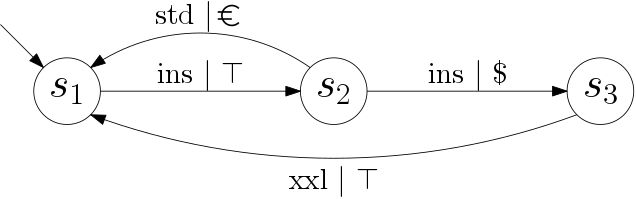
\includegraphics[scale=0.3]{Examples/CoffeeMachine/FTS}
\caption[Coffee machine LTS]{Coffee machine FTS $C$}
\label{fig:coffeemachinefts}
\end{figure}

Consider the example in figure \ref{fig:coffeemachinefts} (directly taken from \cite{FamBasedModelCheckingWithMCRL2}) which shows an FTS for a coffee machine For this example we have two features $N = \{\$, \officialeuro\}$ and two valid products $P = \{\{\$\},\{\officialeuro\}\}$.

An FTS expresses the behaviour of multiple products, we can derive the behaviour of a single product by simply removing all the transitions from the FTS for which the product doesn't satisfy the feature expression guarding the transition. We call this a \textit{projection} \cite{Classen2013FeaturedTS}.

\begin{definition}
	\label{def_fts_proj}
	The projection of an FTS $M = (S, Act, trans, s_0, N, P, \gamma)$ to a product $p \in P$, noted $M_{|p}$, is the LTS $M'=(S,Act,trans', s_0)$, where $trans' = \{t \in trans\ |\ p \models \gamma(t)\}$.
\end{definition}
The coffee machine example can be projected to its two products, which results in the LTSs in figure \ref{fig:cofeemachineftsproj}.
\begin{figure}[h]
	\centering
	\begin{subfigure}{.5\textwidth}
		\centering
		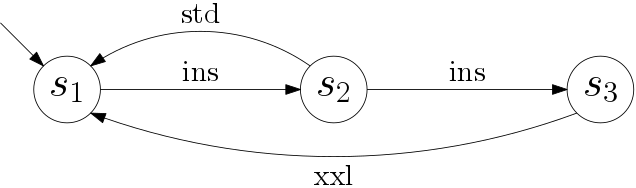
\includegraphics[width=1\linewidth]{Examples/CoffeeMachine/FTSProjDollar}
		\caption[$C_{|\{\$\}}$]{$C$ projected to the dollar product: $C_{|\{\$\}}$}
		\label{fig:coffeemachineftsprojdollar}
	\end{subfigure}%
	\begin{subfigure}{.5\textwidth}
		\centering
		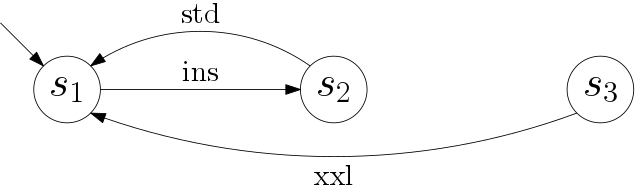
\includegraphics[width=1\linewidth]{Examples/CoffeeMachine/FTSProjEuro}
		\caption[$C_{|\{\$\}}$]{$C$ projected to the euro product: $C_{|\{\officialeuro\}}$}
		\label{fig:coffeemachineftsprojeuro}
	\end{subfigure}
	\caption{Projections of the coffee machine FTS}
	\label{fig:cofeemachineftsproj}
\end{figure}
\subsection{FTS verification question}
When verifiying an FTS against a model $\mu$-calculus formula $\varphi$, we are trying to answer the question: For which products in the FTS does its projection satisfy $\varphi$? Formally, given FTS $M = (S, Act, trans, s_0, N, P, \gamma)$ and modal $\mu$-calculus formula $\varphi$ we want to find $P_s \subseteq P$ such that:
\begin{itemize}
	\item for every $p \in P_s$ we have $M_{|p} \models \varphi$ and
	\item for every $p \in P \backslash P_s$ we have $M_{|p} \not\models \varphi$.
\end{itemize}
Furthermore a counterexample for every $p \in P \backslash P_s$ is preferred.

\section{Verification using parity games}
Verifying LTSs against a modal $\mu$-calculus formula can be done by solving a \textit{parity game}. This is done by translating an LTS in combination with a formula to a parity game, the solution of the parity game provides the information needed to conclude if the model satisfies the formula. This relation is depicted in figure \ref{fig:ltsverificationusingpg}. This technique is well known and well studied, in this section we will first look at parity games, the translation from LTS and formula to a parity game and finally what we can do with this technique to verify FTS.
\begin{figure}[h]
	\centering
	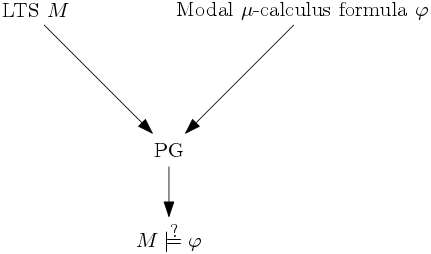
\includegraphics[scale=0.5]{Diagrams/LTSVerificationUsingPG}
	\caption[LTS verification using PG]{LTS verification using PG}
	\label{fig:ltsverificationusingpg}
\end{figure}


\subsubsection{Parity games}
\begin{definition}
	\label{def_PG}\cite{Bradfield2018}
	A parity game (PG) is a tuple $(V, V_0, V_1, E, \Omega)$, where:
	\begin{itemize}
		\item $V = V_0 \cup V_1$ and $V_0 \cap V_1 = \emptyset$,
		\item $V_0$ is the set of vertices owned by player $0$,
		\item $V_1$ is the set of vertices owned by player $1$, 
		\item $E \subseteq V \times V$ is the edge relation,
		\item $\Omega :  V \rightarrow \mathbb{N}$ is a priority assignment.
	\end{itemize}
\end{definition}
A parity game is played by players 0 and 1. We write $\alpha \in \{0,1\}$ to denote an arbitrary player. We write $\overline{\alpha}$ to denote $\alpha$'s opponent, ie. $\overline{0} = 1$ and $\overline{1} = 0$.

 A play starts with placing a token on vertex $v \in V$. Player $\alpha$ moves the token if the token is on a vertex owned by $\alpha$, ie. $v \in V_\alpha$. The token can be moved to $w \in V$, with $(v,w) \in E$. A series of moves results in a sequence of vertices, called a path. For path $\pi$ we write $\pi_i$ to denote the $i^{\text{th}}$ vertex in path $\pi$. A play ends when the token is on vertex $v \in V_\alpha$ and $\alpha$ can't move the token anywhere, in this case player $\overline{\alpha}$ wins the play. If the play results in an infinite path $\pi$ then we determine the highest priority that occurs infinitely often in this path, formally
\[ \max\{ p \ |\ \forall_j \exists_i j < i \wedge p = \Omega(\pi_i) \}\] 
If the highest priority is odd then player $1$ wins, if it is even player $0$ wins.
\begin{figure}[h]
	\centering
	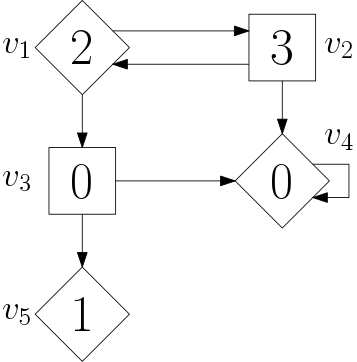
\includegraphics[scale=0.3]{Examples/SimplePG/PG}
	\caption[Parity game example]{Parity game example}
	\label{fig:simplepgpg}
\end{figure}

Figure \ref{fig:simplepgpg} shows an example of a parity game. We usually depict the vertices owned by player $0$ by diamonds and vertices owned by player $1$ by boxes, the priority is depicted inside the vertices. If the game starts by placing a token on $v_1$ we can consider the following exemplary paths:
\begin{itemize}
	\item $\pi = v_1v_3v_5$ is won by player $1$ since player $0$ can't move at $v_5$.
	\item $\pi = (v_1v_2)^\omega$ is won by player $1$ since the highest priority occurring infinitely often is 3.
	\item $\pi = v_1v_3(v_4)^\omega$ is won by player $0$ since the highest priority occurring infinitely often is $0$.
\end{itemize}


A strategy for player $\alpha$ is a function $\sigma : V^*V_\alpha \rightarrow V$ that maps a path ending in a vertex owned by player $\alpha$ to the next vertex. Parity games are positionally determined \cite{Bradfield2018}, therefore a strategy $\sigma: V_\alpha \rightarrow V$ that maps the current vertex to the next vertex is sufficient. 

A strategy $\sigma$ for player $\alpha$ is winning from vertex $v$ iff any play that results from following $\sigma$ results in a win for player $\alpha$. The graph can be divided in two partitions $W_0 \subseteq V$ and $W_1 \subseteq V$, called winning sets. Iff $v \in W_\alpha$ then player $\alpha$ has a winnings strategy from $v$. Every vertex in the graph is either in $W_0$ or $W_1$ \cite{Bradfield2018}. Furthermore finite parity games are decidable \cite{Bradfield2018}.


\subsubsection{Creating parity games}
A parity game can be created from a combination of an LTS and a modal $\mu$-calculus formula. To do this we introduce some auxiliary definitions regarding the modal $\mu$-calculus.

First we introduce the notion of unfolding, a fixpoint formula $\mu X . \varphi$ can be unfolded resulting in formula $\varphi$ where every occurrence of $X$ is replaced by $\mu X . \varphi$, denoted by $\varphi [ X:= \mu X . \varphi]$. A fixpoint formula is equivalent to its unfolding \cite{Bradfield2018}, ie. for some LTS $[\![\mu X . \varphi]\!]^\eta = [\![\varphi[X:=\mu X . \varphi]]\!]^\eta$. The same holds for the fixpoint operator $\nu$.

Next we define the Fischer-Ladner closure for a closed $\mu$-calculus formula 
\cite{STREETT1989249,FISCHER1979194}. The Fischer-Ladner closure of $\varphi$ is the set $\textit{FL}(\varphi)$ of closed formula's containing at least $\varphi$. Furthermore for every formula $\psi$ in $\textit{FL}(\varphi)$ it holds that for every direct subformula $\psi'$ of $\psi$ there is a formula in $\textit{FL}(\varphi)$ that is equivalent to $\psi'$.
\begin{definition}
	\label{def_FLClosure}
	The Fischer-Ladner closure of closed $\mu$-calculus formula $\varphi$ is the smallest set $\textit{FL}(\varphi)$ satisfying the following constraints:
	\begin{itemize}
		\item $\varphi \in \textit{FL}(\varphi)$,
		\item if $\varphi_1 \vee \varphi_2 \in \textit{FL}(\varphi)$ then $\varphi_1 ,\varphi_2 \in \textit{FL}(\varphi)$,
		\item if $\varphi_1 \wedge \varphi_2 \in \textit{FL}(\varphi)$ then $\varphi_1 ,\varphi_2 \in \textit{FL}(\varphi)$,
		\item if $\langle a \rangle \varphi' \in \textit{FL}(\varphi)$ then $\varphi' \in \textit{FL}(\varphi)$,
		\item if $[ a ] \varphi' \in \textit{FL}(\varphi)$ then $\varphi' \in \textit{FL}(\varphi)$,
		\item if $\mu X . \varphi' \in \textit{FL}(\varphi)$ then $\varphi'[X:= \mu X . \varphi'] \in \textit{FL}(\varphi)$ and
		\item if $\nu X . \varphi' \in \textit{FL}(\varphi)$ then $\varphi'[X:= \nu X . \varphi'] \in \textit{FL}(\varphi)$.
		
	\end{itemize}
\end{definition}

Finally we define alternating depth.
\begin{definition}\cite{Bradfield2018}
	The dependency order on bound variables of $\varphi$	is the smallest partial order such that $X \leq_\varphi Y$ if $X$ occurs free in $\sigma Y. \psi$ . The alternation depth of a $\mu$-variable X in formula $\varphi $ is the maximal length of a chain $X_1 \leq_\varphi  \dots \leq_\varphi X_n$ where $X = X_1$, variables $X_1, X_3, \dots$ are $\mu$-variables and variables $X_2, X_4, \dots$ are $\nu$-variables. The alternation depth of a $\nu$-variable is defined similarly. The alternation depth of formula $\varphi$, denoted $adepth(\varphi)$, is the maximum of the alternation depths of the variables bound in $\varphi$, or zero if there are no fixpoints.
\end{definition}
Consider the example formula $\varphi = \nu X. \mu Y. ([ins]Y \wedge [std] X)$ which states that for an LTS with $Act = \{ ins, std\}$ the action \textit{std} must occur infinitely often over all runs. Since $X$ occurs free in $\mu Y. ([ins] Y \wedge [std]X)$ we have $adepth(Y) = 1$ and $adepth(X) = 2$. As shown in \cite{Bradfield2018} it holds that formula $\mu X. \psi$ has the same alternation depth as its unfolding $\psi[X:=\mu X. \psi]$. Similarly for the greatest fixpoint.



We can now define the transformation from an LTS and a formula to a parity game.
\begin{definition}
	\label{def_LTS2PG}\cite{Bradfield2018}
	LTS2PG($M, \varphi$) converts LTS $M = (S, Act, trans, s_0)$ and closed formula $\varphi$ to a PG $(V, V_0, V_1, E, \Omega)$.
	
	A vertex in the parity game is represented by a pair $(s, \psi)$ where $s \in S$ and $\psi$ is a modal $\mu$-calculus formula. We will create a vertex for every state with every formula in the Fischer-Ladner closure of $\varphi$. We define the set of vertices:
	\[ V = S \times \textit{FL}(\varphi) \]
	
	We create the parity game with the smallest set $E$ such that:
	\begin{itemize}
		\item $V = V_0 \cup V_1$,
		\item $V_0 \cap V_1 = \emptyset$ and
		\item for every $v = (s, \psi) \in V$ we have:
		\begin{itemize}
			\item If $\psi = \top$ then $v \in V_1$.
			\item If $\psi = \bot$ then $v \in V_0$.
			\item If $\psi = \psi_1 \vee \psi_2$ then:
			\subitem $v \in V_0$,
			\subitem $(v, (s,\psi_1)) \in E$ and
			\subitem $(v, (s,\psi_2)) \in E$.
			\item If $\psi = \psi_1 \wedge \psi_2$ then:
			\subitem $v \in V_1$,
			\subitem $(v, (s,\psi_1)) \in E$ and
			\subitem $(v, (s,\psi_2)) \in E$.
			\item If $\psi = \langle a \rangle \psi'$ then $v \in V_0$ and for every $s \xrightarrow{ a} s'$ we have $(v, (s', \psi')) \in E$.
			\item If $\psi = [ a ] \psi'$ then $v \in V_1$ and for every $s \xrightarrow{ a} s'$ we have  $(v, (s', \psi')) \in E$.
			\item If $\psi = \mu X. \psi'$ then $(v, (s, \psi'[X:=\mu X. \psi'])) \in E$.
			\item If $\psi = \nu X. \psi'$ then $(v, (s, \psi'[X:=\nu X. \psi'])) \in E$.
		\end{itemize}
	\end{itemize}
	Since the Fischer-Ladner formula's are closed we never get the case $\psi = X$.
	
	Finally we have $\Omega(s, \psi) = \begin{cases}
	2 \lfloor adepth(X) / 2 \rfloor & \text{if } \psi = \nu X. \psi'\\
	2 \lfloor adepth(X) / 2 \rfloor + 1 & \text{if } \psi = \mu X. \psi'\\
	0 & \text{otherwise}
	\end{cases}$
\end{definition}
\begin{figure}[h]
	\centering
	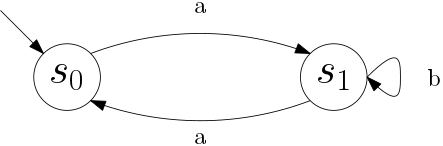
\includegraphics[scale=0.3]{Examples/ExamleVerification/LTSprojempty}
	\caption[LTS $M$]{LTS $M$}
	\label{fig:exverltsprojempty}
\end{figure}\begin{figure}[h]
\centering
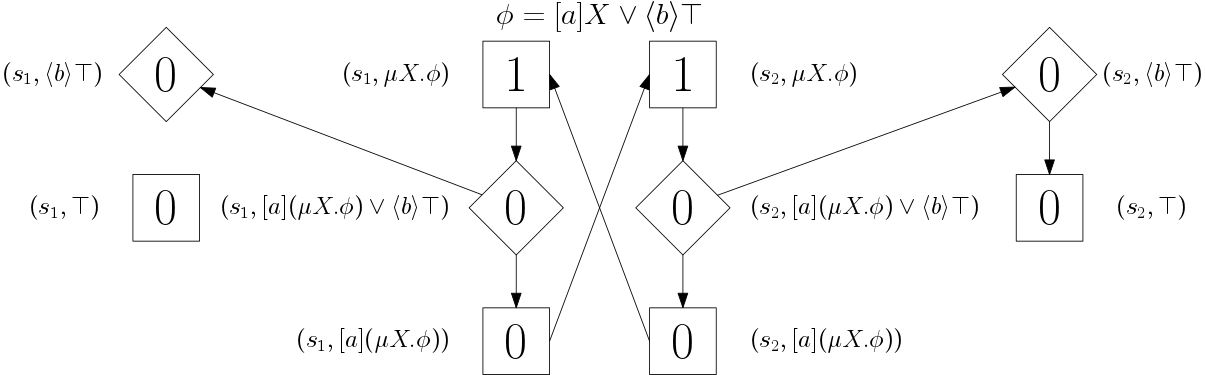
\includegraphics[scale=0.3]{Examples/ExamleVerification/PG}
\caption[Parity game $LTS2PG(M, \varphi)$]{Parity game $LTS2PG(M, \varphi)$}
\label{fig:exverpg}
\end{figure}
Consider LTS $M$ in figure \ref{fig:exverltsprojempty} and formula $\varphi = \mu X.([a]X \vee \langle b \rangle \top)$ expressing that on any path reached by $a$'s we can eventually do a $b$ action. We will use this as a working example in the next few sections. The resulting parity game is depicted in figure \ref{fig:exverpg}. Solving this parity game results in the following winning sets:%
\begin{align*}
	W_0 = \{& (s_1, \mu X.\phi),\\
	& (s_1, [a](\mu X. \phi) \vee \langle b \rangle \top),\\
	& (s_1, [a](\mu X. \phi)),\\
	& (s_1, \top),\\
	& (s_2, \mu X.\phi),\\
	& (s_2, [a](\mu X. \phi) \vee \langle b \rangle \top),\\
	& (s_2, [a](\mu X. \phi)),\\
	& (s_2, \langle b \rangle \top),\\
	& (s_2, \top)
	\}\\
	W_1 = \{& (s_1, \langle b \rangle \top )\}
\end{align*}
With the strategies $\sigma_0$ for player $0$ and $\sigma_1$ for player $1$ being (vertices with one outgoing edge are omitted):
\begin{align*}
\sigma_0 = \{
&(s_1, [a](\mu X. \phi) \vee \langle b \rangle \top) \mapsto (s_1, [a] (\mu X. \phi)), \\
&(s_2, [a](\mu X. \phi) \vee \langle b \rangle \top) \mapsto (s_2, \langle b \rangle \top) \} \\
\sigma_1 = \{&\} \\
\end{align*}

State $s$ in LTS $M$ only satisfies $\varphi$ iff player $0$ has a winning strategy from vertex $(s, \varphi)$. This is formally stated in the following theorem which is proven in \cite{Bradfield2018}.
\begin{theorem}
	\label{the_LTS_PG_REL}Given LTS $M = (S, Act, trans, s_0)$, modal $\mu$-calculus formula $\varphi$ and state $s \in S$ it holds that $(M, s) \models \varphi$ iff $s \in W_0$ for the game $LTS2PG(M, \varphi)$.
\end{theorem}

\subsubsection{FTSs and parity games}
Using the theory we have seen thus far we can verify FTSs by verifying every projection of the FTS to a valid product. This relation is depicted in the following diagram where $\Pi$ indicates a projection:
\\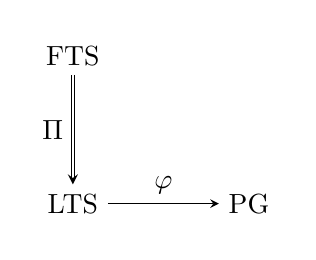
\begin{tikzpicture}
\matrix (m) [matrix of math nodes,row sep=4em,column sep=4em,minimum width=2em]
{
	\text{FTS} \\
	\text{LTS} & \text{PG} \\};
\path[-stealth]
(m-1-1) edge [double] node [left] {$\Pi$} (m-2-1)
(m-2-1.east|-m-2-2) edge node [above] {$\varphi$}
(m-2-2)
;
\end{tikzpicture}\\
As mentioned before verifying products dependently is potentially more efficient. In the next two sections we define an extension to parity games, namely \textit{variability parity games} (VPGs) which can be used to verify an FTS. We will translate an FTS and a formula into a VPG which solution will provide the information needed to conclude for which products the FTS satisfies the formula.


\section{Featured parity games}
Before we can define variability parity games we first define \textit{featured parity games} (FPG), featured parity games extend the definition of parity games to capture the variability represented in an FTS. It uses the same concepts as FTSs: features, products and a function that guards edges. In this section we will introduce the definition of FPGs and show that solving them answers the verification questions for FTS: For which products in the FTS does its projection satisfy $\varphi$?

First we introduce the definition of an FPG:
\begin{definition}
	\label{def_FPG}
	A featured parity game (FPG) is a tuple $(V,V_0, V_1, E, \rho, N, P, \gamma)$, where:
	\begin{itemize}
		\item $V = V_0 \cup V_1$ and $V_0 \cap V_1 = \emptyset$,
		\item $V_0$ is the set of vertices owned by player $0$,
		\item $V_1$ is the set of vertices owned by player $1$, 
		\item $E \subseteq V \times V$ is the edge relation,
		\item $\rho :  V \rightarrow \mathbb{N}$ is a priority assignment,
		\item $N$ is a set of features,
		\item $P \subseteq \mathcal{P}(N)$ is a set of products, ie. feature assignments, for which the game can be played,
		\item $\gamma : E \rightarrow \mathbb{B}(N)$ is a total function, labelling each edge with a Boolean expression over the features.
	\end{itemize}
\end{definition}
An FPG is played similarly to a PG, however the game is played for a specific product $p \in P$. Player $\alpha$ can only move the token from $v \in V_\alpha$ to $w \in V$ if $(v,w) \in E$ and $p \models \gamma(v,w)$.

A game played for product $p \in P$ results in winnings sets $W_0^p$ and $W_1^p$, which are defined similar to the $W_0$ and $W_1$ winning sets for parity games.

An FPG can simply be projected to a product $p$ by removing the edges that are not satisfied by $p$.
\begin{definition}
	\label{def_FPG_proj}
The projection from FPG $G = (V,V_0, V_1, E, \rho, N, P, \gamma)$ to a product $p \in P$, noted $G_{|p}$, is the parity game $(V,V_0,V_1, E', \rho)$ where $E' = \{ e \in E\ |\ p \models \gamma(e) \}$.
\end{definition}

Playing FPG $G$ for a specific product $p\in P$ is the same as playing the PG $G_{|p}$. Any path that is valid in $G$ for $p$ is also valid in $G_{|p}$ and vice versa. Therefore the strategies are also interchangeable, furthermore the winning sets $W_\alpha$ for $G_{|p}$ and $W_\alpha^p$ for $G$ are identical. Since parity games are positionally determined so are FPGs. Similarly, since finite parity games are decidable, so are finite FPGs.

Solving an FPG means determining winning sets for every valid product in the FPG.
\subsection{Creating featured parity games}
An FPG can be created from an FTS in combination with a model $\mu$-calculus formula. We translate an FTS to an FPG by first creating a PG from the transition system as if there were no transition guards, next we apply the same guards to the FPG as are present in the FTS for edges that originate from transitions. The features and valid products in the FPG are identical to those in the FTS.
\begin{definition}
	\label{def_FTS2FPG}
	$FTS2FPG(M, \varphi)$ converts FTS $M = (S, Act, trans, s_0, N, P, \gamma)$ and closed formula $\varphi$ to FPG $(V, V_0, V_1, E, \rho, N, P, \gamma')$.
	
	We have $(V, V_0, V_1, E, \rho)$ = LTS2PG($(S, Act, trans, s_0), \varphi$) and
	\[ \gamma'((s, \psi),(s', \psi')) = \begin{cases}
	\gamma(s,a,s') & \text{if }\psi = \langle a \rangle \psi'\text{ or }\psi = [a]\psi' \\
	\top & \text{otherwise}
	\end{cases}\]
\end{definition}
Consider our working example which we extend to an FTS depicted in figure \ref{fig:exverfts}, for this example we have features $N = \{f, g\}$ and products $P = \{\emptyset, \{f\},\{f,g\}\}$.
\begin{figure}[h]
	\centering
	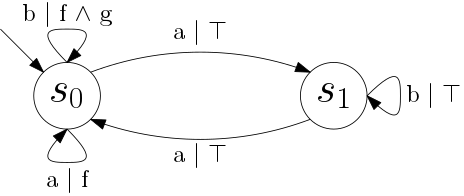
\includegraphics[scale=0.3]{Examples/ExamleVerification/FTS}
	\caption[FTS $M$]{FTS $M$}
	\label{fig:exverfts}
\end{figure}
\begin{figure}[h]
	\centering
	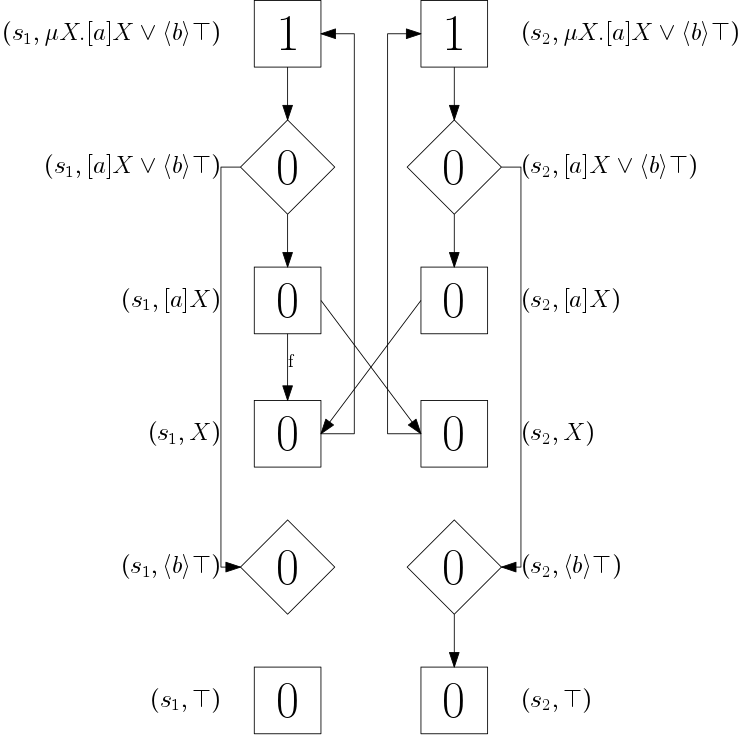
\includegraphics[scale=0.3]{Examples/ExamleVerification/FPG}
	\caption[FPG for $M$ and $\varphi$]{FPG for $M$ and $\varphi$}
	\label{fig:exverfpg}
\end{figure}
We can translate this FTS with formula $\varphi = \mu X. ([a] X \vee \langle b \rangle \top)$ to an FPG depicted in figure \ref{fig:exverfpg}. As we can see from the FTS if feature $f$ is enabled and $g$ is disabled then we have an infinite path of $a$'s where $b$ is never enabled, therefore $\varphi$ doesn't hold for $M_{|\{f\}}$. If $g$ is enabled however we can always do a $b$ so $\varphi$ holds for $M_{|\{f,g\}}$. As we have seen $\varphi$ does hold for $M_{|\emptyset}$. For the product $\emptyset$ we have the same winning set as before:
\begin{align*}
W_0^\emptyset = \{& (s_1, \mu X.[a]X \vee \langle b \rangle \top),\\
& (s_1, [a]X \vee \langle b \rangle \top),\\
& (s_1, [a]X),\\
& (s_1, X),\\
& (s_1, \top),\\
& (s_2, \mu X.[a]X \vee \langle b \rangle \top),\\
& (s_2, [a]X \vee \langle b \rangle \top),\\
& (s_2, [a]X),\\
& (s_2, X),\\
& (s_2, \langle b \rangle \top),\\
& (s_2, \top)
\}\\
W_1^\emptyset = \{& (s_1, \langle b \rangle \top )\}
\end{align*}
In the FPG we can see that if $f$ is enabled and $g$ is disabled then player $1$ can move the token from $(s_1, [a]X)$ to $(s_1,X)$. This results in player $0$ either moving the token to $(s_1, \langle b \rangle \top)$ and losing or an infinite path where $1$ occurs infinitely often which is also player $1$ wins. For product $\{f\}$ we have winning sets:
\begin{align*}
W_0^{\{f\}} = \{
& (s_1, \top),\\
& (s_2, \mu X.[a]X \vee \langle b \rangle \top),\\
& (s_2, [a]X \vee \langle b \rangle \top),\\
& (s_2, X),\\
& (s_2, \langle b \rangle \top),\\
& (s_2, \top)
\}\\
W_1^{\{f\}} = \{& (s_1, \mu X.[a]X \vee \langle b \rangle \top),\\
& (s_1, [a]X \vee \langle b \rangle \top),\\
& (s_1, [a]X),\\
& (s_1, X),\\
& (s_1, \langle b \rangle \top ),\\
& (s_2, [a]X)\}
\end{align*}
However if $g$ is also enabled then player $0$ wins in $(s_1, \langle b \rangle \top)$, thus giving the following winning sets:
\begin{align*}
W_0^{\{f,g\}} = \{& (s_1, \mu X.[a]X \vee \langle b \rangle \top),\\
& (s_1, [a]X \vee \langle b \rangle \top),\\
& (s_1, [a]X),\\
& (s_1, X),\\
& (s_1, \langle b \rangle \top ),\\
& (s_1, \top),\\
& (s_2, \mu X.[a]X \vee \langle b \rangle \top),\\
& (s_2, [a]X \vee \langle b \rangle \top),\\
& (s_2, [a]X),\\
& (s_2, X),\\
& (s_2, \langle b \rangle \top),\\
& (s_2, \top)
\}\\
W_1^{\{f,g\}} = \{\}
\end{align*}

In the next section we will show how the winning sets relate to the model verification question.


\subsection{FTS verification using FPG}
We can create an FPG from an FTS and project it to a PG, this is shown in the following diagram:\\
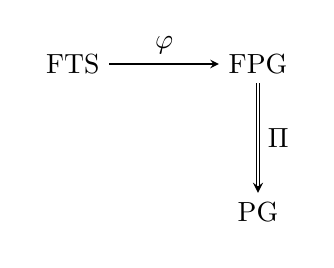
\begin{tikzpicture}
\matrix (m) [matrix of math nodes,row sep=4em,column sep=4em,minimum width=2em]
{
	\text{FTS} & \text{FPG} \\
	\  & \text{PG} \\};
\path[-stealth]
(m-1-1)
edge node [above] {$\varphi$} (m-1-2)

(m-1-2) edge [double] node [right] {$\Pi$} (m-2-2)
;
\end{tikzpicture}\\
Earlier we saw that we could also derive a PG by projecting the FTS to a product and then translation the resulting LTS to a PG, depicted by the following diagram:
\\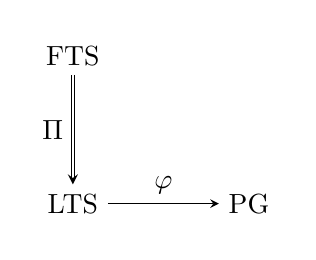
\begin{tikzpicture}
\matrix (m) [matrix of math nodes,row sep=4em,column sep=4em,minimum width=2em]
{
	\text{FTS} \\
	\text{LTS} & \text{PG} \\};
\path[-stealth]
(m-1-1) edge [double] node [left] {$\Pi$} (m-2-1)
(m-2-1.east|-m-2-2) edge node [above] {$\varphi$}
(m-2-2)
;
\end{tikzpicture}\\
We will now show that the resulting parity games are identical.
\begin{theorem}
	\label{the_PGsubPGA} Given:
	\begin{itemize}
		\item FTS $M = (S,Act, trans, s_0, N, P, \gamma)$,
		\item a closed modal mu-calculus formula $\varphi$,
		\item a product $p \in P$
	\end{itemize}
	it holds that the parity games LTS2PG($M_{|p}, \varphi$) and FTS2FPG($M, \varphi$)$_{|p}$  are identical.
	\begin{proof}
		Let $G^F = FTS2FPG(M, \varphi) = (V^F, V_0^F, V_1^F, E^F, \rho^F, N, P, \gamma')$, using definition \ref{def_FTS2FPG}, and $G^F_{|p} = (V^F, V_0^F, V_1^F, {E^F}', \rho^F)$, using definition \ref{def_FPG_proj}. Furthermore we have $M_{|p} = (S, Act, trans', s_0)$ and we let $G =  LTS2PG(M_{|p}, \varphi) = (V, V_0, V_1, E, \rho)$. We depict the different transition systems and games in the following diagram.
		
		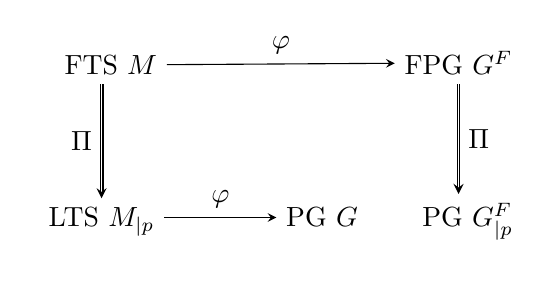
\begin{tikzpicture}
		\matrix (m) [matrix of math nodes,row sep=4em,column sep=1em,minimum width=2em]
		{
			\text{\ \ FTS }M & \  &\ & \text{FPG } G^F  \\
			\text{LTS }M_{|p} & \ & \text{PG } G & \text{\ \ PG }G_{|p}^F \\};
		\path[-stealth]
		(m-1-1) edge [double] node [left] {$\Pi$} (m-2-1)
		edge node [above] {$\varphi$} (m-1-4)
		(m-2-1.east|-m-2-3) edge node [above] {$\varphi$}
		(m-2-3)
		(m-1-4) edge [double] node [right] {$\Pi$} (m-2-4);
		\end{tikzpicture}\\
		We will prove that $G = G_{|p}^F$. We first note that game $G$ is created by 
		\[  (V, V_0, V_1, E, \rho) = LTS2PG((S, Act, trans', s_0),\varphi) \]
		and the vertices, edges and priorities of game $G^F$ are created by 
		\[ (V^F, V_0^F, V_1^F, E^F, \rho^F) = LTS2PG((S,Act, trans, s_0), \varphi)\]
		Using the definition of LTS2PG (\ref{def_LTS2PG}) we find that the vertices and the priorities only depend on the states in $S$ and the formula $\varphi$, since these are identical in the above two statements we immediately get $V = V^F, V_0 = V_0^F, V_1 = V_1^F$ and $\rho = \rho^F$. The vertices and priorities don't change when an FTS is projected, therefore $G_{|p}^F$ has the same vertices and priorities as $G^F$.
		
		Now we are left with showing that $E = {E^F}'$ in order to conclude that that $G = G^F_{|p}$. We will do this by showing $E \subseteq {E^F}'$ and $E \supseteq {E^F}'$.
		
		First let $e \in E$. Note that a vertex in the parity game is represented by a pair of a state and a formula. So we can write $e = ((s,\psi),(s',\psi'))$. To show that $e \in {E^F}'$ we distinguish two cases:
		\begin{itemize}
			\item  If $\psi = \langle a \rangle \psi_1$ or $\psi = [a] \psi_1$ then there exists an $a \in Act$ such that $(s,a,s') \in trans'$. Using definition the FTS projection definition (\ref{def_fts_proj}) we get $(s,a,s') \in trans$ and $p \models \gamma(s,a,s')$. Using the $FTS2FPG$ definition (\ref{def_FTS2FPG}) we find that $\gamma'((s,\psi),(s',\psi')) = \gamma(s,a,s')$ and therefore $p \models \gamma'((s,\psi),(s',\psi'))$. Now using the FPG projection definition (\ref{def_FPG_proj}) we find $((s,\psi),(s',\psi')) \in {E^F}'$.
			\item Otherwise the existence of the edge does not depend on the $trans$ parameter and therefore $((s,\psi),(s',\psi')) \in {E^F}'$ if $(s,\psi) \in V^F$, since $V^F = V$ we have $(s,\psi) \in V^F$.
		\end{itemize}
		We can conclude that $E \subseteq {E^F}'$, next we will show $E \supseteq {E^F}'$. Let $e = ((s,\psi),(s',\psi')) \in {E^F}'$. We distinguish two cases:
		\begin{itemize}
			\item If $\psi = \langle a \rangle \psi_1$ or $\psi = [a] \psi_1$ then there exists an $a \in Act$ such that $(s,a,s') \in trans$. Using the FPG projection definition (\ref{def_FPG_proj}) we get $p \models \gamma'(s,a,s')$. Using the $FTS2FPG$ definition (\ref{def_FTS2FPG}) we get $p \models \gamma(s,a,s')$. Using the projection definition (\ref{def_FTS2FPG}) we get $(s,a,s') \in trans'$ and therefore $((s,\psi),(s',\psi'))\in E$.
			\item Otherwise the existence of the edge does not depend on the $trans$ parameter and therefore $((s,\psi),(s',\psi')) \in E$ if $(s,\psi) \in V$, since $V^F = V$ we have $(s,\psi) \in V$.
		\end{itemize}
	\end{proof}
\end{theorem}

Having proven this we can visualize the relation between the different games and transition systems in the following diagram:
\\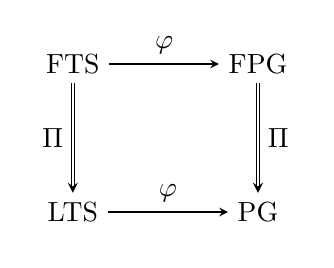
\begin{tikzpicture}
\matrix (m) [matrix of math nodes,row sep=4em,column sep=4em,minimum width=2em]
{
	\text{FTS} & \text{FPG} \\
	\text{LTS} & \text{PG} \\};
\path[-stealth]
(m-1-1) edge [double] node [left] {$\Pi$} (m-2-1)
edge node [above] {$\varphi$} (m-1-2)
(m-2-1.east|-m-2-2) edge node [above] {$\varphi$}
(m-2-2)
(m-1-2) edge [double] node [right] {$\Pi$} (m-2-2)
;
\end{tikzpicture}\\
Finally we prove that solving an FTS, ie. finding winning sets for all products, answers the verification question.
\begin{theorem}
	\label{the_FPG_ver_FTS}
	Given:
	\begin{itemize}
		\item FTS $M = (S, Act, trans, s_0, N, P, \gamma)$,
		\item closed modal mu-calculus formula $\varphi$,
		\item product $p \in P$ and
		\item state $s \in S$
	\end{itemize}
	it holds that $M_{|p}, s \models \varphi$ if and only if $(s, \varphi) \in W_0^p$ in FTS2FPG($M, \varphi$).
	\begin{proof}
		The winning set $W_\alpha^p$ is equal to winning set $W_\alpha$ in $FTS2FPG(M, \varphi)_{|p}$, for any $\alpha \in \{0,1\}$, using the FPG definition (\ref{def_FPG}). Using theorem \ref{the_PGsubPGA} we find that the game $FTS2FPG(M, \varphi)_{|p}$ is equal to the game $LTS2PG(M_{|p}, \varphi)$, obviously their winning sets are also equal. Using the well studied relation between parity games and LTS verification, stated in theorem \ref{the_LTS_PG_REL}, we know that $M_{|p}, s \models \varphi$ if and only if $(s, \varphi) \in W_0$ in game $LTS2PG(M_{|p},\varphi)$. Winning set $W_\alpha^p$ is equal to $W_\alpha$, therefore the theorem holds.
	\end{proof}
\end{theorem}

Revisiting our prior example we can see the theorem in action by noting that $M_{|\emptyset} \models \varphi$ , $M_{|\{f\}} \not\models \varphi$ and $M_{|\{f,g\}} \models \varphi$. This is reflected by the vertex $(s_1, \mu X. [a]X \vee \langle b \rangle \top)$ being present in $W_0^\emptyset$ and $W_0^{\{f,g\}}$ but not in $W_0^{\{f\}}$.

\section{Variability parity games}
Next we will introduce \textit{variability parity games} (VPGs). VPGs are very similar to FPGs, however VPGs use configurations instead of features and products to express variability. This gives a syntactically more pleasant representation that is not solely tailored for FTSs. Furthermore in VPGs deadlocks are removed, by doing so VPG plays can only result in infinite paths and no longer in finite paths.

Later we will show the relation between VPGs and FTS verification, which is similar to the relation between FPGs and FTS verification. First we introduce VPGs.
\begin{definition}
\label{def_VPG}
A variability parity game (VPG) is a tuple $(V,V_0, V_1, E, \Omega, \mathfrak{C}, \theta)$, where:
\begin{itemize}
	\item $V = V_0 \cup V_1$ and $V_0 \cap V_1 = \emptyset$,
	\item $V_0$ is the set of vertices owned by player $0$,
	\item $V_1$ is the set of vertices owned by player $1$, 
	\item $E \subseteq V \times V$ is the edge relation; we assume that $E$ is total, i.e. for all $v\in V$ there is some $w \in V$ such that $(v,w) \in E$,
	\item $\Omega :  V \rightarrow \mathbb{N}$ is a priority assignment,
	\item $\mathfrak{C}$ is a non-empty finite set of configurations,
	\item $\theta : E \rightarrow \mathcal{P}(\mathfrak{C})\ \backslash\ \{0\}$ is the configuration mapping, satisfying for all $v \in V$, $\bigcup\{\theta(v,w)\ |\ (v,w) \in E\} = \mathfrak{C}$.
\end{itemize}
\end{definition}
A VPG is played similarly to a PG, however the game is played for a specific configuration $c \in \mathfrak{C}$. Player $\alpha$ can only move the token from $v \in V_\alpha$ to $w \in V$ if $(v,w) \in E$ and $c \in \theta(v,w)$. Furthermore VPGs don't have deadlocks, therefore every play results in an infinite path.

A game played for configuration $c \in \mathfrak{C}$ results in winning sets $W_0^c$ and $W_1^c$, which are defined similar to the $W_0$ and $W_1$ winning sets for parity games.

Solving a VPG means determining winning sets for every configuration in the VPG.
\begin{definition}
\label{def_VPG_proj} The projection from VPG $G = (V, V_0, V_1, E, \Omega, \mathfrak{C}, \theta)$ to a configuration $c \in \mathfrak{C}$, noted $G_{|c}$, is the parity game $(V, V_0, V_1, E', \Omega)$ where $E' = \{ e\in E\ |\ c \in \theta(e)\}$.
\end{definition}

Playing VPG $G$ for a specific configuration $c \in \mathfrak{C}$ is the same as playing the PG $G_{|c}$. Any path that is valid in $G$ for $c$ is also valid in $G_{|c}$ and vice versa. Therefore the strategies are also interchangeable, furthermore the winning sets $W_\alpha$ for $G_{|c}$ and $W_\alpha^c$ for $G$ are identical. Since parity games are positionally determined so are VPGs. Similarly, since finite parity games are decidable, so are finite VPGs.
\subsection{Creating variability parity games}
We will define a translation from an FPG to a VPG. To do so we use the set of valid products as the set of configurations. Furthermore we make the FPG deadlock free, this is done by creating two losing vertices $l_0$ and $l_1$ such that player $\alpha$ loses when the token is in vertex $l_\alpha$. Any vertex that can't move for a configuration will get an edge that is admissible for that configuration towards one of the losing vertices.
\begin{definition}
	\label{def_FPG2VPG}
	FPG2VPG($G^F$) converts FPG $G^F = (V^F, V_0^F, V_1^F, E^F, \Omega^F, N, P, \gamma)$ to VPG $G = (V, V_0, V_1, E, \Omega, \mathfrak{C}, \theta)$.
	
	We define $\mathfrak{C} = P$. We create vertices $l_0$ and $l_1$ and define $V_0 = V_0^F \cup \{l_0\}$, $V_1 = V_1^F \cup \{l_1\}$ and $V = V_0 \cup V_1$.
	
	We construct $E$ by first making $E = E^F$ and adding edges $(l_0, l_0)$ and $(l_1, l_1)$ to $E$. Simultaneously we construct $\theta$ by first making $\theta(e) = \{p \in \mathfrak{C}\ |\ p \models \gamma(e)\}$ for every $e \in E^F$. Furthermore $\theta(l_0,l_0) = \theta(l_1,l_1) = \mathfrak{C}$.
	
	Next, for every vertex $v \in V_\alpha$ with $\alpha = \{0,1\}$, we have $C = \mathfrak{C} \backslash \bigcup \{\theta(v,w)\ |\ (v,w) \in E\}$. If $C \neq \emptyset$ then we add $(v, l_\alpha)$ to $E$ and make $\theta(v,l_\alpha) = C$.
	Finally we have 
	\[ \Omega(v) = \begin{cases}
	1  & \text{if } v = l_0 \\
	0 & \text{if } v = l_1 \\
	\Omega^F(v) &\text{otherwise}
	\end{cases} \]
\end{definition}
Again considering our previous working example we can translate the FPG shown in figure \ref{fig:exverfpg} to the VPG shown in figure \ref{fig:exvevpg}. Where $c_0$ is product $\emptyset$, $c_1$ is $\{f\}$ and $c_2$ is $\{f,g\}$.
\begin{figure}[h]
	\centering
	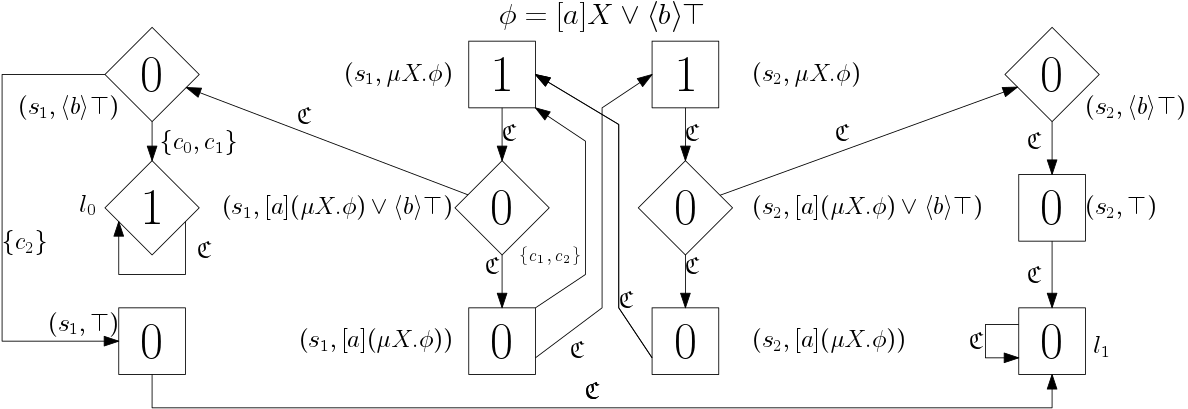
\includegraphics[scale=0.3]{Examples/ExamleVerification/VPG}
	\caption[VPG]{VPG}
	\label{fig:exvevpg}
\end{figure}

\subsection{FTS verification using VPG}
We have shown in theorem \ref{the_FPG_ver_FTS} that we can use an FPG to verify an FTS. Next we will show that a winning set in the FPG $M$ is the subset of the winning set in the VPG $\textit{FPG2VPG}(M)$.
\begin{theorem}
	\label{the_FPG_sub_VPG}
	Given:
	\begin{itemize}
		\item FPG $G^F = (V^F, V_0^F, V_1^F, E^F, \Omega^F, N, P, \gamma)$,
		\item product $p \in P$
	\end{itemize}
	we have for winning sets $Q_\alpha^{p}$ in $G^F$ and $W_\alpha^{p}$ in $\textit{FPG2VPG}(G^F)$ that $Q_\alpha^{p} \subseteq W_\alpha^{p}$ for any $\alpha \in \{0,1\}$.
	\begin{proof}
		Let $G = (V,V_0,V_1, E, \Omega, \mathfrak{C},\theta) = \textit{FPG2VPG}(G^F)$. Consider finite play $\pi$ that is valid in game $G^F$ for product $p$. We have for every $(\pi_i, \pi_{i+1})$ in $\pi$ that $(\pi_i, \pi_{i+1}) \in E^F$ and $p \models \gamma(\pi_i, \pi_{i+1})$. From the $\textit{FPG2VPG}$ definition (\ref{def_FPG2VPG}) it follows that $(\pi_i, \pi_{i+1}) \in E$ and $p \in \theta(\pi_i, \pi_{i+1})$. So we can conclude that path $\pi$ is also valid in game $G$ for configuration $p$. Since the play is finite the winner is determined by the last vertex $v$ in $\pi$, player $\alpha$ wins such that $v \in V_{\overline{\alpha}}$. Furthermore we know, because the play is finite, that there exists no $(v,w) \in E^F$ with $p \models \gamma(v,w)$. From this we can conclude that $(v, l_{\overline{\alpha}}) \in E$ and $p \in \theta(v, l_{\overline{\alpha}})$. Vertex $l_{\overline{\alpha}}$ has one outgoing edge, namely to itself. So finite play $\pi$ will in game $G^F$ results in an infinite play $\pi(l_{\overline{\alpha}})^\omega$. Vertex $l_{\overline{\alpha}}$ has a priority with the same parity as player $\alpha$, so player $\alpha$ wins the infinite play in $G$ for configuration $p$.
		
		Consider infinite play $\pi$ that is valid in game $G^F$ for product $p$. As shown above this play is also valid in game $G$ for configuration $p$. Since the win conditions of both games are the same the play will result in the same winner.
		
		Consider infinite play $\pi$ that is valid in game $G$ for configuration $p$. We distinguish two cases:
		\begin{itemize}
			\item If $l_\alpha$ doesn't occur in $\pi$ then the path is also valid for game $G^F$ with product $p$ and has the same winner.
			\item If $\pi = \pi'(l_\alpha)^\omega$ with no occurrence of $l_\alpha$ in $\pi'$ then the winner is player $\overline{\alpha}$. The path $\pi'$ is valid for game $G^F$ with product $p$. Let vertex $v$ be the last vertex of $\pi'$. Since $(v, l_\alpha) \in E$ and $p \in \theta(v,l_\alpha)$ we know that there is no $(v,w) \in E^F$ with $p \models \gamma(v,w)$ and that vertex $v$ is owned by player $\alpha$. So in game $G^F$ player $\alpha$ can't move at vertex $v$ and therefore loses the game (in which case the winner is also $\overline{\alpha}$).
		\end{itemize}
		
		We have shown that every path (finite or infinite) in game $G^F$ with product $p$ can be played in game $G$ with configuration $p$ and that they have the same winner. Furthermore every infinite path in game $G$ with configuration $p$ can be either played as an infinite path or the first part of the path can be played in $G^F$ with product $p$ and they have the same winner. From this we can conclude that the theorem holds.
	\end{proof}
\end{theorem}
We can conclude the diagram depicting the relation between the different games and transition systems:\\
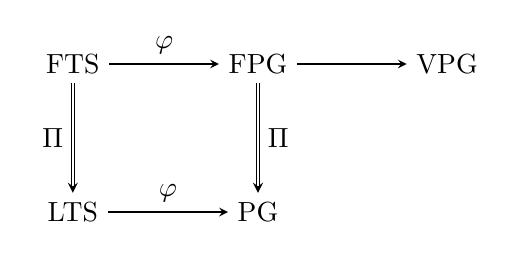
\begin{tikzpicture}
\matrix (m) [matrix of math nodes,row sep=4em,column sep=4em,minimum width=2em]
{
	\text{FTS} & \text{FPG} & \text{VPG} \\
	\text{LTS} & \text{PG} \\};
\path[-stealth]
(m-1-1) edge [double] node [left] {$\Pi$} (m-2-1)
edge node [above] {$\varphi$} (m-1-2)
(m-2-1.east|-m-2-2) edge node [above] {$\varphi$}
(m-2-2)
(m-1-2) edge [double] node [right] {$\Pi$} (m-2-2)
edge (m-1-3);
\end{tikzpicture}\\
Finally we show that solving VPGs, ie. finding the winning sets for all configurations, can be used to verify FTSs.
\begin{theorem}
	\label{the_VPG_ver_FTS}
	Given:
	\begin{itemize}
		\item FTS $M = (S, Act, trans, s_0, N, P, \gamma)$,
		\item closed modal mu-calculus formula $\varphi$,
		\item product $p \in P$ and
		\item state $s \in S$
	\end{itemize}
	it holds that $(M_{|p}, s) \models \varphi$ if and only if $(s, \varphi) \in W_0^{p}$ in $\textit{FPG2VPG}(\textit{FTS2FPG}(M, \varphi))$.
	\begin{proof}
		Let $W_0^{p}$ and $W_1^{p}$ denote the winning sets for game $\textit{FPG2VPG}(\textit{FTS2FPG}(M, \varphi))$. And $Q_0^{p}$ and $Q_1^{p}$ denote the winning sets for game $\textit{FTS2FPG}(M, \varphi)$.
		
		Using theorem \ref{the_FPG_ver_FTS} we find that $(M_{|p}, s) \models \varphi$ if and only if $(s, \varphi) \in Q_0^{p}$. If $(s, \varphi) \in Q_0^{p}$ then we find by using theorem \ref{the_FPG_sub_VPG} that $(s, \varphi) \in W_0^{p}$. If $(s, \varphi) \not\in Q_0^{p}$ then $(s, \varphi) \in Q_1^{p}$ and therefore $(s, \varphi) \in W_1^{p}$ and $(s, \varphi) \not\in W_0^{p}$.
	\end{proof}
\end{theorem}
Using this theorem we can visualize verification of an FTS in figure \ref{fig:ftsverificationusingvpg}.
\begin{figure}[h]
	\centering
	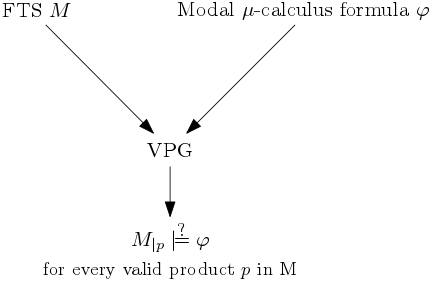
\includegraphics[scale=0.5]{Diagrams/FTSVerificationUsingVPG}
	\caption[FTS verification using VPG]{FTS verification using VPG}
	\label{fig:ftsverificationusingvpg}
\end{figure}

\pagebreak
\part{Solving variability parity games}
\section{Introduction}
For solving VPGs we distinguish two general approaches, the first approach is to simply project the VPG to the different configurations and solve all the resulting parity games independently. We call this approach \textit{product} based. Alternatively we solve the VPG \textit{family} based where a VPG is solved in its entirety and similarities are used to improve performance. 

In this next sections we explore family based algorithms, analyse their running time complexity and present the results of experiments conducted to test the performance of the different family based algorithms compared to the product based approach.

In general we can take some existing algorithm to solve parity games with running time complexity $O(T)$ and use the algorithm to solve a VPG product based. For a VPG with configurations $\mathfrak{C}$ this gives a running time complexity of $O(|\mathfrak{C}|T)$.


\subsection{Preliminaries}
\section{Fixed-point theory} 
A fixed-point of a function is an element in the domain of that function such that the function maps to itself for that element. Fixed-points are used in model verification as well as in some parity game algorithms.

Fixed-point theory goes hand in hand with lattice theory which we introduce first.
\subsection{Lattices}
We introduce definitions for ordering and lattices taken from \cite{birkhoff1940lattice}.
\begin{definition}[\cite{birkhoff1940lattice}]
	A partial order is a binary relation $x \leq y$ on set $S$ where for all $x,y,z \in S$ we have:
	\begin{itemize}
		\item $x \leq x$. (Reflexive)
		\item If $x \leq y$ and $y \leq x$, then $x=y$. (Antisymmetric)
		\item If $x \leq y$ and $y \leq z$, then $x \leq z$. (Transitive)
	\end{itemize}
\end{definition}

\begin{definition}[\cite{birkhoff1940lattice}]
	A partially ordered set is a set $S$ and a partial order $\leq$ for that set, we denote a partially ordered set by $\langle S, \leq \rangle$.
\end{definition}

\begin{definition}[\cite{birkhoff1940lattice}]
	Given partially ordered set $\langle P,\leq \rangle$ and subset $X \subseteq P$. An upper bound to $X$ is an element $a \in P$ such that $x \leq a$ for every $x\in X$. A least upper bound to $X$ is an upper bound $a \in P$ such every other upper bound is larger or equal to $a$.
\end{definition}
The term least upper bound is synonymous with the term supremum, we write $\sup \{ S \}$ to denote the supremum of set $S$.
\begin{definition}[\cite{birkhoff1940lattice}]
	Given partially ordered set $\langle P,\leq \rangle$ and subset $X \subseteq P$. A lower bound to $X$ is an element $a \in P$ such that $a \leq x$ for every $x\in X$. A greatest lower bound to $X$ is a lower bound $a \in P$ such that every other lower bound is smaller or equal to $a$.
\end{definition}
The term greatest lower bound is synonymous with the term infimum, we write $\inf \{ S\}$ to denote the infimum of set $S$.

\begin{definition}[\cite{birkhoff1940lattice}]
	A lattice is a partially ordered set where any two of its elements have a supremum and an infimum.
\end{definition}

\begin{definition}[\cite{birkhoff1940lattice}]
	A complete lattice is a partially ordered set in which every subset has a supremum and an infimum.
\end{definition}

\begin{definition}[\cite{birkhoff1940lattice}]
	Given a lattice $\langle D, \leq \rangle$, function $f : D \rightarrow D$ is monotonic if for all $x \in D$ and $y \in D$ it holds that if $x \leq y$ then $f(x) \leq f(y)$.
\end{definition}
\subsection{Fixed-points}
Fixed-points are formally defined as follows:
\begin{definition}
	Given function $f : D \rightarrow D$ the value $x \in D$ is a fixed-point for $f$ if and only if $f(x) = x$. Furthermore $x$ is the least fixed-point for $f$ if every other fixed-point for $f$ is greater or equal to $x$ and dually $x$ is the greatest fixed-point for $f$ if every other fixed-point $f$ is less or equal to $x$.
\end{definition}
The Knaster-Tarski theorem states that least and greatest fixed-points exist for some domain and function given that a few conditions hold.
The theorem, as written down by Tarski in \cite{tarski1955}, states:
\begin{theorem}[Knaster-Tarski\cite{tarski1955}]
	\label{the_knaster_tarski}
	Let
	\begin{itemize}
		\item $\langle A, \leq \rangle$ be a complete lattice,
		\item $f$ be a monotonic function on $A$ to $A$,
		\item $P$ be the set of all fixpoints of f.
	\end{itemize}
	Then the set $P$ is not empty and the system $\langle P, \leq \rangle$ is a complete lattice; in particular we have 
	\[ \sup P = \sup \{ x\ |\ f(x) \geq x \} \in P \]
	and
	\[ \inf P = \inf \{ x\ |\ f(x) \leq x \} \in P \]
\end{theorem}

\section{Model verification}
It is difficult to develop correct software, one way to improve reliability of software is through model verification; the behaviour of software is specified in a model and formal verification techniques are used to show that the behaviour adheres to certain requirements. In this section we inspect how to model behaviour and how to specify requirements.

Behaviour can be modelled as a \textit{labelled transition system} (LTS). An LTS consists of states in which the system can find itself and transitions between states. Transitions represent the possible state change of the system. Transitions are labelled with actions that indicate what kind of change is happening. Formally we define an LTS as follows.
\begin{definition}[\cite{Groote}]
	\label{def_lts}
	A labelled transition system (LTS) is a tuple $M = (S, Act, trans, s_0)$, where:
	\begin{itemize}
		\item $S$ is a finite set of states,
		\item $Act$ a finite set of actions,
		\item $trans \subseteq S \times Act \times S$ is the transition relation with $(s,a,s') \in trans$ denoted by $s \xrightarrow a s'$,
		\item $s_0 \in S$ is the initial state.
	\end{itemize}
\end{definition}

An LTS is usually depicted as a graph where the vertices represent the states, the edges represent the transitions, edges are labelled with actions and an edge with no origin vertex indicates the initial state. Such a representation is depicted in the example below.
\begin{example}[\cite{FamBasedModelCheckingWithMCRL2}]
	Consider the behaviour of a coffee machine that accepts a coin after which it serves a standard coffee, this can be repeated infinitely often. 
	
	The behaviour can be modelled as an LTS that has two states: in the initial state it is ready to accept a coin and in the second state it is ready to serve a standard coffee. We introduce two actions: \textit{ins}, which represents a coin being inserted, and \textit{std}, which represents a standard coffee being served. We get the following LTS which is also depicted in Figure \ref{fig:coffeemachinebasiceurolts}.
	\[ (\{s_1,s_2\},\{std,ins\},\{(s_1,ins,s_2),(s_2,std,s_1)\},s_1)\]
	\begin{figure}[h]
		\centering
		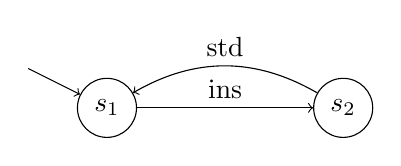
\begin{tikzpicture}[->]
			\tikzstyle{state} = [circle,draw,minimum size=0.75cm]
			
			\node[state] (s1) at (1,0) {$s_1$};
			\node[state] (s2) at (4,0) {$s_2$};
			
			\path (s1) edge node[above]{ins} (s2) ;
			\path (s2) edge[bend right] node[above]{std} (s1) ;
			\path (0,0.5) edge (s1);
		\end{tikzpicture}
		\caption[Coffee machine LTS]{Coffee machine LTS $C$}
		\label{fig:coffeemachinebasiceurolts}
	\end{figure}
\end{example}

LTSs might be non-deterministic, meaning that from a state there might be multiple transitions that can be taken, moreover multiple transitions with the same action can be taken. This is depicted in the example below.

\begin{example}
	We extend the coffee machine example where at some point the coffee machine can be empty and needs a fill before the system is ready to receive a coin again. This LTS is depicted in Figure \ref{fig:coffeemachineundeterministic}. When the \textit{std} transition is taken from state $s_2$ it is non-determined in which states the system ends.
	\begin{figure}[h]
		\centering
		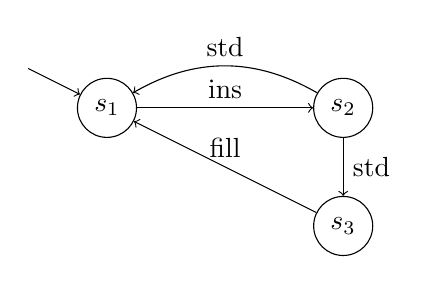
\begin{tikzpicture}[->]
			\tikzstyle{state} = [circle,draw,minimum size=0.75cm]
			
			\node[state] (s1) at (1,1.5) {$s_1$};
			\node[state] (s2) at (4,1.5) {$s_2$};
			\node[state] (s3) at (4,0) {$s_3$};
			
			\path (s1) edge node[above]{ins} (s2) ;
			\path (s2) edge[bend right] node[above]{std} (s1) ;
			\path (s2) edge node [right]{std} (s3);
			\path (s3) edge node [above]{fill} (s1);
			\path (0,2) edge (s1);
		\end{tikzpicture}
		\caption[Coffee machine LTS]{Coffee machine with non-deterministic behaviour}
		\label{fig:coffeemachineundeterministic}
	\end{figure}
\end{example}


A system can be verified by checking if its behaviour adheres to certain requirements. The behaviour can be modelled in an LTS. Requirements can be expressed in a temporal logic; with a temporal logic we can express certain propositions with a time constraint such as \textit{always}, \textit{never} or \textit{eventually}. For example (relating to the coffee machine example) we can express the following constraint: "After a coin is inserted the machine always serves a standard coffee immediately afterwards". The most expressive temporal logic is the modal $\mu$-calculus. A modal $\mu$-calculus formula is expressed over a set of actions and a set of variables.

We define the syntax of the modal $\mu$-calculus below. Note that the syntax is in positive normal form, ie. no negations.
\begin{definition}[\cite{Groote}]
	\label{def_mu_syntax}
	A modal $\mu$-calculus formula over the set of actions $Act$ and a set of variables $\mathcal{X}$ is defined by
	\[ \varphi = \top\ |\ \bot\ |\ X\ |\ \varphi \vee \varphi\ |\ \varphi \wedge \varphi\ |\ \langle a \rangle \varphi\ |\ [a]\varphi\ |\ \mu X.\varphi\ |\ \nu X.\varphi \]
	with $a \in Act$ and $X \in \mathcal{X}$. 
\end{definition}
The modal $\mu$-calculus contains boolean constants $\top$ and $\bot$, propositional operators $\vee$ and $\wedge$, modal operators $\langle \, \rangle$ and $[ \, ]$ and fixpoint operators $\mu$ and $\nu$. 

A variable $X \in \mathcal{X}$ \textit{occurs free} in formula $\phi$ if and only if $X$ occurs in $\phi$ such that $X$ is not a sub-formula of $\mu X.\phi'$ or $\nu X.\phi'$ in $\phi$. A formula is \textit{closed} if and only if there are no variables that occurs free.

A formula can be interpreted in the context of an LTS, such an interpretation results in a set of states in which the formula holds. Given formula $\varphi$ we define the interpretation of $\varphi$ as $\llbracket \varphi \rrbracket ^\eta  \subseteq S$ where $\eta : \mathcal{X}\rightarrow 2^S$ maps a variable to a set of states. We can assign $S' \subseteq S$ to variable $X$ in $\eta$ by writing $\eta[X:=S']$, ie. $(\eta[X:=S'])(X) = S'$.
\begin{definition}
	\label{def_mu_sem} For LTS $(S, Act, trans, s_0)$ we inductively define the interpretation of a modal $\mu$-calculus formula $\varphi$, notation
	$\llbracket \varphi \rrbracket^\eta$, where $\eta : \mathcal{X} \rightarrow \mathcal{P}(S)$ is a variable valuation, as a set of states
	where $\varphi$ is valid, by:
	\begin{align*}
	&\llbracket {\top} \rrbracket^\eta &&= S\\
	&\llbracket {\bot} \rrbracket^\eta &&= \emptyset\\
	&\llbracket \varphi_1 \wedge \varphi_2 \rrbracket^\eta &&= \llbracket \varphi_1 \rrbracket^\eta \cap \llbracket \varphi_2 \rrbracket^\eta \\
	&\llbracket \varphi_1 \vee \varphi_2 \rrbracket^\eta &&= \llbracket \varphi_1 \rrbracket^\eta \cup \llbracket \varphi_2 \rrbracket^\eta\\
	&\llbracket \langle a \rangle \varphi \rrbracket^\eta &&= \{s \in S|\exists_{s' \in S}\ s \xrightarrow {a} s' \wedge s' \in \llbracket \varphi \rrbracket^\eta\}\\
	&\llbracket [ a ] \varphi \rrbracket^\eta &&= \{s \in S|\forall_{s' \in S}\ s \xrightarrow {a} s' \implies s' \in \llbracket \varphi \rrbracket^\eta\}\\
	&\llbracket \mu X. \varphi \rrbracket^\eta &&= \bigcap\{f \subseteq S | f \supseteq \llbracket \varphi \rrbracket^{\eta[X:=f]}\}\\
	&\llbracket \nu X. \varphi \rrbracket^\eta &&= \bigcup\{f \subseteq S | f \subseteq \llbracket \varphi \rrbracket^{\eta[X:=f]}\}\\
	&\llbracket X \rrbracket^\eta &&= \eta(X)
	\end{align*}
\end{definition}
Since there are no negations in the syntax we find that every modal $\mu$-calculus formula is monotone, ie. if we have for $U \subseteq S$ and $U' \subseteq S$ that $U \subseteq U'$ holds then $\llbracket \varphi \rrbracket^{\eta[X:=U]} \subseteq \llbracket \varphi \rrbracket^{\eta[X:=U']}$ holds for any variable $X \in \mathcal{X}$. Using the Knaster-Tarski theorem (Theorem \ref{the_knaster_tarski}) we find that the least and greatest fixed-points always exist.

Given closed formula $\varphi$, LTS $M = (S, Act, trans, s_0)$ and $s \in S$ we say that $M$ satisfies formula $\varphi$ in state $s$, and write $(M,s) \models \varphi$, if and only if $s \in \llbracket \varphi \rrbracket^\eta$. If and only if $M$ satisfies $\varphi$ in the initial state do we say that $M$ satisfies formula $\varphi$ and write $M \models \varphi$. 

\begin{example}[\cite{FamBasedModelCheckingWithMCRL2}]
	Consider the coffee machine example from Figure \ref{fig:coffeemachinebasiceurolts} and formula $\varphi = \nu X. \mu Y([inst]Y \wedge [std]X)$ which states that action \textit{std} must occur infinitely often over all infinite runs. Obviously this holds for the coffee machine, therefore we have $C \models \varphi$.
\end{example}

\section{Parity games}
A \textit{parity game} is a game played by two players: player 0 (also called player \textit{even}) and player 1 (also called player \textit{odd}). We write $\alpha \in \{0,1\}$ to denote an arbitrary player and $\overline{\alpha}$ to denote $\alpha$'s opponent, ie. $\overline{0} = 1$ and $\overline{1} = 0$. A parity game is played on a playing field which is a directed graph where every vertex is owned by either player 0 or player 1. Furthermore every vertex has a natural number, called its \textit{priority}, associated with it.
\begin{definition}[\cite{Bradfield2018}]
	\label{def_PG}
	A parity game is a tuple $(V, V_0, V_1, E, \Omega)$, where:
	\begin{itemize}
		\item $V$ is a finite set of vertices partitioned in sets $V_0$ and $V_1$, containing vertices owned by player 0 and player 1 respectively,
		\item $E \subseteq V \times V$ is the edge relation,
		\item $\Omega :  V \rightarrow \mathbb{N}$ is the priority assignment function.
	\end{itemize}
\end{definition}
Parity games are usually represented as a graph where vertices owned by player 0 are shown as diamonds and vertices owned by player 1 are shown as boxes, furthermore the priorities are depicted as numbers inside the vertices. Such a representation is shown in the example below.

\begin{example}
	Figure \ref{fig:simplepgpg} shows the parity game:
	\[ V_0 = \{v_1,v_4,v_5\},V_1 = \{v_2,v_3\}, V = V_0 \cup V_1\]
	\[ E = \{(v_1,v_2),(v_2,v_1),(v_1,v_3),(v_2,v_4),(v_3,v_4),(v_3,v_5),(v_4,v_4)\}\] 
	\[ \Omega = \{v_1 \mapsto 2, v_2 \mapsto 3, v_3 \mapsto 0, v_4 \mapsto 0, v_5 \mapsto 1 \}\]
	\begin{figure}[h]
		\centering
		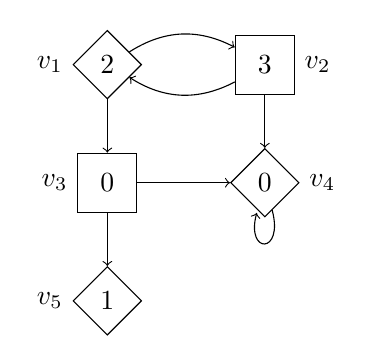
\begin{tikzpicture}[->]
			\tikzstyle{even} = [diamond,draw,minimum size=0.75cm]
			\tikzstyle{odd}  = [rectangle,draw,shape aspect=1,minimum size=0.75cm]
			
			\node[even,label=west:$v_1$] (v1) at (0,3) {2};
			\node[odd, label=east:$v_2$] (v2) at (2,3) {3};
			\node[odd, label=west:$v_3$] (v3) at (0,1.5) {0};
			\node[even,label=east:$v_4$] (v4) at (2,1.5) {0};
			\node[even,label=west:$v_5$] (v5) at (0,0) {1};
			
			\path (v3) edge (v5) ;
			\path (v1) edge [bend left] (v2) ;
			\path (v2) edge [bend left] (v1) ;
			\path (v1) edge (v3) ;
			\path (v3) edge (v4) ;
			\path (v2) edge (v4) ;
			\path (v4) edge [loop below] (v4);
		\end{tikzpicture}
		\caption[Parity game example]{Parity game example}
		\label{fig:simplepgpg}
	\end{figure}
\end{example}

A parity game can be played for a vertex $v \in V$. We start by placing a token on vertex $v$, the player that owns vertex $v$ can choose to move the token along an edge to a vertex $w \in V$ such that $(v,w) \in E$. Again the player that owns vertex $w$ can choose where to move the token next. This is repeated either infinitely often or until a player cannot make a move, ie. the token is on a vertex with no outgoing edges. Playing in this manner gives a sequence of vertices, called a \textit{path}, starting from vertex $v$. For path $\pi$ we write $\pi_i$ to denote $i^\text{th}$ vertex in path $\pi$. Every path is associated with a winner (either player 0 or 1). If a player $\alpha$ cannot move at some point we get a finite path and player $\overline{\alpha}$ wins the path. If we get an infinite path $\pi$ then the winner is determined by the parity of the highest priority that occurs infinitely often in the path. Formally we determine the highest priority occurring infinitely often by the following formula.
\[ \max\{ p \ |\ \forall_j \exists_i j < i \wedge p = \Omega(\pi_i) \}\] 
If the highest priority is odd then player $1$ wins the path, if it is even player $0$ wins the path.

A path is \textit{valid} if and only if for every $i > 0$ such that $\pi_i$ exists we have $(\pi_{i-1},\pi_i) \in E$.


\begin{example}
	Again consider the example in Figure \ref{fig:simplepgpg}. If we play the game for vertex $v_1$ we start by placing a token on $v_1$. Consider the following exemplary paths where $(w_1{\dots}w_m)^\omega$ indicates an infinite repetition of vertices $w_1{\dots}w_m$.
	\begin{itemize}
		\item $\pi = v_1v_3v_5$ is won by player $1$ since player $0$ cannot move at $v_5$.
		\item $\pi = (v_1v_2)^\omega$ is won by player $1$ since the highest priority occurring infinitely often is 3.
		\item $\pi = v_1v_3(v_4)^\omega$ is won by player $0$ since the highest priority occurring infinitely often is $0$.
	\end{itemize}
\end{example}

The moves that the players make are determined by their \textit{strategies}. A strategy $\sigma_\alpha$ determines for a vertex in $V_\alpha$ where the token goes next. We can define a strategy for player $\alpha$ as a partial function $\sigma_\alpha : V^*V_\alpha \rightarrow V$ that maps a series of vertices ending with a vertex owned by player $\alpha$ to the next vertex such that for any $\sigma_\alpha(w_0\dots w_m) = w$ we have $(w_m,w) \in E$. A path $\pi$ \textit{conforms to} strategy $\sigma_\alpha$ if for every $i > 0$ such that $\pi_i$ exists and $\pi_{i-1} \in V_\alpha$ we have $\pi_i = \sigma_\alpha(\pi_0\pi_1\dots\pi_{i-1})$.

A strategy is \textit{winning} for player $\alpha$ from vertex $v$ if and only if $\alpha$ is the winner of every valid path starting in $v$ that conforms to $\sigma_\alpha$. If such a strategy exists for player $\alpha$ from vertex $v$ we say that vertex $v$ is winning for player $\alpha$.

\begin{example}
	In the parity game seen in Figure \ref{fig:simplepgpg} vertex $v_1$ is winning for player 1. Player 1 has a strategy that plays every vertex sequence ending in $v_2$ to $v_1$ and plays every vertex sequence ending in $v_3$ to $v_5$. Regardless of the strategy for player 0 the path will either end up in $v_5$ or will pass $v_2$ infinitely often. In the former case player 1 wins the path because player 0 can not move at $v_5$. In the latter case the highest priority occurring infinitely often is 3.
\end{example}

Parity games are known to be positionally determined \cite{Bradfield2018}, meaning that every vertex in a parity game is winning for one of the two players. Also every player has a \textit{positional strategy} that is winning starting from each of his/her winning vertices. A positional strategy is a strategy that only takes the current vertex into account to determine the next vertex, it does not look at already visited vertices. Therefore we can consider a strategy for player $\alpha$ as a complete functions $\sigma_\alpha : V_\alpha \rightarrow V$. Finally it is decidable for each of the vertices in a parity who the winner is \cite{Bradfield2018}.

A parity game is \textit{solved} if the vertices are partitioned in two sets, namely $W_0$ and $W_1$, such that every vertex in $W_0$ is winning for player 0 and every vertex in $W_1$ is winning for player 1. We call these sets the \textit{winning sets} of a parity game.

Finally parity games are considered \textit{total} if and only if every vertex has at least one outgoing edge. Playing a total parity game always results in an infinite path. We can make a non-total parity game total by adding two sink vertices: $l_0$ and $l_1$. Each sink vertex has only one outgoing edge, namely to itself. Vertex $l_0$ has priority 1 and vertex $l_1$ has priority 0. Clearly if the token ends up in $l_\alpha$ then player $\alpha$ looses the game because with only one outgoing edge we only get a single priority that occurs infinitely often, namely priority $\overline{\alpha}$. For every vertex $v \in V_\alpha$ that does not have an outgoing edge we create an edge from $v$ to $l_\alpha$. In the original game player $\alpha$ lost when the token was in vertex $v$ because he/she could not move any more. In the total game player $\alpha$ can only play to $l_\alpha$ from $v$ where he/she still looses. So using this method vertices in the total game have the same winner as they had in the original game (except for $l_0$ and $l_1$ which did not exist in the original game). In general we try to only work with total games because no distinction is required between finite paths and infinite paths when reasoning about them, however we will encounter some scenario's where non-total games are still considered.

\subsection{Relation between parity games and model checking}
Verifying LTSs against a modal $\mu$-calculus formula can be done by solving a parity game. This is done by translating an LTS in combination with a formula to a parity game, the solution of the parity game provides the information needed to conclude if the model satisfies the formula. This relation is depicted in Figure \ref{fig:ltsverificationusingpg}. 
\begin{figure}[h]
	\centering
	\begin{tikzpicture}[->]
		\tikzstyle{even} = [diamond,draw,minimum size=0.75cm]
		\tikzstyle{odd}  = [rectangle,draw,shape aspect=1,minimum size=0.75cm]
		
		\node (lts) at (0,5)  {LTS $M$};
		\node (form)at (6,5)  {Modal $\mu$-calculus formula $\varphi$};
		\node (PG)  at (3,2.5){PG};
		\node (check)at (3,0){$M \stackrel{?}{\models} \varphi$};
		
		\path (lts) edge (PG);
		\path (form)edge (PG);
		\path (PG)  edge (check);
	\end{tikzpicture}
	\caption[LTS verification using PG]{LTS verification using PG}
	\label{fig:ltsverificationusingpg}
\end{figure}

We consider a method of creating parity games from an LTS and a modal $\mu$-calculus formula such that there is a special vertex $w$ in the parity game that indicates if the LTS satisfies the formula; if and only if $w$ is won by player 0 is the formula satisfied.

First we introduce the notion of unfolding. A fixpoint formula $\mu X . \varphi$ can be unfolded, resulting in formula $\varphi$ where every occurrence of $X$ is replaced by $\mu X . \varphi$, denoted by $\varphi [ X:= \mu X . \varphi]$. Interpreting a fixpoint formula results in the same set as interpreting its unfolding as shown in \cite{Bradfield2018}; i.e. $[\![\mu X . \varphi]\!]^\eta = [\![\varphi[X:=\mu X . \varphi]]\!]^\eta$. The same holds for the fixpoint operator $\nu$.

Next we define the Fischer-Ladner closure for a closed $\mu$-calculus formula 
\cite{STREETT1989249,FISCHER1979194}. The Fischer-Ladner closure of $\varphi$ is the set $\textit{FL}(\varphi)$ of closed formulas containing at least $\varphi$. Furthermore for every formula $\psi$ in $\textit{FL}(\varphi)$ it holds that for every direct subformula $\psi'$ of $\psi$ there is a formula in $\textit{FL}(\varphi)$ that is equivalent to $\psi'$.
\begin{definition}
	\label{def_FLClosure}
	The Fischer-Ladner closure of closed $\mu$-calculus formula $\varphi$ is the smallest set $\textit{FL}(\varphi)$ satisfying the following constraints:
	\begin{itemize}
		\item $\varphi \in \textit{FL}(\varphi)$,
		\item if $\varphi_1 \vee \varphi_2 \in \textit{FL}(\varphi)$ then $\varphi_1 ,\varphi_2 \in \textit{FL}(\varphi)$,
		\item if $\varphi_1 \wedge \varphi_2 \in \textit{FL}(\varphi)$ then $\varphi_1 ,\varphi_2 \in \textit{FL}(\varphi)$,
		\item if $\langle a \rangle \varphi' \in \textit{FL}(\varphi)$ then $\varphi' \in \textit{FL}(\varphi)$,
		\item if $[ a ] \varphi' \in \textit{FL}(\varphi)$ then $\varphi' \in \textit{FL}(\varphi)$,
		\item if $\mu X . \varphi' \in \textit{FL}(\varphi)$ then $\varphi'[X:= \mu X . \varphi'] \in \textit{FL}(\varphi)$ and
		\item if $\nu X . \varphi' \in \textit{FL}(\varphi)$ then $\varphi'[X:= \nu X . \varphi'] \in \textit{FL}(\varphi)$.
		
	\end{itemize}
\end{definition}

We also define the alternation depth of a formula.
\begin{definition}[\cite{Bradfield2018}]
	The dependency order on bound variables of $\varphi$	is the smallest partial order such that $X \leq_\varphi Y$ if $X$ occurs free in $\sigma Y. \psi$ . The alternation depth of a $\mu$-variable X in formula $\varphi $ is the maximal length of a chain $X_1 \leq_\varphi  \dots \leq_\varphi X_n$ where $X = X_1$, variables $X_1, X_3, \dots$ are $\mu$-variables and variables $X_2, X_4, \dots$ are $\nu$-variables. The alternation depth of a $\nu$-variable is defined similarly. The alternation depth of formula $\varphi$, denoted $adepth(\varphi)$, is the maximum of the alternation depths of the variables bound in $\varphi$, or zero if there are no fixpoints.
\end{definition}
\begin{example}
	Consider the formula $\varphi = \nu X. \mu Y. ([ins]Y \wedge [std] X)$ which states that for an LTS with $Act = \{ ins, std\}$ the action \textit{std} must occur infinitely often over all infinite runs. Since $X$ occurs free in $\mu Y. ([ins] Y \wedge [std]X)$ we have $adepth(Y) = 1$ and $adepth(X) = 2$.
\end{example}
As shown in \cite{Bradfield2018} it holds that formula $\mu X. \psi$ has the same alternation depth as its unfolding $\psi[X:=\mu X. \psi]$. Similarly for the greatest fixpoint. 

Next we define the transformation from an LTS and a formula to a parity game.
\begin{definition}[\cite{Bradfield2018}]
	\label{def_LTS2PG}
	LTS2PG($M, \varphi$) converts LTS $M = (S, Act, trans, s_0)$ and closed formula $\varphi$ to a parity game $(V, V_0, V_1, E, \Omega)$.
	
	Vertices in the parity game are presented as pairs of states and sub-formulas. A vertex is created for every state with every formula in the Fischer-Ladner closure of $\varphi$. We define the set of vertices:
	\[ V = S \times \textit{FL}(\varphi) \]
	
	Vertices have the following owners, successors and priorities:\\
	\begin{center}
		\begin{tabular}{l|l|l|l}
			Vertex & Owner & Successor(s) & Priority \\\hline
			$(s,\bot)$ & 0     &       & 0 \\
			$(s,\top)$ & 1     &      & 0 \\
			$(s,\psi_1 \vee \psi_2)$ & 0       & $(s,\psi_1)$ and $(s,\psi_2)$  & 0 \\
			$(s,\psi_1 \wedge \psi_2)$ & 1       & $(s,\psi_1)$ and $(s,\psi_2)$  & 0 \\
			$(s, \langle a \rangle \psi)$ & 0 & $(s',\psi)$ for every $s \xrightarrow{ a} s'$  & 0 \\
			$(s, [ a ] \psi)$ & 1 & $(s',\psi)$ for every $s \xrightarrow{ a} s'$ & 0 \\
			$(s, \mu X. \psi)$ & 1 & $(s, \psi[X:= \mu X. \psi])$ & $2 \lfloor adepth(X) / 2 \rfloor + 1$ \\
			$(s, \nu X. \psi)$ & 1 & $(s, \psi[X:= \nu X. \psi])$ & $2 \lfloor adepth(X) / 2 \rfloor$
		\end{tabular}
	\end{center}

	Since the Fischer-Ladner formula's are closed we never get a vertex $(s,X)$.
\end{definition}
\begin{example}
	Consider LTS $M$ in Figure \ref{fig:exverltsprojempty} and formula $\varphi = \mu X.([a]X \vee \langle b \rangle \top)$ expressing that on any path reached by $a$'s we can eventually do a $b$ action.
	\begin{figure}[h]
		\centering
		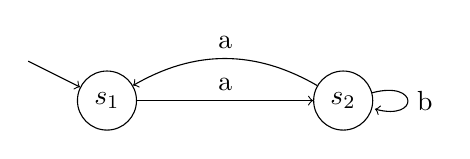
\begin{tikzpicture}[->]
			\tikzstyle{state} = [circle,draw,minimum size=0.75cm]
			
			\node[state] (s1) at (1,1.5) {$s_1$};
			\node[state] (s2) at (4,1.5) {$s_2$};
			
			\path (s1) edge node[above]{a} (s2) ;
			\path (s2) edge[bend right] node[above]{a} (s1) ;
			\path (s2) edge [loop right] node[right]{b} (s2);
			
			\path (0,2) edge (s1);
		\end{tikzpicture}
		\caption[LTS $M$]{LTS $M$}
		\label{fig:exverltsprojempty}
	\end{figure}

	The resulting parity game is depicted in Figure \ref{fig:exverpg}. Let $V$ denote the set of vertices of this parity game. There are two vertices with more than one outgoing edge. From vertex $(s_1, [a](\mu X.\phi) \vee \langle b \rangle \top)$ player 0 does not want to play to $(s_1, \langle b \rangle \top)$ because he/she will not be able to make another move and looses the path. From vertex $(s_2, [a](\mu X.\phi)  \vee \langle b \rangle \top)$ player 0 can play to $(s_2, \langle b \rangle \top)$ to bring the play in $(s_2,\top)$ to win the path. We get the following winning sets:
	\begin{align*}
	W_1 &= \{ (s_1, \langle b \rangle \top )\}\\
	W_0 &= V \backslash W_1
	\end{align*}
	With the strategies $\sigma_0$ for player $0$ and $\sigma_1$ for player $1$ being (vertices with one outgoing edge are omitted):
	\begin{align*}
	\sigma_0 = \{
	&(s_1, [a](\mu X. \phi) \vee \langle b \rangle \top) \mapsto (s_1, [a] (\mu X. \phi)), \\
	&(s_2, [a](\mu X. \phi) \vee \langle b \rangle \top) \mapsto (s_2, \langle b \rangle \top) \} \\
	\sigma_1 = \{&\}
	\end{align*}
	Note that the choice where to go from $(s_2, [a](\mu X.\phi) \vee \langle b \rangle \top)$ does not matter for the winning sets.
	\begin{figure}[h]
		\centering
		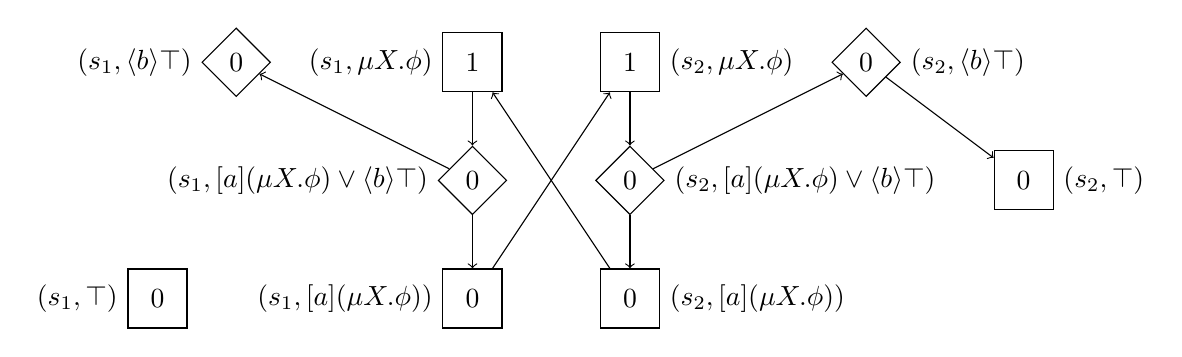
\begin{tikzpicture}[->]
			\tikzstyle{even} = [diamond,draw,minimum size=0.75cm]
			\tikzstyle{odd}  = [rectangle,draw,shape aspect=1,minimum size=0.75cm]
			
			\node[even,label={west:$(s_1,\langle b \rangle\top)$}] (s1<b>T) at (10,10) {0};
			\node[odd,label={west:$(s_1,\top)$}] (s1T) at (9,7) {0};
			
			
			\node[odd,label={west:$(s_1,\mu X.\phi)$}] (s1muxphi) at (13,10) {1};
			\node[even,label={west:$(s_1,[a](\mu X.\phi) \vee \langle b \rangle \top)$}] (s1muxphiunf) at (13,8.5) {0};
			\node[odd,label={west:$(s_1,[a](\mu X .\phi))$}] (s1[a]muxphi) at (13,7) {0};
			
			\node[odd,label={east:$(s_2,\mu X.\phi)$}] (s2muxphi) at (15,10) {1};
			\node[even,label={east:$(s_2,[a](\mu X.\phi) \vee \langle b \rangle \top)$}] (s2muxphiunf) at (15,8.5) {0};
			\node[odd,label={east:$(s_2,[a](\mu X .\phi))$}] (s2[a]muxphi) at (15,7) {0};
			
			
			\node[even,label={east:$(s_2,\langle b \rangle\top)$}] (s2<b>T) at (18,10) {0};
			\node[odd,label={east:$(s_2,\top)$}] (s2T) at (20,8.5) {0};
			
			\path (s1muxphiunf) edge (s1<b>T);
			\path (s1muxphi) edge (s1muxphiunf);
			\path (s1muxphiunf) edge (s1[a]muxphi);
			
			\path (s2muxphiunf) edge (s2<b>T);
			\path (s2muxphi) edge (s2muxphiunf);
			\path (s2muxphiunf) edge (s2[a]muxphi);
			\path (s2<b>T) edge (s2T);
			
			\path(s1[a]muxphi) edge (s2muxphi);
			\path(s2[a]muxphi) edge (s1muxphi);
		\end{tikzpicture}
		
		\caption[Parity game $LTS2PG(M, \varphi)$]{Parity game $LTS2PG(M, \varphi)$ with $\phi = [a] X \vee \langle b \rangle \top$}
		\label{fig:exverpg}
	\end{figure}
\end{example}

Parity games created in this manner relate back to the model verification question; state $s$ in LTS $M$ satisfies $\varphi$ if and only if player $0$ wins vertex $(s, \varphi)$. This is formally stated in the following theorem which is proven in \cite{Bradfield2018}.
\begin{theorem}[\cite{Bradfield2018}]
	\label{the_LTS_PG_REL}Given LTS $M = (S, Act, trans, s_0)$, modal $\mu$-calculus formula $\varphi$ and state $s \in S$ it holds that $(M, s) \models \varphi$ if and only if $(s,\varphi) \in W_0$ for the game $LTS2PG(M, \varphi)$.
\end{theorem}

\subsection{Globally and locally solving parity games}
Parity games can be solved \textit{globally} or \textit{locally}; globally solving a parity game means that for every vertex in the game it is determined who the winner is. Locally solving a parity game means that for a specific vertex in the game it is determined who the winner is. For some applications of parity games, including model checking, there is a specific vertex that needs to be solved to solve the original problem. Locally solving the parity game is sufficient in such cases to solve the original problem.

Most parity game algorithms (including the two considered next) are concerned with globally solving, when talking about solving a parity game we talk about globally solving it unless stated otherwise. 

\subsection{Parity game algorithms}
Various algorithms for solving parity games are known, we introduce two of them. First Zielonka's recursive algorithm which is well studied and generally considered to be one of the best performing parity game algorithms in practice \cite{Oink,SolvingPGInPractice}. We also inspect the fixed-point iteration algorithm which tends to perform well for model-checking problems with a low number of distinct priorities \cite{BDDSolvingPG}.

\subsubsection{Zielonka's recursive algorithm}
First we consider Zielonka's recursive algorithm \cite{ZIELONKA1998135,MCNAUGHTON1993149}, which solves total parity games. Pseudo code is presented in Algorithm \ref{alg_zlnk_org}. Zielonka's recursive algorithm has a worst-case time complexity of $O(e*n^d)$where $e$ is the number of edges, $n$ the number of vertices and $d$ the number of distinct priorities \cite{friedmanPG}.
\begin{algorithm}
	\caption{$\textsc{RecursivePG}(\textit{PG } G = (V,V_0,V_1, E, \Omega))$}
	\label{alg_zlnk_org}
	\begin{algorithmic}[1]
		\If{$V = \emptyset$}
		\State \Return $(\emptyset, \emptyset)$
		\EndIf
		\State $h \gets\max\{ \Omega(v)\ |\ v \in V\}$
		\State $\alpha \gets 0$ if $h$ is even and $1$ otherwise
		\State $U \gets \{v \in V\ |\ \Omega(v) = h\}$
		\State $A \gets \alpha\textit{-Attr}(G, U)$
		\State $(W_0', W_1') \gets \textsc{RecursivePG}(G \backslash A)$
		\If{$W_{\overline{\alpha}}' =\emptyset$}
		\State $W_\alpha \gets A \cup W_\alpha'$
		\State $W_{\overline{\alpha}} \gets \emptyset$
		\Else
		\State $B \gets \overline{\alpha}\textit{-Attr}(G,W_{\overline{\alpha}}')$
		\State $(W_0'', W_1'') \gets \textsc{RecursivePG}(G \backslash B)$
		\State $W_\alpha \gets W_\alpha''$
		\State $W_{\overline{\alpha}} \gets W_{\overline{\alpha}}'' \cup B$
		\EndIf
		\State \Return $(W_0, W_1)$
	\end{algorithmic}
\end{algorithm}

The algorithm solves $G$ by taking the set of vertices with the highest priority and choosing player $\alpha$ such that $\alpha$ has the same parity as the highest priority. Next the algorithm finds set $A$ such that player $\alpha$ can force the play to one of these high priority vertices. Next this set of vertices is removed from $G$ and the resulting subgame $G'$ is solved recursively. 

If $G'$ is entirely won by player $\alpha$ then we distinguish three cases for any path played in $G$. Either the path eventually stays in $G'$, $A$ is infinitely often visited or the path eventually stays in $A$. In the first case player $\alpha$ wins because game $G'$ was entirely won by player $\alpha$. In the second and third case player $\alpha$ can play to the highest priority from $A$. The highest priority, which has parity $\alpha$, is visited infinitely often and player $\alpha$ wins.

If $G'$ is not entirely won by player $\alpha$ we consider winning sets $W'_0$ and $W'_1$ of subgame $G'$. Vertices in set $W'_{\overline{\alpha}}$ are won by player $\overline{\alpha}$ in $G'$ but are also won by player $\overline{\alpha}$ in $G$. The algorithm tries to find all the vertices in $G$ such that player $\overline{\alpha}$ can force the play to a vertex in $W'_{\overline{\alpha}}$ and therefore winning the game. We now have a set of vertices that are definitely won by player $\overline{\alpha}$ in game $G$. In the rest of the game player $\alpha$ can keep the play from $W'_{\overline{\alpha}}$ so the algorithm solves the rest of the game recursively to find the complete winning sets for game $G$.

A complete explanation of the algorithm can be found in \cite{ZIELONKA1998135}, we do introduce definitions for the attractor set and for subgames. 

An attractor set is a set of vertices $A \subseteq V$ calculated for player $\alpha$ given set $U \subseteq V$ where player $\alpha$ has a strategy to force the play starting in any vertex in $A \backslash U$ to a vertex in $U$. Such a set is calculated by adding vertices owned by player $\alpha$ that have an edge to the attractor set and adding vertices owned by player $\overline{\alpha}$ that only have edges to the attractor set.

\begin{definition}[\cite{ZIELONKA1998135}]
	\label{def_attr}Given parity game $G = (V,V_0,V_1,E,\Omega)$ and a non-empty set $U \subseteq V$ we define $\alpha\textit{-Attr}(G,U)$ such that
	\[U_0 = U \]
	For $i \geq 0$:
	\begin{align*}
	U_{i+1} = U_i\cup
	&\{v \in V_\alpha\ |\ \exists v' \in V : v' \in U_i \wedge (v,v') \in E \}\\
	\cup &\{v \in V_{\overline{\alpha}}\ |\ \forall v' \in V :(v,v') \in E \implies v' \in U_i \}
	\end{align*}
	Finally:
	\[\alpha\textit{-Attr}(G,U) = \bigcup_{i \geq 0} U_i \]
\end{definition}

\begin{figure}
	\centering
	\begin{subfigure}{1\textwidth}
		\centering
		\begin{tikzpicture}[->]
			\tikzstyle{even} = [diamond,draw,minimum size=0.75cm]
			\tikzstyle{odd}  = [rectangle,draw,shape aspect=1,minimum size=0.75cm]
			
			\node[even] (v1) at (10,10) {1};
			\node[odd]  (v2) at (11.5,10) {3};
			\node[odd]  (v3) at (13,10) {3};
			\node[even,fill=highlightgraph] (v4) at (14.5,10) {2};
			\node[even] (v5) at (16,10) {2};
			
			\node[even] (v6) at (11.5,8.5) {1};
			\node[odd]  (v7) at (13,8.5) {0};
			\node[even,fill=highlightgraph] (v8) at (14.5,8.5) {0};
			
			\path (v1) edge [bend right] (v2);
			\path (v2) edge [bend right] (v1);
			\path (v2) edge (v3);
			\path (v3) edge (v4);
			\path (v4) edge [bend left] (v5);
			\path (v5) edge [bend left] (v4);
			
			\path (v6) edge (v1);
			\path (v2) edge (v6);
			\path (v6) edge (v3);
			\path (v7) edge (v3);
			\path (v7) edge (v8);
			\path (v3) edge (v8);
			\path (v4) edge [bend left] (v8);
			\path (v8) edge [bend left] (v4);
		\end{tikzpicture}
		\caption{Set $U = U_0$}
	\end{subfigure}\\
	\begin{subfigure}{1\textwidth}
		\centering
		\begin{tikzpicture}[->]
			\tikzstyle{even} = [diamond,draw,minimum size=0.75cm]
			\tikzstyle{odd}  = [rectangle,draw,shape aspect=1,minimum size=0.75cm]
			
			\node[even] (v1) at (10,10) {1};
			\node[odd]  (v2) at (11.5,10) {3};
			\node[odd,fill=highlightgraph]  (v3) at (13,10) {3};
			\node[even,fill=highlightgraph] (v4) at (14.5,10) {2};
			\node[even,fill=highlightgraph] (v5) at (16,10) {2};
			
			\node[even] (v6) at (11.5,8.5) {1};
			\node[odd]  (v7) at (13,8.5) {0};
			\node[even,fill=highlightgraph] (v8) at (14.5,8.5) {0};
			
			\path (v1) edge [bend right] (v2);
			\path (v2) edge [bend right] (v1);
			\path (v2) edge (v3);
			\path (v3) edge (v4);
			\path (v4) edge [bend left] (v5);
			\path (v5) edge [bend left] (v4);
			
			\path (v6) edge (v1);
			\path (v2) edge (v6);
			\path (v6) edge (v3);
			\path (v7) edge (v3);
			\path (v7) edge (v8);
			\path (v3) edge (v8);
			\path (v4) edge [bend left] (v8);
			\path (v8) edge [bend left] (v4);
		\end{tikzpicture}
		\caption{Set $U_1$}
	\end{subfigure}\\
	\begin{subfigure}{1\textwidth}
		\centering
		\begin{tikzpicture}[->]
			\tikzstyle{even} = [diamond,draw,minimum size=0.75cm]
			\tikzstyle{odd}  = [rectangle,draw,shape aspect=1,minimum size=0.75cm]
			
			\node[even] (v1) at (10,10) {1};
			\node[odd]  (v2) at (11.5,10) {3};
			\node[odd,fill=highlightgraph]  (v3) at (13,10) {3};
			\node[even,fill=highlightgraph] (v4) at (14.5,10) {2};
			\node[even,fill=highlightgraph] (v5) at (16,10) {2};
			
			\node[even,fill=highlightgraph] (v6) at (11.5,8.5) {1};
			\node[odd,fill=highlightgraph]  (v7) at (13,8.5) {0};
			\node[even,fill=highlightgraph] (v8) at (14.5,8.5) {0};
			
			\path (v1) edge [bend right] (v2);
			\path (v2) edge [bend right] (v1);
			\path (v2) edge (v3);
			\path (v3) edge (v4);
			\path (v4) edge [bend left] (v5);
			\path (v5) edge [bend left] (v4);
			
			\path (v6) edge (v1);
			\path (v2) edge (v6);
			\path (v6) edge (v3);
			\path (v7) edge (v3);
			\path (v7) edge (v8);
			\path (v3) edge (v8);
			\path (v4) edge [bend left] (v8);
			\path (v8) edge [bend left] (v4);
		\end{tikzpicture}
		\caption{Set $U_2 = 0\textit{-Attr}(G,U)$}
	\end{subfigure}
	\caption{Game $G$ showing the attractor calculation for $0\textit{-Attr}(G,U)$}
	\label{fig:AttrCalcExample}
\end{figure}
\begin{example}
	Figure \ref{fig:AttrCalcExample} shows an example parity game in which an attractor set is calculated for player $0$. For set $U_2$ no more vertices can be attracted so we found the complete attractor set.
\end{example}

The algorithm also creates subgames, where a set of vertices is removed from a parity game to create a new parity game.

\begin{definition}[\cite{ZIELONKA1998135}]
	\label{def_org_subgame}
	Given a parity game $G = (V,V_0,V_1, E,\Omega)$ and $U \subseteq V$ we define the subgame $G \backslash U$ to be the game $(V', V_0', V_1', E', \Omega)$ with:
	\begin{itemize}
		\item $V' = V \backslash U$,
		\item $V_0' = V_0 \cap V'$,
		\item $V_1' = V_1 \cap V'$ and
		\item $E' = E \cap (V' \times V')$.
	\end{itemize}
\end{definition}

Note that a subgame is not necessarily total, however the recursive algorithm always creates subgames that are total (shown in \cite{ZIELONKA1998135}).

\subsubsection{Fixed-point iteration algorithm}
Parity games can be solved by solving an alternating fixed-point formula \cite{WALUKIEWICZ2002311}. Consider PG $G = (V,V_0,V_1, E, \Omega)$ with $d$ distinct priorities. We can apply \textit{priority compression} to make sure every priority in $G$ maps to a value in $\{0,\dots,d-1\}$ or $\{1, \dots, d\}$ \cite{SolvingInPractice,FPITE}. We assume without loss of generality that the priorities map to $\{0,\dots,d-1\}$ and that $d-1$ is even. 

Consider the following formula
\[ S(G) = \nu Z_{d-1}. \mu Z_{d-2}. \dots . \nu Z_0. F_0(G,Z_{d-1},\dots,Z_0) \]
with
\begin{align*}
 F_0(G = (V,V_0,V_1,E,\Omega),Z_{d-1},\dots,Z_0) = &\{ v \in V_0\ |\ \exists_{w\in V}\ (v,w) \in E \wedge w\in Z_{\Omega(w)} \}\\
  \cup &\{ v \in V_1\ |\ \forall_{w\in V}\ (v,w) \in E \implies w\in Z_{\Omega(w)} \}
\end{align*}
where $Z_i \subseteq V$. The formula $\nu X. f(X)$ solves the greatest fixed-point of $X$ in $f$, similarly $\mu X.f(X)$ solves the least fixed-point of $X$ in $f$. As shown in \cite{WALUKIEWICZ2002311} formula $S(G)$ is calculates the set of vertices winning for player 0 in parity game $G$.

To understand the formula we consider sub-formula $\nu Z_0. F_0(Z_{d-1},\dots,Z_0)$. This formula holds for vertices from which player $0$ can either force the play into a node with priority $i > 0$ for which $Z_i$ holds or the player can stay in vertices with priority $0$ indefinitely. The formula $\mu Z_0. F_0(Z_{d-1},\dots,Z_0)$ holds for vertices from which player $0$ can force the play into a node with priority $i > 0$, for which $Z_i$ holds in finitely many steps. By alternating fixed-points the formula allows infinitely many consecutive stays in even vertices and finitely many consecutive stays in odd vertices. For an extensive treatment we refer to \cite{WALUKIEWICZ2002311}.

We further inspect formula $S$. Given game $G$, consider the following sub-formulas:
\[ S^{d-1}(Z_{d-1}) = \mu Z_{d-2}.S^{d-2}(Z_{d-2})\]
\[ S^{d-2}(Z_{d-2}) = \nu Z_{d-3}.S^{d-3}(Z_{d-3})\]
\begin{center}
	\dots
\end{center}
\[ S^{0}(Z_0) = F_0(Z_{d-1},\dots,Z_0)\]
The fixed-point variables are all elements of $2^V$, therefore we have for every sub-formula the following type:
\[ S^i(Z_i) : 2^V \rightarrow 2^V \]
Furthermore, since $V$ is finite, the partially ordered set $\langle 2^V, \subseteq \rangle$ is a complete lattice; for every subset $X \subseteq 2^V$ we have infimum $\bigcap_{x \in X} x$ and supremum $\bigcup_{x \in X} x$. Finally every sub-formula $S^i(Z_i)$ is monotonic, ie. if $S^i(Z_i) \geq S^i(Z_i')$ then $Z_i \geq Z_i'$.

Fixed-point formula's can be solved by \textit{fixed-point iteration}. As shown in \cite{Emerson:1986:MCP:900378} we can calculate $\mu X.f(X)$, where $f$ is monotonic in $X$ and $X \in 2^V$, by iterating $X$:
\[ \mu X.f(X) = \bigcup_{i \geq 0} X^i \]
where $X^i = f(X^{i-1})$ for $i > 0$ and $X^0 \subseteq \mu X.f(X)$. So picking the smallest value possible for $X_0$ will always correctly calculate $\mu X. f(X)$.

Similarly we can calculate fixed-point $\nu X.f(X)$ when $f$ is monotonic in $X$ by iterating $X$:
\[ \nu X.f(X) = \bigcap_{i \geq 0} X^i \]
where $X^i = f(X^{i-1})$ for $i > 0$ and $X^0 \supseteq \nu X.f(X)$. So picking the largest value possible for $X_0$ will always correctly calculate $\nu X. f(X)$.

Since every subformula is monotonic and maps from a value in $2^V$ to another value in $2^V$ we can apply fixed-point iteration to solve the subformula's, we choose initial values $\emptyset$ for least fixed-point variables and $V$ for greatest fixed-point variables.

An algorithm to perform the iteration is presented in \cite{FPITE} and shown in Algorithm \ref{alg_FPITEorg}. This algorithm has a worst-case time complexity of $O(e * n ^d)$ where $e$ is the number of edges, $n$ the number of vertices and $d$ the number of distinct priorities.
\begin{algorithm}
	\caption{Fixed-point iteration}
	\label{alg_FPITEorg}
	\begin{multicols}{2}
		\begin{algorithmic}[1]
			\Function{FPIter}{$G = (V, V_0, V_1, E, \Omega)$}
			\For{$i \gets d-1,\dots,0$}
			\State $\textsc{Init}(i)$
			\EndFor
			\Repeat
			\State $Z_0'\gets Z_0$
			\State $Z_0 \gets \textsc{Diamond}() \cup \textsc{Box}()$
			\State $i \gets 0$
			\While{$Z_i=Z_i' \wedge i < d-1$}
			\State $i \gets i+1$
			\State $Z_i' \gets Z_i$
			\State $Z_i \gets Z_{i-1}$
			\State $\textsc{Init}(i-1)$
			\EndWhile
			\Until{$i = d-1 \wedge Z_{d-1} = Z_{d-1}'$}
			\State \Return $(Z_{d-1},V\backslash Z_{d-1})$
			\EndFunction
		\end{algorithmic}\bigskip\bigskip
		\begin{algorithmic}[1]
			\Function{Init}{$i$}
			\State $Z_i \gets \emptyset$ if $i$ is odd, $V$ otherwise
			\EndFunction
		\end{algorithmic}\bigskip
		\begin{algorithmic}[1]
			\Function{Diamond}{}
			\State \Return $\{ v \in V_0\ |\ \exists_{w\in V} (v,w) \in E \wedge w \in Z_{\Omega(w)}\}$
			\EndFunction
		\end{algorithmic}\bigskip
		\begin{algorithmic}[1]
			\Function{Box}{}
			\State \Return $\{ v \in V_1\ |\ \forall_{w\in V} (v,w) \in E \implies w \in Z_{\Omega(w)}\}$
			\EndFunction
		\end{algorithmic}
	\end{multicols}
\end{algorithm}

\section{Symbolically representing sets}
A set can straightforwardly be represented by a collection containing all the elements that are in the set. We call this an \textit{explicit} representation of a set. We can also represent sets \textit{symbolically} in which case the set of elements is represented by some sort of formula. A typical way to represent a set symbolically is through a boolean formula encoded in a \textit{binary decision diagram} \cite{BDD_book,Handbook_BDD_Chapter}. 

\begin{example}
	\label{ex_boolform}
	The set $S = \{ 2,4,6,7 \}$ can be expressed by boolean formula:
	\[ F(x_2,x_1,x_0) = (\neg x_2 \wedge x_1 \wedge \neg x_0) \vee (x_2 \wedge (x_1 \vee \neg x_0)) \]
	where $x_0,x_1$ and $x_2$ are boolean variables. The formula gives the following truth table:\\
	\begin{center}
		\begin{tabular}{|c|c|}
			\hline 
			$\mathbf{x_2x_1x_0}$ & $\mathbf{F(x_2,x_1,x_0)}$ \\ 
			\hline 
			000 & 0 \\ 
			\hline 
			001 & 0 \\ 
			\hline 
			010 & 1 \\ 
			\hline 
			011 & 0 \\ 
			\hline 
			100 & 1 \\ 
			\hline 
			101 & 0 \\ 
			\hline 
			110 & 1 \\ 
			\hline 
			111 & 1 \\ 
			\hline
		\end{tabular} 
	\end{center}
	The function $F$ defines set $S'$ in the following way: $S' = \{x_2x_1x_0\ |\ F(x_2,x_1,x_0) = 1 \}$. As we can see set $S'$ contains the same numbers as $S$ but represented binary.
\end{example}
We can perform set operations on sets represented as boolean functions by performing logical operations on the functions. For example, given boolean formula's $f$ and $g$ representing sets $V$ and $W$ the formula $f \wedge g$ represents set $V \cap W$.

Given a set $S$ with arbitrary elements we can represent subsets $S' \subseteq S$ as boolean formula's by assigning a number to every element in $S$ and creating a boolean formula that maps boolean variables to true if and only if they represent a number such that the element associated with this number in $S$ is also in $S'$.

\subsection{Binary decision diagrams}
\label{sec_prelim_bdd}
A boolean function can efficiently be represented as a binary decision diagram (BDD), for a comprehensive treatment of BDDs we refer to \cite{BDD_book,Handbook_BDD_Chapter}.

BDDs represent boolean formula's as a directed graph where every vertex represents a boolean variable and has two outgoing edges labelled 0 and 1. Furthermore the graph contains special vertices $0$ and $1$ that have no outgoing edges. We decide if a boolean variable assignment satisfies the formula by starting in the initial vertex of the graph and following a path until we get to either vertex 0 or 1. Since every vertex represents a boolean formula we can create a path from the initial vertex by choosing edge 0 at a vertex if the boolean variable represented by that vertex is false in the variable assignment and choosing edge 1 if is true. Eventually we end up in either vertex 0 or 1. In the former case the boolean variable assignment does not satisfy the formula, in the latter it does.

\begin{example}
	Consider the boolean formula in Example \ref{ex_boolform}. This formula can be represented as the BDD shown in Figure \ref{fig:ex_simplebdd}. The vertices representing boolean variables are shown as circles and the boolean variables they represent are indicated inside them. The special vertices are represented as squares and the initial vertex is represented by an edge with that has no origin vertex.
\begin{figure}[h]
	\centering
	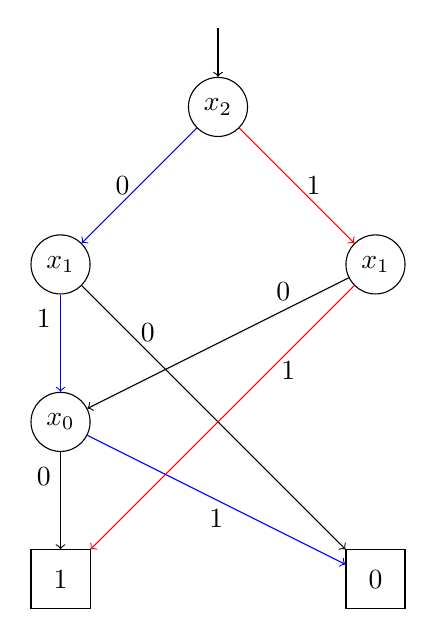
\begin{tikzpicture}[->]
		\tikzstyle{state} = [circle,draw,minimum size=0.75cm]
		\tikzstyle{final}  = [rectangle,draw,shape aspect=1,minimum size=0.75cm]
		
		\node[state] (x2) at (20,20) {$x_2$};
		\node[state] (x10) at (18,18) {$x_1$};
		\node[state] (x11) at (22,18) {$x_1$};
		\node[state] (x0) at (18,16) {$x_0$};
		\node[final] (f1) at (18,14) {$1$};
		\node[final] (f0) at (22,14) {$0$};
		
		\path (20,21) edge (x2);
		\path (x2) edge[blue] node[black,left] {0} (x10);
		\path (x2) edge[red] node[black,right] {1} (x11);
		
		\path (x10) edge[blue] node[black,left,near start] {1} (x0);
		\path (x10) edge[black] node[black,above,near start] {0} (f0);
		
		\path (x11) edge[black] node[black,above,near start] {0} (x0);
		\path (x11) edge[red] node[black,below,near start] {1} (f1);
		
		\path (x0) edge[black] node[black,left,near start] {0} (f1);
		\path (x0) edge[blue] node[black,below] {1} (f0);
	\end{tikzpicture}
	\caption{BDD highlighting boolean variable assignment $x_2x_1x_0 = 011$ in blue and $x_2x_1 = 11$ in red}
	\label{fig:ex_simplebdd}
\end{figure}
	
	The path created from variable assignment $x_2x_1x_0 = 011$ is highlighted in blue in the diagram and shows that this assignment is indeed not satisfied by the boolean formula. The red path shows the variable assignments $110$ and $111$. Determining the path and the outcome for every variable assignment results in the same truth table as seen in Example \ref{ex_boolform}.
\end{example}

Given $n$ boolean variables and two boolean functions encoded as BDDs we can perform binary operations $\vee,\wedge$ on the BDDs in $O(N_a * N_b)$, where $N_a$ and $N_b$ are the number of nodes in the decision diagrams of the two functions. A decision diagram is a tree with $n$ levels, so $N_a = O(2^n)$ and $N_b = O(2^n)$. Therefore with $n$ boolean variables we can perform binary operations $\vee$ and $\wedge$ on them in $O(2^{2n})=O(m^2)$ where $m = 2^n$ is the maximum set size that can be represented by $n$ variables \cite{BDD_running_time,Handbook_BDD_Chapter}. Since the running time specifically depends on the size of the decision diagrams, in general if the boolean functions are simple then the size of the decision diagram is also small and operations can be performed quickly.

\section{Preliminary concepts}
\section{Fixed-point theory} 
A fixed-point of a function is an element in the domain of that function such that the function maps to itself for that element. Fixed-points are used in model verification as well as in some parity game algorithms.

Fixed-point theory goes hand in hand with lattice theory which we introduce first.
\subsection{Lattices}
We introduce definitions for ordering and lattices taken from \cite{birkhoff1940lattice}.
\begin{definition}[\cite{birkhoff1940lattice}]
	A partial order is a binary relation $x \leq y$ on set $S$ where for all $x,y,z \in S$ we have:
	\begin{itemize}
		\item $x \leq x$. (Reflexive)
		\item If $x \leq y$ and $y \leq x$, then $x=y$. (Antisymmetric)
		\item If $x \leq y$ and $y \leq z$, then $x \leq z$. (Transitive)
	\end{itemize}
\end{definition}

\begin{definition}[\cite{birkhoff1940lattice}]
	A partially ordered set is a set $S$ and a partial order $\leq$ for that set, we denote a partially ordered set by $\langle S, \leq \rangle$.
\end{definition}

\begin{definition}[\cite{birkhoff1940lattice}]
	Given partially ordered set $\langle P,\leq \rangle$ and subset $X \subseteq P$. An upper bound to $X$ is an element $a \in P$ such that $x \leq a$ for every $x\in X$. A least upper bound to $X$ is an upper bound $a \in P$ such every other upper bound is larger or equal to $a$.
\end{definition}
The term least upper bound is synonymous with the term supremum, we write $\sup \{ S \}$ to denote the supremum of set $S$.
\begin{definition}[\cite{birkhoff1940lattice}]
	Given partially ordered set $\langle P,\leq \rangle$ and subset $X \subseteq P$. A lower bound to $X$ is an element $a \in P$ such that $a \leq x$ for every $x\in X$. A greatest lower bound to $X$ is a lower bound $a \in P$ such that every other lower bound is smaller or equal to $a$.
\end{definition}
The term greatest lower bound is synonymous with the term infimum, we write $\inf \{ S\}$ to denote the infimum of set $S$.

\begin{definition}[\cite{birkhoff1940lattice}]
	A lattice is a partially ordered set where any two of its elements have a supremum and an infimum.
\end{definition}

\begin{definition}[\cite{birkhoff1940lattice}]
	A complete lattice is a partially ordered set in which every subset has a supremum and an infimum.
\end{definition}

\begin{definition}[\cite{birkhoff1940lattice}]
	Given a lattice $\langle D, \leq \rangle$, function $f : D \rightarrow D$ is monotonic if for all $x \in D$ and $y \in D$ it holds that if $x \leq y$ then $f(x) \leq f(y)$.
\end{definition}
\subsection{Fixed-points}
Fixed-points are formally defined as follows:
\begin{definition}
	Given function $f : D \rightarrow D$ the value $x \in D$ is a fixed-point for $f$ if and only if $f(x) = x$. Furthermore $x$ is the least fixed-point for $f$ if every other fixed-point for $f$ is greater or equal to $x$ and dually $x$ is the greatest fixed-point for $f$ if every other fixed-point $f$ is less or equal to $x$.
\end{definition}
The Knaster-Tarski theorem states that least and greatest fixed-points exist for some domain and function given that a few conditions hold.
The theorem, as written down by Tarski in \cite{tarski1955}, states:
\begin{theorem}[Knaster-Tarski\cite{tarski1955}]
	\label{the_knaster_tarski}
	Let
	\begin{itemize}
		\item $\langle A, \leq \rangle$ be a complete lattice,
		\item $f$ be a monotonic function on $A$ to $A$,
		\item $P$ be the set of all fixpoints of f.
	\end{itemize}
	Then the set $P$ is not empty and the system $\langle P, \leq \rangle$ is a complete lattice; in particular we have 
	\[ \sup P = \sup \{ x\ |\ f(x) \geq x \} \in P \]
	and
	\[ \inf P = \inf \{ x\ |\ f(x) \leq x \} \in P \]
\end{theorem}

\section{Model verification}
It is difficult to develop correct software, one way to improve reliability of software is through model verification; the behaviour of software is specified in a model and formal verification techniques are used to show that the behaviour adheres to certain requirements. In this section we inspect how to model behaviour and how to specify requirements.

Behaviour can be modelled as a \textit{labelled transition system} (LTS). An LTS consists of states in which the system can find itself and transitions between states. Transitions represent the possible state change of the system. Transitions are labelled with actions that indicate what kind of change is happening. Formally we define an LTS as follows.
\begin{definition}[\cite{Groote}]
	\label{def_lts}
	A labelled transition system (LTS) is a tuple $M = (S, Act, trans, s_0)$, where:
	\begin{itemize}
		\item $S$ is a finite set of states,
		\item $Act$ a finite set of actions,
		\item $trans \subseteq S \times Act \times S$ is the transition relation with $(s,a,s') \in trans$ denoted by $s \xrightarrow a s'$,
		\item $s_0 \in S$ is the initial state.
	\end{itemize}
\end{definition}

An LTS is usually depicted as a graph where the vertices represent the states, the edges represent the transitions, edges are labelled with actions and an edge with no origin vertex indicates the initial state. Such a representation is depicted in the example below.
\begin{example}[\cite{FamBasedModelCheckingWithMCRL2}]
	Consider the behaviour of a coffee machine that accepts a coin after which it serves a standard coffee, this can be repeated infinitely often. 
	
	The behaviour can be modelled as an LTS that has two states: in the initial state it is ready to accept a coin and in the second state it is ready to serve a standard coffee. We introduce two actions: \textit{ins}, which represents a coin being inserted, and \textit{std}, which represents a standard coffee being served. We get the following LTS which is also depicted in Figure \ref{fig:coffeemachinebasiceurolts}.
	\[ (\{s_1,s_2\},\{std,ins\},\{(s_1,ins,s_2),(s_2,std,s_1)\},s_1)\]
	\begin{figure}[h]
		\centering
		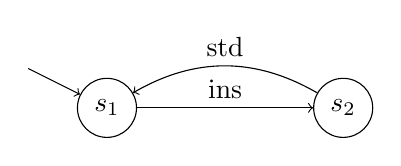
\begin{tikzpicture}[->]
			\tikzstyle{state} = [circle,draw,minimum size=0.75cm]
			
			\node[state] (s1) at (1,0) {$s_1$};
			\node[state] (s2) at (4,0) {$s_2$};
			
			\path (s1) edge node[above]{ins} (s2) ;
			\path (s2) edge[bend right] node[above]{std} (s1) ;
			\path (0,0.5) edge (s1);
		\end{tikzpicture}
		\caption[Coffee machine LTS]{Coffee machine LTS $C$}
		\label{fig:coffeemachinebasiceurolts}
	\end{figure}
\end{example}

LTSs might be non-deterministic, meaning that from a state there might be multiple transitions that can be taken, moreover multiple transitions with the same action can be taken. This is depicted in the example below.

\begin{example}
	We extend the coffee machine example where at some point the coffee machine can be empty and needs a fill before the system is ready to receive a coin again. This LTS is depicted in Figure \ref{fig:coffeemachineundeterministic}. When the \textit{std} transition is taken from state $s_2$ it is non-determined in which states the system ends.
	\begin{figure}[h]
		\centering
		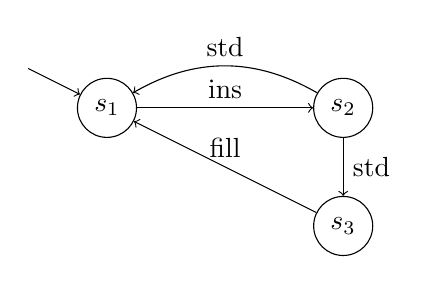
\begin{tikzpicture}[->]
			\tikzstyle{state} = [circle,draw,minimum size=0.75cm]
			
			\node[state] (s1) at (1,1.5) {$s_1$};
			\node[state] (s2) at (4,1.5) {$s_2$};
			\node[state] (s3) at (4,0) {$s_3$};
			
			\path (s1) edge node[above]{ins} (s2) ;
			\path (s2) edge[bend right] node[above]{std} (s1) ;
			\path (s2) edge node [right]{std} (s3);
			\path (s3) edge node [above]{fill} (s1);
			\path (0,2) edge (s1);
		\end{tikzpicture}
		\caption[Coffee machine LTS]{Coffee machine with non-deterministic behaviour}
		\label{fig:coffeemachineundeterministic}
	\end{figure}
\end{example}


A system can be verified by checking if its behaviour adheres to certain requirements. The behaviour can be modelled in an LTS. Requirements can be expressed in a temporal logic; with a temporal logic we can express certain propositions with a time constraint such as \textit{always}, \textit{never} or \textit{eventually}. For example (relating to the coffee machine example) we can express the following constraint: "After a coin is inserted the machine always serves a standard coffee immediately afterwards". The most expressive temporal logic is the modal $\mu$-calculus. A modal $\mu$-calculus formula is expressed over a set of actions and a set of variables.

We define the syntax of the modal $\mu$-calculus below. Note that the syntax is in positive normal form, ie. no negations.
\begin{definition}[\cite{Groote}]
	\label{def_mu_syntax}
	A modal $\mu$-calculus formula over the set of actions $Act$ and a set of variables $\mathcal{X}$ is defined by
	\[ \varphi = \top\ |\ \bot\ |\ X\ |\ \varphi \vee \varphi\ |\ \varphi \wedge \varphi\ |\ \langle a \rangle \varphi\ |\ [a]\varphi\ |\ \mu X.\varphi\ |\ \nu X.\varphi \]
	with $a \in Act$ and $X \in \mathcal{X}$. 
\end{definition}
The modal $\mu$-calculus contains boolean constants $\top$ and $\bot$, propositional operators $\vee$ and $\wedge$, modal operators $\langle \, \rangle$ and $[ \, ]$ and fixpoint operators $\mu$ and $\nu$. 

A variable $X \in \mathcal{X}$ \textit{occurs free} in formula $\phi$ if and only if $X$ occurs in $\phi$ such that $X$ is not a sub-formula of $\mu X.\phi'$ or $\nu X.\phi'$ in $\phi$. A formula is \textit{closed} if and only if there are no variables that occurs free.

A formula can be interpreted in the context of an LTS, such an interpretation results in a set of states in which the formula holds. Given formula $\varphi$ we define the interpretation of $\varphi$ as $\llbracket \varphi \rrbracket ^\eta  \subseteq S$ where $\eta : \mathcal{X}\rightarrow 2^S$ maps a variable to a set of states. We can assign $S' \subseteq S$ to variable $X$ in $\eta$ by writing $\eta[X:=S']$, ie. $(\eta[X:=S'])(X) = S'$.
\begin{definition}
	\label{def_mu_sem} For LTS $(S, Act, trans, s_0)$ we inductively define the interpretation of a modal $\mu$-calculus formula $\varphi$, notation
	$\llbracket \varphi \rrbracket^\eta$, where $\eta : \mathcal{X} \rightarrow \mathcal{P}(S)$ is a variable valuation, as a set of states
	where $\varphi$ is valid, by:
	\begin{align*}
	&\llbracket {\top} \rrbracket^\eta &&= S\\
	&\llbracket {\bot} \rrbracket^\eta &&= \emptyset\\
	&\llbracket \varphi_1 \wedge \varphi_2 \rrbracket^\eta &&= \llbracket \varphi_1 \rrbracket^\eta \cap \llbracket \varphi_2 \rrbracket^\eta \\
	&\llbracket \varphi_1 \vee \varphi_2 \rrbracket^\eta &&= \llbracket \varphi_1 \rrbracket^\eta \cup \llbracket \varphi_2 \rrbracket^\eta\\
	&\llbracket \langle a \rangle \varphi \rrbracket^\eta &&= \{s \in S|\exists_{s' \in S}\ s \xrightarrow {a} s' \wedge s' \in \llbracket \varphi \rrbracket^\eta\}\\
	&\llbracket [ a ] \varphi \rrbracket^\eta &&= \{s \in S|\forall_{s' \in S}\ s \xrightarrow {a} s' \implies s' \in \llbracket \varphi \rrbracket^\eta\}\\
	&\llbracket \mu X. \varphi \rrbracket^\eta &&= \bigcap\{f \subseteq S | f \supseteq \llbracket \varphi \rrbracket^{\eta[X:=f]}\}\\
	&\llbracket \nu X. \varphi \rrbracket^\eta &&= \bigcup\{f \subseteq S | f \subseteq \llbracket \varphi \rrbracket^{\eta[X:=f]}\}\\
	&\llbracket X \rrbracket^\eta &&= \eta(X)
	\end{align*}
\end{definition}
Since there are no negations in the syntax we find that every modal $\mu$-calculus formula is monotone, ie. if we have for $U \subseteq S$ and $U' \subseteq S$ that $U \subseteq U'$ holds then $\llbracket \varphi \rrbracket^{\eta[X:=U]} \subseteq \llbracket \varphi \rrbracket^{\eta[X:=U']}$ holds for any variable $X \in \mathcal{X}$. Using the Knaster-Tarski theorem (Theorem \ref{the_knaster_tarski}) we find that the least and greatest fixed-points always exist.

Given closed formula $\varphi$, LTS $M = (S, Act, trans, s_0)$ and $s \in S$ we say that $M$ satisfies formula $\varphi$ in state $s$, and write $(M,s) \models \varphi$, if and only if $s \in \llbracket \varphi \rrbracket^\eta$. If and only if $M$ satisfies $\varphi$ in the initial state do we say that $M$ satisfies formula $\varphi$ and write $M \models \varphi$. 

\begin{example}[\cite{FamBasedModelCheckingWithMCRL2}]
	Consider the coffee machine example from Figure \ref{fig:coffeemachinebasiceurolts} and formula $\varphi = \nu X. \mu Y([inst]Y \wedge [std]X)$ which states that action \textit{std} must occur infinitely often over all infinite runs. Obviously this holds for the coffee machine, therefore we have $C \models \varphi$.
\end{example}

\section{Parity games}
A \textit{parity game} is a game played by two players: player 0 (also called player \textit{even}) and player 1 (also called player \textit{odd}). We write $\alpha \in \{0,1\}$ to denote an arbitrary player and $\overline{\alpha}$ to denote $\alpha$'s opponent, ie. $\overline{0} = 1$ and $\overline{1} = 0$. A parity game is played on a playing field which is a directed graph where every vertex is owned by either player 0 or player 1. Furthermore every vertex has a natural number, called its \textit{priority}, associated with it.
\begin{definition}[\cite{Bradfield2018}]
	\label{def_PG}
	A parity game is a tuple $(V, V_0, V_1, E, \Omega)$, where:
	\begin{itemize}
		\item $V$ is a finite set of vertices partitioned in sets $V_0$ and $V_1$, containing vertices owned by player 0 and player 1 respectively,
		\item $E \subseteq V \times V$ is the edge relation,
		\item $\Omega :  V \rightarrow \mathbb{N}$ is the priority assignment function.
	\end{itemize}
\end{definition}
Parity games are usually represented as a graph where vertices owned by player 0 are shown as diamonds and vertices owned by player 1 are shown as boxes, furthermore the priorities are depicted as numbers inside the vertices. Such a representation is shown in the example below.

\begin{example}
	Figure \ref{fig:simplepgpg} shows the parity game:
	\[ V_0 = \{v_1,v_4,v_5\},V_1 = \{v_2,v_3\}, V = V_0 \cup V_1\]
	\[ E = \{(v_1,v_2),(v_2,v_1),(v_1,v_3),(v_2,v_4),(v_3,v_4),(v_3,v_5),(v_4,v_4)\}\] 
	\[ \Omega = \{v_1 \mapsto 2, v_2 \mapsto 3, v_3 \mapsto 0, v_4 \mapsto 0, v_5 \mapsto 1 \}\]
	\begin{figure}[h]
		\centering
		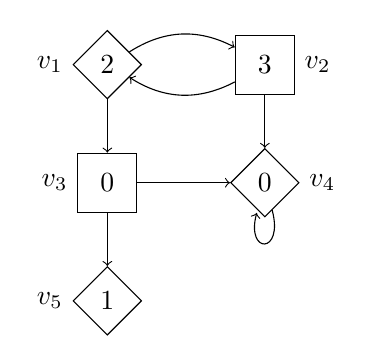
\begin{tikzpicture}[->]
			\tikzstyle{even} = [diamond,draw,minimum size=0.75cm]
			\tikzstyle{odd}  = [rectangle,draw,shape aspect=1,minimum size=0.75cm]
			
			\node[even,label=west:$v_1$] (v1) at (0,3) {2};
			\node[odd, label=east:$v_2$] (v2) at (2,3) {3};
			\node[odd, label=west:$v_3$] (v3) at (0,1.5) {0};
			\node[even,label=east:$v_4$] (v4) at (2,1.5) {0};
			\node[even,label=west:$v_5$] (v5) at (0,0) {1};
			
			\path (v3) edge (v5) ;
			\path (v1) edge [bend left] (v2) ;
			\path (v2) edge [bend left] (v1) ;
			\path (v1) edge (v3) ;
			\path (v3) edge (v4) ;
			\path (v2) edge (v4) ;
			\path (v4) edge [loop below] (v4);
		\end{tikzpicture}
		\caption[Parity game example]{Parity game example}
		\label{fig:simplepgpg}
	\end{figure}
\end{example}

A parity game can be played for a vertex $v \in V$. We start by placing a token on vertex $v$, the player that owns vertex $v$ can choose to move the token along an edge to a vertex $w \in V$ such that $(v,w) \in E$. Again the player that owns vertex $w$ can choose where to move the token next. This is repeated either infinitely often or until a player cannot make a move, ie. the token is on a vertex with no outgoing edges. Playing in this manner gives a sequence of vertices, called a \textit{path}, starting from vertex $v$. For path $\pi$ we write $\pi_i$ to denote $i^\text{th}$ vertex in path $\pi$. Every path is associated with a winner (either player 0 or 1). If a player $\alpha$ cannot move at some point we get a finite path and player $\overline{\alpha}$ wins the path. If we get an infinite path $\pi$ then the winner is determined by the parity of the highest priority that occurs infinitely often in the path. Formally we determine the highest priority occurring infinitely often by the following formula.
\[ \max\{ p \ |\ \forall_j \exists_i j < i \wedge p = \Omega(\pi_i) \}\] 
If the highest priority is odd then player $1$ wins the path, if it is even player $0$ wins the path.

A path is \textit{valid} if and only if for every $i > 0$ such that $\pi_i$ exists we have $(\pi_{i-1},\pi_i) \in E$.


\begin{example}
	Again consider the example in Figure \ref{fig:simplepgpg}. If we play the game for vertex $v_1$ we start by placing a token on $v_1$. Consider the following exemplary paths where $(w_1{\dots}w_m)^\omega$ indicates an infinite repetition of vertices $w_1{\dots}w_m$.
	\begin{itemize}
		\item $\pi = v_1v_3v_5$ is won by player $1$ since player $0$ cannot move at $v_5$.
		\item $\pi = (v_1v_2)^\omega$ is won by player $1$ since the highest priority occurring infinitely often is 3.
		\item $\pi = v_1v_3(v_4)^\omega$ is won by player $0$ since the highest priority occurring infinitely often is $0$.
	\end{itemize}
\end{example}

The moves that the players make are determined by their \textit{strategies}. A strategy $\sigma_\alpha$ determines for a vertex in $V_\alpha$ where the token goes next. We can define a strategy for player $\alpha$ as a partial function $\sigma_\alpha : V^*V_\alpha \rightarrow V$ that maps a series of vertices ending with a vertex owned by player $\alpha$ to the next vertex such that for any $\sigma_\alpha(w_0\dots w_m) = w$ we have $(w_m,w) \in E$. A path $\pi$ \textit{conforms to} strategy $\sigma_\alpha$ if for every $i > 0$ such that $\pi_i$ exists and $\pi_{i-1} \in V_\alpha$ we have $\pi_i = \sigma_\alpha(\pi_0\pi_1\dots\pi_{i-1})$.

A strategy is \textit{winning} for player $\alpha$ from vertex $v$ if and only if $\alpha$ is the winner of every valid path starting in $v$ that conforms to $\sigma_\alpha$. If such a strategy exists for player $\alpha$ from vertex $v$ we say that vertex $v$ is winning for player $\alpha$.

\begin{example}
	In the parity game seen in Figure \ref{fig:simplepgpg} vertex $v_1$ is winning for player 1. Player 1 has a strategy that plays every vertex sequence ending in $v_2$ to $v_1$ and plays every vertex sequence ending in $v_3$ to $v_5$. Regardless of the strategy for player 0 the path will either end up in $v_5$ or will pass $v_2$ infinitely often. In the former case player 1 wins the path because player 0 can not move at $v_5$. In the latter case the highest priority occurring infinitely often is 3.
\end{example}

Parity games are known to be positionally determined \cite{Bradfield2018}, meaning that every vertex in a parity game is winning for one of the two players. Also every player has a \textit{positional strategy} that is winning starting from each of his/her winning vertices. A positional strategy is a strategy that only takes the current vertex into account to determine the next vertex, it does not look at already visited vertices. Therefore we can consider a strategy for player $\alpha$ as a complete functions $\sigma_\alpha : V_\alpha \rightarrow V$. Finally it is decidable for each of the vertices in a parity who the winner is \cite{Bradfield2018}.

A parity game is \textit{solved} if the vertices are partitioned in two sets, namely $W_0$ and $W_1$, such that every vertex in $W_0$ is winning for player 0 and every vertex in $W_1$ is winning for player 1. We call these sets the \textit{winning sets} of a parity game.

Finally parity games are considered \textit{total} if and only if every vertex has at least one outgoing edge. Playing a total parity game always results in an infinite path. We can make a non-total parity game total by adding two sink vertices: $l_0$ and $l_1$. Each sink vertex has only one outgoing edge, namely to itself. Vertex $l_0$ has priority 1 and vertex $l_1$ has priority 0. Clearly if the token ends up in $l_\alpha$ then player $\alpha$ looses the game because with only one outgoing edge we only get a single priority that occurs infinitely often, namely priority $\overline{\alpha}$. For every vertex $v \in V_\alpha$ that does not have an outgoing edge we create an edge from $v$ to $l_\alpha$. In the original game player $\alpha$ lost when the token was in vertex $v$ because he/she could not move any more. In the total game player $\alpha$ can only play to $l_\alpha$ from $v$ where he/she still looses. So using this method vertices in the total game have the same winner as they had in the original game (except for $l_0$ and $l_1$ which did not exist in the original game). In general we try to only work with total games because no distinction is required between finite paths and infinite paths when reasoning about them, however we will encounter some scenario's where non-total games are still considered.

\subsection{Relation between parity games and model checking}
Verifying LTSs against a modal $\mu$-calculus formula can be done by solving a parity game. This is done by translating an LTS in combination with a formula to a parity game, the solution of the parity game provides the information needed to conclude if the model satisfies the formula. This relation is depicted in Figure \ref{fig:ltsverificationusingpg}. 
\begin{figure}[h]
	\centering
	\begin{tikzpicture}[->]
		\tikzstyle{even} = [diamond,draw,minimum size=0.75cm]
		\tikzstyle{odd}  = [rectangle,draw,shape aspect=1,minimum size=0.75cm]
		
		\node (lts) at (0,5)  {LTS $M$};
		\node (form)at (6,5)  {Modal $\mu$-calculus formula $\varphi$};
		\node (PG)  at (3,2.5){PG};
		\node (check)at (3,0){$M \stackrel{?}{\models} \varphi$};
		
		\path (lts) edge (PG);
		\path (form)edge (PG);
		\path (PG)  edge (check);
	\end{tikzpicture}
	\caption[LTS verification using PG]{LTS verification using PG}
	\label{fig:ltsverificationusingpg}
\end{figure}

We consider a method of creating parity games from an LTS and a modal $\mu$-calculus formula such that there is a special vertex $w$ in the parity game that indicates if the LTS satisfies the formula; if and only if $w$ is won by player 0 is the formula satisfied.

First we introduce the notion of unfolding. A fixpoint formula $\mu X . \varphi$ can be unfolded, resulting in formula $\varphi$ where every occurrence of $X$ is replaced by $\mu X . \varphi$, denoted by $\varphi [ X:= \mu X . \varphi]$. Interpreting a fixpoint formula results in the same set as interpreting its unfolding as shown in \cite{Bradfield2018}; i.e. $[\![\mu X . \varphi]\!]^\eta = [\![\varphi[X:=\mu X . \varphi]]\!]^\eta$. The same holds for the fixpoint operator $\nu$.

Next we define the Fischer-Ladner closure for a closed $\mu$-calculus formula 
\cite{STREETT1989249,FISCHER1979194}. The Fischer-Ladner closure of $\varphi$ is the set $\textit{FL}(\varphi)$ of closed formulas containing at least $\varphi$. Furthermore for every formula $\psi$ in $\textit{FL}(\varphi)$ it holds that for every direct subformula $\psi'$ of $\psi$ there is a formula in $\textit{FL}(\varphi)$ that is equivalent to $\psi'$.
\begin{definition}
	\label{def_FLClosure}
	The Fischer-Ladner closure of closed $\mu$-calculus formula $\varphi$ is the smallest set $\textit{FL}(\varphi)$ satisfying the following constraints:
	\begin{itemize}
		\item $\varphi \in \textit{FL}(\varphi)$,
		\item if $\varphi_1 \vee \varphi_2 \in \textit{FL}(\varphi)$ then $\varphi_1 ,\varphi_2 \in \textit{FL}(\varphi)$,
		\item if $\varphi_1 \wedge \varphi_2 \in \textit{FL}(\varphi)$ then $\varphi_1 ,\varphi_2 \in \textit{FL}(\varphi)$,
		\item if $\langle a \rangle \varphi' \in \textit{FL}(\varphi)$ then $\varphi' \in \textit{FL}(\varphi)$,
		\item if $[ a ] \varphi' \in \textit{FL}(\varphi)$ then $\varphi' \in \textit{FL}(\varphi)$,
		\item if $\mu X . \varphi' \in \textit{FL}(\varphi)$ then $\varphi'[X:= \mu X . \varphi'] \in \textit{FL}(\varphi)$ and
		\item if $\nu X . \varphi' \in \textit{FL}(\varphi)$ then $\varphi'[X:= \nu X . \varphi'] \in \textit{FL}(\varphi)$.
		
	\end{itemize}
\end{definition}

We also define the alternation depth of a formula.
\begin{definition}[\cite{Bradfield2018}]
	The dependency order on bound variables of $\varphi$	is the smallest partial order such that $X \leq_\varphi Y$ if $X$ occurs free in $\sigma Y. \psi$ . The alternation depth of a $\mu$-variable X in formula $\varphi $ is the maximal length of a chain $X_1 \leq_\varphi  \dots \leq_\varphi X_n$ where $X = X_1$, variables $X_1, X_3, \dots$ are $\mu$-variables and variables $X_2, X_4, \dots$ are $\nu$-variables. The alternation depth of a $\nu$-variable is defined similarly. The alternation depth of formula $\varphi$, denoted $adepth(\varphi)$, is the maximum of the alternation depths of the variables bound in $\varphi$, or zero if there are no fixpoints.
\end{definition}
\begin{example}
	Consider the formula $\varphi = \nu X. \mu Y. ([ins]Y \wedge [std] X)$ which states that for an LTS with $Act = \{ ins, std\}$ the action \textit{std} must occur infinitely often over all infinite runs. Since $X$ occurs free in $\mu Y. ([ins] Y \wedge [std]X)$ we have $adepth(Y) = 1$ and $adepth(X) = 2$.
\end{example}
As shown in \cite{Bradfield2018} it holds that formula $\mu X. \psi$ has the same alternation depth as its unfolding $\psi[X:=\mu X. \psi]$. Similarly for the greatest fixpoint. 

Next we define the transformation from an LTS and a formula to a parity game.
\begin{definition}[\cite{Bradfield2018}]
	\label{def_LTS2PG}
	LTS2PG($M, \varphi$) converts LTS $M = (S, Act, trans, s_0)$ and closed formula $\varphi$ to a parity game $(V, V_0, V_1, E, \Omega)$.
	
	Vertices in the parity game are presented as pairs of states and sub-formulas. A vertex is created for every state with every formula in the Fischer-Ladner closure of $\varphi$. We define the set of vertices:
	\[ V = S \times \textit{FL}(\varphi) \]
	
	Vertices have the following owners, successors and priorities:\\
	\begin{center}
		\begin{tabular}{l|l|l|l}
			Vertex & Owner & Successor(s) & Priority \\\hline
			$(s,\bot)$ & 0     &       & 0 \\
			$(s,\top)$ & 1     &      & 0 \\
			$(s,\psi_1 \vee \psi_2)$ & 0       & $(s,\psi_1)$ and $(s,\psi_2)$  & 0 \\
			$(s,\psi_1 \wedge \psi_2)$ & 1       & $(s,\psi_1)$ and $(s,\psi_2)$  & 0 \\
			$(s, \langle a \rangle \psi)$ & 0 & $(s',\psi)$ for every $s \xrightarrow{ a} s'$  & 0 \\
			$(s, [ a ] \psi)$ & 1 & $(s',\psi)$ for every $s \xrightarrow{ a} s'$ & 0 \\
			$(s, \mu X. \psi)$ & 1 & $(s, \psi[X:= \mu X. \psi])$ & $2 \lfloor adepth(X) / 2 \rfloor + 1$ \\
			$(s, \nu X. \psi)$ & 1 & $(s, \psi[X:= \nu X. \psi])$ & $2 \lfloor adepth(X) / 2 \rfloor$
		\end{tabular}
	\end{center}

	Since the Fischer-Ladner formula's are closed we never get a vertex $(s,X)$.
\end{definition}
\begin{example}
	Consider LTS $M$ in Figure \ref{fig:exverltsprojempty} and formula $\varphi = \mu X.([a]X \vee \langle b \rangle \top)$ expressing that on any path reached by $a$'s we can eventually do a $b$ action.
	\begin{figure}[h]
		\centering
		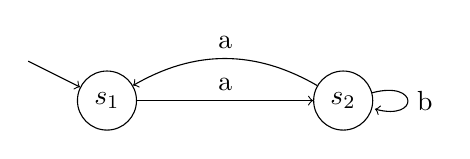
\begin{tikzpicture}[->]
			\tikzstyle{state} = [circle,draw,minimum size=0.75cm]
			
			\node[state] (s1) at (1,1.5) {$s_1$};
			\node[state] (s2) at (4,1.5) {$s_2$};
			
			\path (s1) edge node[above]{a} (s2) ;
			\path (s2) edge[bend right] node[above]{a} (s1) ;
			\path (s2) edge [loop right] node[right]{b} (s2);
			
			\path (0,2) edge (s1);
		\end{tikzpicture}
		\caption[LTS $M$]{LTS $M$}
		\label{fig:exverltsprojempty}
	\end{figure}

	The resulting parity game is depicted in Figure \ref{fig:exverpg}. Let $V$ denote the set of vertices of this parity game. There are two vertices with more than one outgoing edge. From vertex $(s_1, [a](\mu X.\phi) \vee \langle b \rangle \top)$ player 0 does not want to play to $(s_1, \langle b \rangle \top)$ because he/she will not be able to make another move and looses the path. From vertex $(s_2, [a](\mu X.\phi)  \vee \langle b \rangle \top)$ player 0 can play to $(s_2, \langle b \rangle \top)$ to bring the play in $(s_2,\top)$ to win the path. We get the following winning sets:
	\begin{align*}
	W_1 &= \{ (s_1, \langle b \rangle \top )\}\\
	W_0 &= V \backslash W_1
	\end{align*}
	With the strategies $\sigma_0$ for player $0$ and $\sigma_1$ for player $1$ being (vertices with one outgoing edge are omitted):
	\begin{align*}
	\sigma_0 = \{
	&(s_1, [a](\mu X. \phi) \vee \langle b \rangle \top) \mapsto (s_1, [a] (\mu X. \phi)), \\
	&(s_2, [a](\mu X. \phi) \vee \langle b \rangle \top) \mapsto (s_2, \langle b \rangle \top) \} \\
	\sigma_1 = \{&\}
	\end{align*}
	Note that the choice where to go from $(s_2, [a](\mu X.\phi) \vee \langle b \rangle \top)$ does not matter for the winning sets.
	\begin{figure}[h]
		\centering
		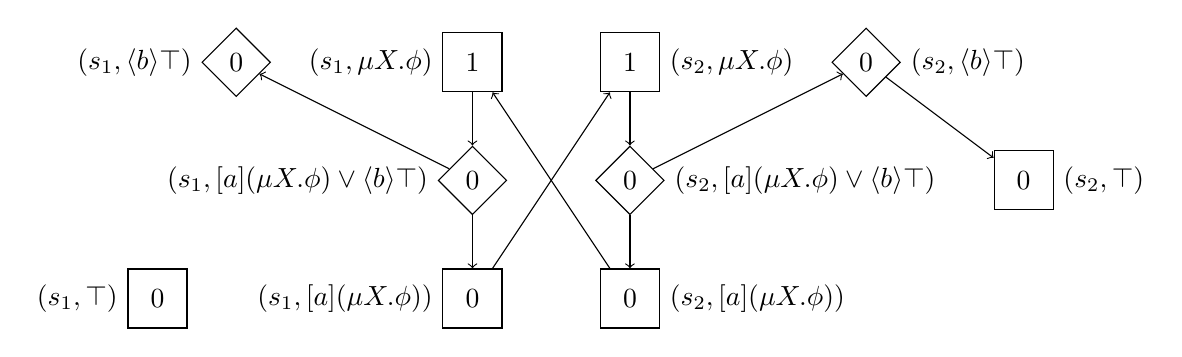
\begin{tikzpicture}[->]
			\tikzstyle{even} = [diamond,draw,minimum size=0.75cm]
			\tikzstyle{odd}  = [rectangle,draw,shape aspect=1,minimum size=0.75cm]
			
			\node[even,label={west:$(s_1,\langle b \rangle\top)$}] (s1<b>T) at (10,10) {0};
			\node[odd,label={west:$(s_1,\top)$}] (s1T) at (9,7) {0};
			
			
			\node[odd,label={west:$(s_1,\mu X.\phi)$}] (s1muxphi) at (13,10) {1};
			\node[even,label={west:$(s_1,[a](\mu X.\phi) \vee \langle b \rangle \top)$}] (s1muxphiunf) at (13,8.5) {0};
			\node[odd,label={west:$(s_1,[a](\mu X .\phi))$}] (s1[a]muxphi) at (13,7) {0};
			
			\node[odd,label={east:$(s_2,\mu X.\phi)$}] (s2muxphi) at (15,10) {1};
			\node[even,label={east:$(s_2,[a](\mu X.\phi) \vee \langle b \rangle \top)$}] (s2muxphiunf) at (15,8.5) {0};
			\node[odd,label={east:$(s_2,[a](\mu X .\phi))$}] (s2[a]muxphi) at (15,7) {0};
			
			
			\node[even,label={east:$(s_2,\langle b \rangle\top)$}] (s2<b>T) at (18,10) {0};
			\node[odd,label={east:$(s_2,\top)$}] (s2T) at (20,8.5) {0};
			
			\path (s1muxphiunf) edge (s1<b>T);
			\path (s1muxphi) edge (s1muxphiunf);
			\path (s1muxphiunf) edge (s1[a]muxphi);
			
			\path (s2muxphiunf) edge (s2<b>T);
			\path (s2muxphi) edge (s2muxphiunf);
			\path (s2muxphiunf) edge (s2[a]muxphi);
			\path (s2<b>T) edge (s2T);
			
			\path(s1[a]muxphi) edge (s2muxphi);
			\path(s2[a]muxphi) edge (s1muxphi);
		\end{tikzpicture}
		
		\caption[Parity game $LTS2PG(M, \varphi)$]{Parity game $LTS2PG(M, \varphi)$ with $\phi = [a] X \vee \langle b \rangle \top$}
		\label{fig:exverpg}
	\end{figure}
\end{example}

Parity games created in this manner relate back to the model verification question; state $s$ in LTS $M$ satisfies $\varphi$ if and only if player $0$ wins vertex $(s, \varphi)$. This is formally stated in the following theorem which is proven in \cite{Bradfield2018}.
\begin{theorem}[\cite{Bradfield2018}]
	\label{the_LTS_PG_REL}Given LTS $M = (S, Act, trans, s_0)$, modal $\mu$-calculus formula $\varphi$ and state $s \in S$ it holds that $(M, s) \models \varphi$ if and only if $(s,\varphi) \in W_0$ for the game $LTS2PG(M, \varphi)$.
\end{theorem}

\subsection{Globally and locally solving parity games}
Parity games can be solved \textit{globally} or \textit{locally}; globally solving a parity game means that for every vertex in the game it is determined who the winner is. Locally solving a parity game means that for a specific vertex in the game it is determined who the winner is. For some applications of parity games, including model checking, there is a specific vertex that needs to be solved to solve the original problem. Locally solving the parity game is sufficient in such cases to solve the original problem.

Most parity game algorithms (including the two considered next) are concerned with globally solving, when talking about solving a parity game we talk about globally solving it unless stated otherwise. 

\subsection{Parity game algorithms}
Various algorithms for solving parity games are known, we introduce two of them. First Zielonka's recursive algorithm which is well studied and generally considered to be one of the best performing parity game algorithms in practice \cite{Oink,SolvingPGInPractice}. We also inspect the fixed-point iteration algorithm which tends to perform well for model-checking problems with a low number of distinct priorities \cite{BDDSolvingPG}.

\subsubsection{Zielonka's recursive algorithm}
First we consider Zielonka's recursive algorithm \cite{ZIELONKA1998135,MCNAUGHTON1993149}, which solves total parity games. Pseudo code is presented in Algorithm \ref{alg_zlnk_org}. Zielonka's recursive algorithm has a worst-case time complexity of $O(e*n^d)$where $e$ is the number of edges, $n$ the number of vertices and $d$ the number of distinct priorities \cite{friedmanPG}.
\begin{algorithm}
	\caption{$\textsc{RecursivePG}(\textit{PG } G = (V,V_0,V_1, E, \Omega))$}
	\label{alg_zlnk_org}
	\begin{algorithmic}[1]
		\If{$V = \emptyset$}
		\State \Return $(\emptyset, \emptyset)$
		\EndIf
		\State $h \gets\max\{ \Omega(v)\ |\ v \in V\}$
		\State $\alpha \gets 0$ if $h$ is even and $1$ otherwise
		\State $U \gets \{v \in V\ |\ \Omega(v) = h\}$
		\State $A \gets \alpha\textit{-Attr}(G, U)$
		\State $(W_0', W_1') \gets \textsc{RecursivePG}(G \backslash A)$
		\If{$W_{\overline{\alpha}}' =\emptyset$}
		\State $W_\alpha \gets A \cup W_\alpha'$
		\State $W_{\overline{\alpha}} \gets \emptyset$
		\Else
		\State $B \gets \overline{\alpha}\textit{-Attr}(G,W_{\overline{\alpha}}')$
		\State $(W_0'', W_1'') \gets \textsc{RecursivePG}(G \backslash B)$
		\State $W_\alpha \gets W_\alpha''$
		\State $W_{\overline{\alpha}} \gets W_{\overline{\alpha}}'' \cup B$
		\EndIf
		\State \Return $(W_0, W_1)$
	\end{algorithmic}
\end{algorithm}

The algorithm solves $G$ by taking the set of vertices with the highest priority and choosing player $\alpha$ such that $\alpha$ has the same parity as the highest priority. Next the algorithm finds set $A$ such that player $\alpha$ can force the play to one of these high priority vertices. Next this set of vertices is removed from $G$ and the resulting subgame $G'$ is solved recursively. 

If $G'$ is entirely won by player $\alpha$ then we distinguish three cases for any path played in $G$. Either the path eventually stays in $G'$, $A$ is infinitely often visited or the path eventually stays in $A$. In the first case player $\alpha$ wins because game $G'$ was entirely won by player $\alpha$. In the second and third case player $\alpha$ can play to the highest priority from $A$. The highest priority, which has parity $\alpha$, is visited infinitely often and player $\alpha$ wins.

If $G'$ is not entirely won by player $\alpha$ we consider winning sets $W'_0$ and $W'_1$ of subgame $G'$. Vertices in set $W'_{\overline{\alpha}}$ are won by player $\overline{\alpha}$ in $G'$ but are also won by player $\overline{\alpha}$ in $G$. The algorithm tries to find all the vertices in $G$ such that player $\overline{\alpha}$ can force the play to a vertex in $W'_{\overline{\alpha}}$ and therefore winning the game. We now have a set of vertices that are definitely won by player $\overline{\alpha}$ in game $G$. In the rest of the game player $\alpha$ can keep the play from $W'_{\overline{\alpha}}$ so the algorithm solves the rest of the game recursively to find the complete winning sets for game $G$.

A complete explanation of the algorithm can be found in \cite{ZIELONKA1998135}, we do introduce definitions for the attractor set and for subgames. 

An attractor set is a set of vertices $A \subseteq V$ calculated for player $\alpha$ given set $U \subseteq V$ where player $\alpha$ has a strategy to force the play starting in any vertex in $A \backslash U$ to a vertex in $U$. Such a set is calculated by adding vertices owned by player $\alpha$ that have an edge to the attractor set and adding vertices owned by player $\overline{\alpha}$ that only have edges to the attractor set.

\begin{definition}[\cite{ZIELONKA1998135}]
	\label{def_attr}Given parity game $G = (V,V_0,V_1,E,\Omega)$ and a non-empty set $U \subseteq V$ we define $\alpha\textit{-Attr}(G,U)$ such that
	\[U_0 = U \]
	For $i \geq 0$:
	\begin{align*}
	U_{i+1} = U_i\cup
	&\{v \in V_\alpha\ |\ \exists v' \in V : v' \in U_i \wedge (v,v') \in E \}\\
	\cup &\{v \in V_{\overline{\alpha}}\ |\ \forall v' \in V :(v,v') \in E \implies v' \in U_i \}
	\end{align*}
	Finally:
	\[\alpha\textit{-Attr}(G,U) = \bigcup_{i \geq 0} U_i \]
\end{definition}

\begin{figure}
	\centering
	\begin{subfigure}{1\textwidth}
		\centering
		\begin{tikzpicture}[->]
			\tikzstyle{even} = [diamond,draw,minimum size=0.75cm]
			\tikzstyle{odd}  = [rectangle,draw,shape aspect=1,minimum size=0.75cm]
			
			\node[even] (v1) at (10,10) {1};
			\node[odd]  (v2) at (11.5,10) {3};
			\node[odd]  (v3) at (13,10) {3};
			\node[even,fill=highlightgraph] (v4) at (14.5,10) {2};
			\node[even] (v5) at (16,10) {2};
			
			\node[even] (v6) at (11.5,8.5) {1};
			\node[odd]  (v7) at (13,8.5) {0};
			\node[even,fill=highlightgraph] (v8) at (14.5,8.5) {0};
			
			\path (v1) edge [bend right] (v2);
			\path (v2) edge [bend right] (v1);
			\path (v2) edge (v3);
			\path (v3) edge (v4);
			\path (v4) edge [bend left] (v5);
			\path (v5) edge [bend left] (v4);
			
			\path (v6) edge (v1);
			\path (v2) edge (v6);
			\path (v6) edge (v3);
			\path (v7) edge (v3);
			\path (v7) edge (v8);
			\path (v3) edge (v8);
			\path (v4) edge [bend left] (v8);
			\path (v8) edge [bend left] (v4);
		\end{tikzpicture}
		\caption{Set $U = U_0$}
	\end{subfigure}\\
	\begin{subfigure}{1\textwidth}
		\centering
		\begin{tikzpicture}[->]
			\tikzstyle{even} = [diamond,draw,minimum size=0.75cm]
			\tikzstyle{odd}  = [rectangle,draw,shape aspect=1,minimum size=0.75cm]
			
			\node[even] (v1) at (10,10) {1};
			\node[odd]  (v2) at (11.5,10) {3};
			\node[odd,fill=highlightgraph]  (v3) at (13,10) {3};
			\node[even,fill=highlightgraph] (v4) at (14.5,10) {2};
			\node[even,fill=highlightgraph] (v5) at (16,10) {2};
			
			\node[even] (v6) at (11.5,8.5) {1};
			\node[odd]  (v7) at (13,8.5) {0};
			\node[even,fill=highlightgraph] (v8) at (14.5,8.5) {0};
			
			\path (v1) edge [bend right] (v2);
			\path (v2) edge [bend right] (v1);
			\path (v2) edge (v3);
			\path (v3) edge (v4);
			\path (v4) edge [bend left] (v5);
			\path (v5) edge [bend left] (v4);
			
			\path (v6) edge (v1);
			\path (v2) edge (v6);
			\path (v6) edge (v3);
			\path (v7) edge (v3);
			\path (v7) edge (v8);
			\path (v3) edge (v8);
			\path (v4) edge [bend left] (v8);
			\path (v8) edge [bend left] (v4);
		\end{tikzpicture}
		\caption{Set $U_1$}
	\end{subfigure}\\
	\begin{subfigure}{1\textwidth}
		\centering
		\begin{tikzpicture}[->]
			\tikzstyle{even} = [diamond,draw,minimum size=0.75cm]
			\tikzstyle{odd}  = [rectangle,draw,shape aspect=1,minimum size=0.75cm]
			
			\node[even] (v1) at (10,10) {1};
			\node[odd]  (v2) at (11.5,10) {3};
			\node[odd,fill=highlightgraph]  (v3) at (13,10) {3};
			\node[even,fill=highlightgraph] (v4) at (14.5,10) {2};
			\node[even,fill=highlightgraph] (v5) at (16,10) {2};
			
			\node[even,fill=highlightgraph] (v6) at (11.5,8.5) {1};
			\node[odd,fill=highlightgraph]  (v7) at (13,8.5) {0};
			\node[even,fill=highlightgraph] (v8) at (14.5,8.5) {0};
			
			\path (v1) edge [bend right] (v2);
			\path (v2) edge [bend right] (v1);
			\path (v2) edge (v3);
			\path (v3) edge (v4);
			\path (v4) edge [bend left] (v5);
			\path (v5) edge [bend left] (v4);
			
			\path (v6) edge (v1);
			\path (v2) edge (v6);
			\path (v6) edge (v3);
			\path (v7) edge (v3);
			\path (v7) edge (v8);
			\path (v3) edge (v8);
			\path (v4) edge [bend left] (v8);
			\path (v8) edge [bend left] (v4);
		\end{tikzpicture}
		\caption{Set $U_2 = 0\textit{-Attr}(G,U)$}
	\end{subfigure}
	\caption{Game $G$ showing the attractor calculation for $0\textit{-Attr}(G,U)$}
	\label{fig:AttrCalcExample}
\end{figure}
\begin{example}
	Figure \ref{fig:AttrCalcExample} shows an example parity game in which an attractor set is calculated for player $0$. For set $U_2$ no more vertices can be attracted so we found the complete attractor set.
\end{example}

The algorithm also creates subgames, where a set of vertices is removed from a parity game to create a new parity game.

\begin{definition}[\cite{ZIELONKA1998135}]
	\label{def_org_subgame}
	Given a parity game $G = (V,V_0,V_1, E,\Omega)$ and $U \subseteq V$ we define the subgame $G \backslash U$ to be the game $(V', V_0', V_1', E', \Omega)$ with:
	\begin{itemize}
		\item $V' = V \backslash U$,
		\item $V_0' = V_0 \cap V'$,
		\item $V_1' = V_1 \cap V'$ and
		\item $E' = E \cap (V' \times V')$.
	\end{itemize}
\end{definition}

Note that a subgame is not necessarily total, however the recursive algorithm always creates subgames that are total (shown in \cite{ZIELONKA1998135}).

\subsubsection{Fixed-point iteration algorithm}
Parity games can be solved by solving an alternating fixed-point formula \cite{WALUKIEWICZ2002311}. Consider PG $G = (V,V_0,V_1, E, \Omega)$ with $d$ distinct priorities. We can apply \textit{priority compression} to make sure every priority in $G$ maps to a value in $\{0,\dots,d-1\}$ or $\{1, \dots, d\}$ \cite{SolvingInPractice,FPITE}. We assume without loss of generality that the priorities map to $\{0,\dots,d-1\}$ and that $d-1$ is even. 

Consider the following formula
\[ S(G) = \nu Z_{d-1}. \mu Z_{d-2}. \dots . \nu Z_0. F_0(G,Z_{d-1},\dots,Z_0) \]
with
\begin{align*}
 F_0(G = (V,V_0,V_1,E,\Omega),Z_{d-1},\dots,Z_0) = &\{ v \in V_0\ |\ \exists_{w\in V}\ (v,w) \in E \wedge w\in Z_{\Omega(w)} \}\\
  \cup &\{ v \in V_1\ |\ \forall_{w\in V}\ (v,w) \in E \implies w\in Z_{\Omega(w)} \}
\end{align*}
where $Z_i \subseteq V$. The formula $\nu X. f(X)$ solves the greatest fixed-point of $X$ in $f$, similarly $\mu X.f(X)$ solves the least fixed-point of $X$ in $f$. As shown in \cite{WALUKIEWICZ2002311} formula $S(G)$ is calculates the set of vertices winning for player 0 in parity game $G$.

To understand the formula we consider sub-formula $\nu Z_0. F_0(Z_{d-1},\dots,Z_0)$. This formula holds for vertices from which player $0$ can either force the play into a node with priority $i > 0$ for which $Z_i$ holds or the player can stay in vertices with priority $0$ indefinitely. The formula $\mu Z_0. F_0(Z_{d-1},\dots,Z_0)$ holds for vertices from which player $0$ can force the play into a node with priority $i > 0$, for which $Z_i$ holds in finitely many steps. By alternating fixed-points the formula allows infinitely many consecutive stays in even vertices and finitely many consecutive stays in odd vertices. For an extensive treatment we refer to \cite{WALUKIEWICZ2002311}.

We further inspect formula $S$. Given game $G$, consider the following sub-formulas:
\[ S^{d-1}(Z_{d-1}) = \mu Z_{d-2}.S^{d-2}(Z_{d-2})\]
\[ S^{d-2}(Z_{d-2}) = \nu Z_{d-3}.S^{d-3}(Z_{d-3})\]
\begin{center}
	\dots
\end{center}
\[ S^{0}(Z_0) = F_0(Z_{d-1},\dots,Z_0)\]
The fixed-point variables are all elements of $2^V$, therefore we have for every sub-formula the following type:
\[ S^i(Z_i) : 2^V \rightarrow 2^V \]
Furthermore, since $V$ is finite, the partially ordered set $\langle 2^V, \subseteq \rangle$ is a complete lattice; for every subset $X \subseteq 2^V$ we have infimum $\bigcap_{x \in X} x$ and supremum $\bigcup_{x \in X} x$. Finally every sub-formula $S^i(Z_i)$ is monotonic, ie. if $S^i(Z_i) \geq S^i(Z_i')$ then $Z_i \geq Z_i'$.

Fixed-point formula's can be solved by \textit{fixed-point iteration}. As shown in \cite{Emerson:1986:MCP:900378} we can calculate $\mu X.f(X)$, where $f$ is monotonic in $X$ and $X \in 2^V$, by iterating $X$:
\[ \mu X.f(X) = \bigcup_{i \geq 0} X^i \]
where $X^i = f(X^{i-1})$ for $i > 0$ and $X^0 \subseteq \mu X.f(X)$. So picking the smallest value possible for $X_0$ will always correctly calculate $\mu X. f(X)$.

Similarly we can calculate fixed-point $\nu X.f(X)$ when $f$ is monotonic in $X$ by iterating $X$:
\[ \nu X.f(X) = \bigcap_{i \geq 0} X^i \]
where $X^i = f(X^{i-1})$ for $i > 0$ and $X^0 \supseteq \nu X.f(X)$. So picking the largest value possible for $X_0$ will always correctly calculate $\nu X. f(X)$.

Since every subformula is monotonic and maps from a value in $2^V$ to another value in $2^V$ we can apply fixed-point iteration to solve the subformula's, we choose initial values $\emptyset$ for least fixed-point variables and $V$ for greatest fixed-point variables.

An algorithm to perform the iteration is presented in \cite{FPITE} and shown in Algorithm \ref{alg_FPITEorg}. This algorithm has a worst-case time complexity of $O(e * n ^d)$ where $e$ is the number of edges, $n$ the number of vertices and $d$ the number of distinct priorities.
\begin{algorithm}
	\caption{Fixed-point iteration}
	\label{alg_FPITEorg}
	\begin{multicols}{2}
		\begin{algorithmic}[1]
			\Function{FPIter}{$G = (V, V_0, V_1, E, \Omega)$}
			\For{$i \gets d-1,\dots,0$}
			\State $\textsc{Init}(i)$
			\EndFor
			\Repeat
			\State $Z_0'\gets Z_0$
			\State $Z_0 \gets \textsc{Diamond}() \cup \textsc{Box}()$
			\State $i \gets 0$
			\While{$Z_i=Z_i' \wedge i < d-1$}
			\State $i \gets i+1$
			\State $Z_i' \gets Z_i$
			\State $Z_i \gets Z_{i-1}$
			\State $\textsc{Init}(i-1)$
			\EndWhile
			\Until{$i = d-1 \wedge Z_{d-1} = Z_{d-1}'$}
			\State \Return $(Z_{d-1},V\backslash Z_{d-1})$
			\EndFunction
		\end{algorithmic}\bigskip\bigskip
		\begin{algorithmic}[1]
			\Function{Init}{$i$}
			\State $Z_i \gets \emptyset$ if $i$ is odd, $V$ otherwise
			\EndFunction
		\end{algorithmic}\bigskip
		\begin{algorithmic}[1]
			\Function{Diamond}{}
			\State \Return $\{ v \in V_0\ |\ \exists_{w\in V} (v,w) \in E \wedge w \in Z_{\Omega(w)}\}$
			\EndFunction
		\end{algorithmic}\bigskip
		\begin{algorithmic}[1]
			\Function{Box}{}
			\State \Return $\{ v \in V_1\ |\ \forall_{w\in V} (v,w) \in E \implies w \in Z_{\Omega(w)}\}$
			\EndFunction
		\end{algorithmic}
	\end{multicols}
\end{algorithm}

\section{Symbolically representing sets}
A set can straightforwardly be represented by a collection containing all the elements that are in the set. We call this an \textit{explicit} representation of a set. We can also represent sets \textit{symbolically} in which case the set of elements is represented by some sort of formula. A typical way to represent a set symbolically is through a boolean formula encoded in a \textit{binary decision diagram} \cite{BDD_book,Handbook_BDD_Chapter}. 

\begin{example}
	\label{ex_boolform}
	The set $S = \{ 2,4,6,7 \}$ can be expressed by boolean formula:
	\[ F(x_2,x_1,x_0) = (\neg x_2 \wedge x_1 \wedge \neg x_0) \vee (x_2 \wedge (x_1 \vee \neg x_0)) \]
	where $x_0,x_1$ and $x_2$ are boolean variables. The formula gives the following truth table:\\
	\begin{center}
		\begin{tabular}{|c|c|}
			\hline 
			$\mathbf{x_2x_1x_0}$ & $\mathbf{F(x_2,x_1,x_0)}$ \\ 
			\hline 
			000 & 0 \\ 
			\hline 
			001 & 0 \\ 
			\hline 
			010 & 1 \\ 
			\hline 
			011 & 0 \\ 
			\hline 
			100 & 1 \\ 
			\hline 
			101 & 0 \\ 
			\hline 
			110 & 1 \\ 
			\hline 
			111 & 1 \\ 
			\hline
		\end{tabular} 
	\end{center}
	The function $F$ defines set $S'$ in the following way: $S' = \{x_2x_1x_0\ |\ F(x_2,x_1,x_0) = 1 \}$. As we can see set $S'$ contains the same numbers as $S$ but represented binary.
\end{example}
We can perform set operations on sets represented as boolean functions by performing logical operations on the functions. For example, given boolean formula's $f$ and $g$ representing sets $V$ and $W$ the formula $f \wedge g$ represents set $V \cap W$.

Given a set $S$ with arbitrary elements we can represent subsets $S' \subseteq S$ as boolean formula's by assigning a number to every element in $S$ and creating a boolean formula that maps boolean variables to true if and only if they represent a number such that the element associated with this number in $S$ is also in $S'$.

\subsection{Binary decision diagrams}
\label{sec_prelim_bdd}
A boolean function can efficiently be represented as a binary decision diagram (BDD), for a comprehensive treatment of BDDs we refer to \cite{BDD_book,Handbook_BDD_Chapter}.

BDDs represent boolean formula's as a directed graph where every vertex represents a boolean variable and has two outgoing edges labelled 0 and 1. Furthermore the graph contains special vertices $0$ and $1$ that have no outgoing edges. We decide if a boolean variable assignment satisfies the formula by starting in the initial vertex of the graph and following a path until we get to either vertex 0 or 1. Since every vertex represents a boolean formula we can create a path from the initial vertex by choosing edge 0 at a vertex if the boolean variable represented by that vertex is false in the variable assignment and choosing edge 1 if is true. Eventually we end up in either vertex 0 or 1. In the former case the boolean variable assignment does not satisfy the formula, in the latter it does.

\begin{example}
	Consider the boolean formula in Example \ref{ex_boolform}. This formula can be represented as the BDD shown in Figure \ref{fig:ex_simplebdd}. The vertices representing boolean variables are shown as circles and the boolean variables they represent are indicated inside them. The special vertices are represented as squares and the initial vertex is represented by an edge with that has no origin vertex.
\begin{figure}[h]
	\centering
	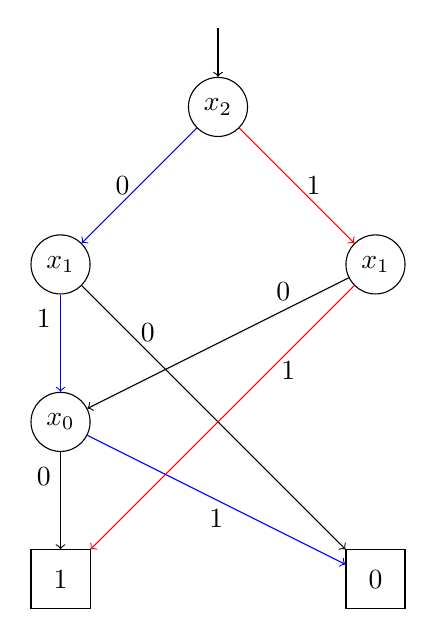
\begin{tikzpicture}[->]
		\tikzstyle{state} = [circle,draw,minimum size=0.75cm]
		\tikzstyle{final}  = [rectangle,draw,shape aspect=1,minimum size=0.75cm]
		
		\node[state] (x2) at (20,20) {$x_2$};
		\node[state] (x10) at (18,18) {$x_1$};
		\node[state] (x11) at (22,18) {$x_1$};
		\node[state] (x0) at (18,16) {$x_0$};
		\node[final] (f1) at (18,14) {$1$};
		\node[final] (f0) at (22,14) {$0$};
		
		\path (20,21) edge (x2);
		\path (x2) edge[blue] node[black,left] {0} (x10);
		\path (x2) edge[red] node[black,right] {1} (x11);
		
		\path (x10) edge[blue] node[black,left,near start] {1} (x0);
		\path (x10) edge[black] node[black,above,near start] {0} (f0);
		
		\path (x11) edge[black] node[black,above,near start] {0} (x0);
		\path (x11) edge[red] node[black,below,near start] {1} (f1);
		
		\path (x0) edge[black] node[black,left,near start] {0} (f1);
		\path (x0) edge[blue] node[black,below] {1} (f0);
	\end{tikzpicture}
	\caption{BDD highlighting boolean variable assignment $x_2x_1x_0 = 011$ in blue and $x_2x_1 = 11$ in red}
	\label{fig:ex_simplebdd}
\end{figure}
	
	The path created from variable assignment $x_2x_1x_0 = 011$ is highlighted in blue in the diagram and shows that this assignment is indeed not satisfied by the boolean formula. The red path shows the variable assignments $110$ and $111$. Determining the path and the outcome for every variable assignment results in the same truth table as seen in Example \ref{ex_boolform}.
\end{example}

Given $n$ boolean variables and two boolean functions encoded as BDDs we can perform binary operations $\vee,\wedge$ on the BDDs in $O(N_a * N_b)$, where $N_a$ and $N_b$ are the number of nodes in the decision diagrams of the two functions. A decision diagram is a tree with $n$ levels, so $N_a = O(2^n)$ and $N_b = O(2^n)$. Therefore with $n$ boolean variables we can perform binary operations $\vee$ and $\wedge$ on them in $O(2^{2n})=O(m^2)$ where $m = 2^n$ is the maximum set size that can be represented by $n$ variables \cite{BDD_running_time,Handbook_BDD_Chapter}. Since the running time specifically depends on the size of the decision diagrams, in general if the boolean functions are simple then the size of the decision diagram is also small and operations can be performed quickly.

\section{Unified parity games}
\label{sec_unified_pg}
We can consider a VPG as a PG that is the union of all its projections. We call the resulting PG the \textit{unification} of the VPG.
\begin{definition}
Given VPG $\hat{G} = (\hat{V},\hat{V}_0,\hat{V}_1, \hat{E},\hat{\Omega}, \mathfrak{C},\theta)$ we define the unification of $\hat{G}$, denoted as $\hat{G}_{\downarrow}$, as
\[  \hat{G}_{\downarrow} = \bigcup_{c\in \mathfrak{C}}\hat{G}_{|c} \]
where the union of two PGs is trivially defined as
\[ (V,V_0,V_1,E,\Omega) \cup (V',V_0',V_1',E',\Omega') = (V \cup V', V_0 \cup V_0', V_1 \cup V_1', E \cup E', \Omega \cup \Omega') \]
\end{definition}
We will use the hat decoration ($\hat{G},\hat{V},\hat{E},\hat{\Omega},\hat{W}$) when referring to a VPG and use no hat decoration when referring to a PG.

Every vertex in game $\hat{G}_{\downarrow}$ originates from a configuration and an original vertex. Therefore we can consider every vertex in a unification as a pair consisting of a vertex and a configuration, ie. $V = \mathfrak{C} \times \hat{V}$. We can consider edges in a unification similarly, ie. $E \subseteq (\mathfrak{C} \times \hat{V}) \times (\mathfrak{C} \times \hat{V})$. Note that edges don't cross configurations, ie. for every $((c,\hat{v}) , (c',\hat{v}')) \in E$ we have $c = c'$.

If we solve the PG that is the unification of a VPG we have solved the VPG, as shown in the next theorem .
\begin{theorem}
	\label{theA_solve_UVPG_is_solve_VPG}
	Given VPG $\hat{G} =  (\hat{V},\hat{V}_0,\hat{V}_1, \hat{E},\hat{\Omega}, \mathfrak{C},\theta)$. For winning sets $W_0$ and $W_1$ for game $\hat{G}_{\downarrow}$ and winning sets $\hat{W}^c_0$ and $\hat{W}^c_1$ for some configuration $c \in \mathfrak{C}$ it holds that
	\[(c,\hat{v}) \in W_\alpha \iff \hat{v} \in \hat{W}^c_\alpha  \text{, for }\alpha \in \{0,1\}  \]
	\begin{proof}
		The bi-implication is equal to  the following to implications.
		\[ (c,\hat{v}) \in W_\alpha \implies \hat{v} \in \hat{W}^c_\alpha  \text{, for }\alpha \in \{0,1\} \]
		and
		\[ (c,\hat{v}) \notin W_\alpha\implies \hat{v} \notin \hat{W}^c_\alpha \text{, for }\alpha \in \{0,1\}  \]
		
		Since the winning sets partition the game we have $\hat{v} \notin \hat{W}^c_\alpha \implies \hat{v} \in \hat{W}^c_{\overline{\alpha}}$ (similar for set $W$). Therefore it is sufficient to prove the first implication.
		
		Let $(c,\hat{v}) \in W_\alpha$, player $\alpha$ has a strategy to win game $\hat{G}_{\downarrow}$ from vertex $(c,\hat{v})$. Since $\hat{G}_{\downarrow}$ is the union of all the projections of $\hat{G}$ we can apply the same strategy to game $\hat{G}_{|c}$ to win vertex $\hat{v}$ as player $\alpha$. Because we can win $\hat{v}$ in the projection of $\hat{G}$ to $c$ we have $\hat{v} \in \hat{W}^c_\alpha$.
	\end{proof}
\end{theorem}

One of the properties of a PG is its totality; a game is total if every vertex has at least 1 outgoing vertex. Plays in a total PG will always result in an infinite path. VPGs are total, meaning that every vertex has, for every configuration $c \in \mathfrak{C}$ at least 1 outgoing vertex admitting $c$. Because VPGs are total a unified VPG is also total. For unified VPGs we can however further investigate its totality by introducing the notion of being total for every configuration. 
\begin{definition}
	A unified VPG $(V,V_0,V_1,E,\Omega)$ is total for every configuration iff for every $(c,v) \in V$ there exists a $(c,v') \in V$ such that $((c,v),(c,v')) \in E$.
\end{definition}

It follows that if a unified VPG is total then it is also total for every configuration as shown in the following lemma.
\begin{lemma}
	\label{lem_UVPG_total}
	A unified VPG $G = (V,V_0,V_1,E,\Omega)$ that is total is also total for every configuration.
	\begin{proof}
		Since $G$ is total we have for every $(c,v) \in V$ that there exists a $(c,v') \in V$ such that $((c,v),(c',v')) \in E$. Because unified VPGs don't have edges cross configurations we find that $c = c'$ and therefore $G$ is total for every configuration.
	\end{proof}
\end{lemma}

\subsubsection{Representing unified variability parity games}
Unified VPGs have a specific structure because they are the union of parity games that have the same vertices with the same owner and priority.

We can represent a set $X \subseteq (\mathfrak{C} \times \hat{V})$ as a complete function $f : \hat{V} \rightarrow 2^\mathfrak{C}$. The set $X$ and function $f$ are equivalent, denoted by the operator $=_\lambda$, iff the following relation holds:
\[ (c,\hat{v}) \in X \iff c \in f(\hat{v}) \]
We can also represent edges as a complete function $f : \hat{E} \rightarrow 2^\mathfrak{C}$. The set $E$ and function $f$ are equivalent, denoted by the operator $=_\lambda$, iff the following relation holds:
\[ ((c,\hat{v}),(c,\hat{v}')) \in E \iff c \in f(\hat{v},\hat{v}') \]
We write $\lambda^\emptyset$ to denote the function that maps every element to $\emptyset$, clearly $\lambda^\emptyset =_\lambda \emptyset$. We call using a set of pairs to represent vertices a \textit{set-wise} representation and using functions to represent vertices a \textit{function-wise} representation.


Finally we can simplify the priority function of a unified VPG, we don't actually need to create a new function that is the unification of all the projections, we can simply use the original priority assignment function because the following relation holds:
\[ \hat{\Omega}(c,\hat{v}) = \Omega(\hat{v}) \]

\section{Recursive algorithm}
We can use Zielonka's recursive algorithm to solve VPGs, to do so we will first consider a method of creating a parity game from a VPG, called \textit{unification}.
\subsection{Unified parity games}
We can create a PG from a VPG by taking all the projections of the VPG, which are PGs, and combining them into one PG by taking the union of them. We call the resulting PG the \textit{unification} of the VPG. A parity game that is the result of a unification is called a \textit{unified PG}, also any total subgame of it will be called a unified PG. A unified PG always has a VPG from which it originated.
\begin{definition}
	Given VPG $\hat{G} = (\hat{V},\hat{V}_0,\hat{V}_1, \hat{E},\hat{\Omega}, \mathfrak{C},\theta)$ we define the unification of $\hat{G}$, denoted as $\hat{G}_{\downarrow}$, as
	\[  \hat{G}_{\downarrow} = \biguplus_{c\in \mathfrak{C}}\hat{G}_{|c} \]
	where the union of two PGs is defined as
	\[ (V,V_0,V_1,E,\Omega) \uplus (V',V_0',V_1',E',\Omega') = (V \uplus V', V_0 \uplus V_0', V_1 \uplus V_1', E \uplus E', \Omega \uplus \Omega') \]
\end{definition}
We will use the hat decoration ($\hat{G},\hat{V},\hat{E},\hat{\Omega},\hat{W}$) when referring to a VPG and use no hat decoration when referring to a PG.

Every vertex in game $\hat{G}_{\downarrow}$ originates from a configuration and an original vertex. Therefore we can consider every vertex in a unification as a pair consisting of a vertex and a configuration, ie. $V = \mathfrak{C} \times \hat{V}$. We can consider edges in a unification similarly, so $E \subseteq (\mathfrak{C} \times \hat{V}) \times (\mathfrak{C} \times \hat{V})$. Note that edges don't cross configurations so for every $((c,\hat{v}) , (c',\hat{v}')) \in E$ we have $c = c'$. Figure \ref{fig:VPG2UPG} shows an example of a unification.

\begin{figure}[h]
	\centering
	\begin{subfigure}{1\textwidth}
		\centering
		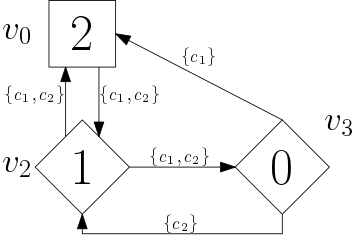
\includegraphics[scale=0.4]{Examples/UPG/VPG}
		\caption{VPG consisting of 2 configurations}
	\end{subfigure}\\
	\begin{subfigure}{1\textwidth}
		\centering
		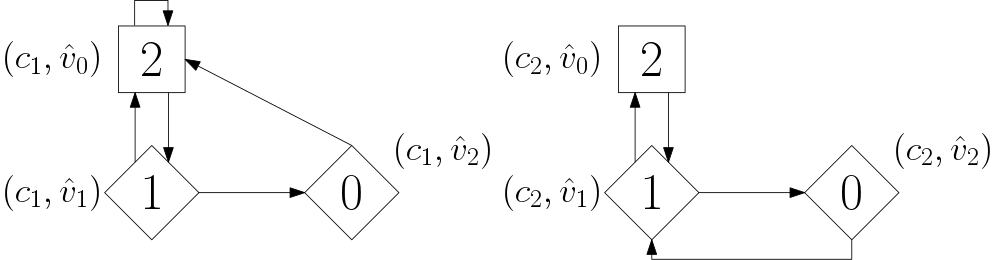
\includegraphics[scale=0.4]{Examples/UPG/UPG}
		\caption{Unified PG, created from unifying the two projections}
	\end{subfigure}
	\caption{A VPG with its corresponding unified PG}
	\label{fig:VPG2UPG}
\end{figure}

If we solve the PG that is the unification of a VPG we have solved the VPG, as shown in the next theorem.
\begin{theorem}
	\label{theA_solve_UVPG_is_solve_VPG}
	Given 
	\begin{itemize}
		\item VPG $\hat{G} =  (\hat{V},\hat{V}_0,\hat{V}_1, \hat{E},\hat{\Omega}, \mathfrak{C},\theta)$,
		\item some configuration $c \in \mathfrak{C}$,
		\item winning sets $\hat{W}^c_0$ and $\hat{W}^c_1$ for game $\hat{G}$ and
		\item winning sets $W_0$ and $W_1$ for game $\hat{G}_{\downarrow}$
	\end{itemize}
	it holds that
	\[(c,\hat{v}) \in W_\alpha \iff \hat{v} \in \hat{W}^c_\alpha  \text{, for }\alpha \in \{0,1\}  \]
	\begin{proof}
		The bi-implication is equal to  the following to implications.
		\[ (c,\hat{v}) \in W_\alpha \implies \hat{v} \in \hat{W}^c_\alpha  \text{, for }\alpha \in \{0,1\} \]
		and
		\[ (c,\hat{v}) \notin W_\alpha\implies \hat{v} \notin \hat{W}^c_\alpha \text{, for }\alpha \in \{0,1\}  \]
		
		Since the winning sets partition the game we have $\hat{v} \notin \hat{W}^c_\alpha \implies \hat{v} \in \hat{W}^c_{\overline{\alpha}}$ (similar for set $W$). Therefore it is sufficient to prove only the first implication.
		
		Let $(c,\hat{v}) \in W_\alpha$, player $\alpha$ has a strategy to win game $\hat{G}_{\downarrow}$ from vertex $(c,\hat{v})$. Since $\hat{G}_{\downarrow}$ is the union of all the projections of $\hat{G}$ we can apply the same strategy to game $\hat{G}_{|c}$ to win vertex $\hat{v}$ as player $\alpha$. Because we can win $\hat{v}$ in the projection of $\hat{G}$ to $c$ we have $\hat{v} \in \hat{W}^c_\alpha$.
	\end{proof}
\end{theorem}

\subsubsection{Projections and totality}
A unified PG can be projected back to one of the games from which it is the union.
\begin{definition}
	The projection of unified PG $G = (V,V_0, V_1,E,{\Omega})$ to configuration $c$, denoted as $G_{|c}$, is the parity game $(V',{V}_0,{V}_1,E',{\Omega})$ such that $V' = \{ {v}\ |\ (c,{v}) \in V \}$ and $E' = \{ ({v},{w})\ |\ ((c,{v}),(c,{w})) \in E \} $.
\end{definition}

One of the properties of a PG is its totality; a game is total if every vertex has at least 1 outgoing vertex. VPGs are also total, meaning that every vertex has, for every configuration $c \in \mathfrak{C}$, at least 1 outgoing vertex admitting $c$. Because VPGs are total their unifications are also total. Since edges in a unified PG don't cross configurations we can conclude that a unified PG is total iff every projection is total.

\subsection{Solving unified PGs}
We can solve a unified PG using the Zielonka's recursive algorithm. The algorithm revolves around the attractor operation and the creation of subgames. Consider the example presented in figure \ref{fig:VPG2UPG}. Vertices with the highest priority are 
\[ \{(c_1,v_0),(c_2,v_0)\}\]
attracting these for player $0$ gives the set 
\begin{align*}
\{(c_1,v_0),&(c_2,v_0),\\
(c_1,v_1),&(c_2,v_1),\\
 &(c_2,v_2)\}
\end{align*}
The algorithm tries to attract all vertices starting from $v_0$ with any configuration, in this case $v_1$ can be attracted for all configurations, $v_2$ can only be attracted for $c_2$. When edge guards are permissive, ie. they admit many configurations, then there is a good change that vertices can be attracted for multiple configurations at the same time during the algorithm. This is the idea for the family based recursive VPG algorithm we represent next, we will use the recursive algorithm to solve unified parity games such that it tries to attract multiple configurations simultaneously.

\subsection{Representing unified parity games}
In order to create an algorithm based around attracting multiple configurations we need to take a look at how unified parity games can be represented.


Unified PGs have a specific structure because they are the union of PGs that have the same vertices with the same owner and priority. Because they have the same priority we don't actually need to create a new function that is the unification of all the projections, we can simply use the original priority assignment function because the following relation holds:
\[ \Omega(c,\hat{v}) = \hat{\Omega}(\hat{v}) \]
Similarly we can use the original partition sets $\hat{V}_0$ and $\hat{V}_1$ instead of having the new partition $V_0$ and $V_1$ because the following relations holds:
\[ (c,\hat{v}) \in V_0 \iff \hat{v}\in \hat{V}_0 \]
\[ (c,\hat{v}) \in V_1 \iff \hat{v}\in \hat{V}_1 \]
So instead of considering unified PG $(V,V_0,V_1,E,\Omega)$ we will consider $(V,\hat{V}_0,\hat{V}_1,E,\hat{\Omega})$. 

Next we consider how we represent vertices and edges in a unified PG. A set $X \subseteq (\mathfrak{C} \times \hat{V})$ can be represented as a complete function $f : \hat{V} \rightarrow 2^\mathfrak{C}$. The set $X$ and function $f$ are equivalent, denoted by the operator $=_\lambda$, iff the following relation holds:
\[ (c,\hat{v}) \in X \iff c \in f(\hat{v}) \]
We can also represent edges as a complete function $f : \hat{E} \rightarrow 2^\mathfrak{C}$. The set $E$ and function $f$ are equivalent, denoted by the operator $=_\lambda$, iff the following relation holds:
\[ ((c,\hat{v}),(c,\hat{v}')) \in E \iff c \in f(\hat{v},\hat{v}') \]
We write $\lambda^\emptyset$ to denote the function that maps every element to $\emptyset$, clearly $\lambda^\emptyset =_\lambda \emptyset$. We call using a set of pairs to represent vertices and edges a \textit{set-wise} representation and using functions a \textit{function-wise} representation.

\subsection{Algorithms}
Using the recursive algorithm as a basis we can solve a VPG product based, alternatively we can solve it family based using a set-wise presentation or a function-wise presentation. For the function-wise presentation we can either use an explicit or a symbolic representation of sets of configurations. The following diagram shows the different algorithms:
\begin{center}
	\begin{forest}
		[Recursive algorithm, for tree={parent anchor=south, child anchor=north, align=center, s sep=5mm}
		[Product based]
		[Family based
		[Set-wise]
		[Function-wise
		[Explicit]
		[Symbolic]
		]
		]
		]
	\end{forest}
\end{center}

\subsection{Recursive algorithm using a function-wise representation}
We can modify the recursive algorithm to work with the function-wise representation of vertices and edges. Pseudo code for the modified algorithm is presented in algorithm \ref{alg_zlnk_UVPG}.
\begin{algorithm}
	\caption{$\textsc{recursiveUVPG}(\textit{PG } G = (\\
		V : \hat{V} \rightarrow 2^\mathfrak{C},\\
		\hat{V}_0 \subseteq \hat{V},\\
		\hat{V}_1 \subseteq \hat{V},\\
		E : \hat{E} \rightarrow 2^\mathfrak{C},\\
		\hat{\Omega} : \hat{V}\rightarrow \mathbb{N}$}\label{alg_zlnk_UVPG}
	\begin{algorithmic}[1]
		\State $m \gets \min\{ \hat{\Omega}(\hat{v})\ |\ V(\hat{v}) \neq \emptyset \}$
		\State $h \gets \max\{ \hat{\Omega}(\hat{v})\ |\ V(\hat{v}) \neq \emptyset \}$
		\If{$h = m$ or $V = \lambda^\emptyset$}
		\If{$h$ is even or $V = \lambda^\emptyset$}
		\State \Return $(V,\lambda^\emptyset)$
		\Else
		\State \Return $(\lambda^\emptyset, V)$
		\EndIf
		\EndIf
		\State $\alpha \gets 0$ if $h$ is even and $1$ otherwise
		\State $U \gets \lambda^\emptyset$, $U(\hat{v}) \gets V(\hat{v})$ for all $\hat{v}$ with $\hat{\Omega}(\hat{v}) = h$
		\State $A \gets \alpha\textit{-FAttr}(G, U)$
		\State $(W_0', W_1') \gets \textsc{recursiveUVPG}(G \backslash A)$
		\If{$W_{\overline{\alpha}}' =\lambda^\emptyset$}
		\State $W_\alpha \gets A \cup W_\alpha'$
		\State $W_{\overline{\alpha}} \gets \lambda^\emptyset$
		\Else
		\State $B \gets \overline{\alpha}\textit{-FAttr}(G,W_{\overline{\alpha}}')$
		\State $(W_0'', W_1'') \gets \textsc{recursiveUVPG}(G \backslash B)$
		\State $W_\alpha \gets W_\alpha''$
		\State $W_{\overline{\alpha}} \gets W_{\overline{\alpha}}'' \cup B$
		\EndIf
		\State \Return $(W_0, W_1)$
	\end{algorithmic}
\end{algorithm}

We introduce a modified attractor definition to work with the function-wise representation.
\begin{definition}
		\label{def_Uattr}Given unified PG $G = (V, \hat{V}_0,\hat{V}_1,E,\hat{\Omega})$ and a non-empty set $U \subseteq V$, both represented function-wise, we define $\alpha\textit{-FAttr}(G,U)$ such that
	\[U_0 = U \]
	For $i \geq 0$:
	\[
	U_{i+1}(\hat{v}) = U_i(\hat{v}) \cup \begin{cases}
V(\hat{v}) \cap \bigcup_{\hat{v}'} (E(\hat{v},\hat{v}') \cap U_i(\hat{v}')) & \text{if } \hat{v} \in \hat{V_{\alpha}}\\
V(\hat{v}) \cap \bigcap_{\hat{v'}}((\mathfrak{C} \backslash E(\hat{v},\hat{v}')) \cup U_i(\hat{v}') & \text{if }\hat{v} \in  \hat{V_{\overline{\alpha}}} \\
	\end{cases}
	\]
	Finally:
	\[\alpha\textit{-FAttr}(G,U) = \bigcup_{i \geq 0} U_i \]
\end{definition}
We will now prove that the function-wise attractor definition gives a result equal to the original definition.
\begin{lemma}
	\label{lem_attr_equal}
	Given unified PG $G = (\mathcal{V},\hat{V}_0,\hat{V}_1, \mathcal{E}, \hat{\Omega})$ and set $\mathcal{U} \subseteq \mathcal{V}$ the function-wise attractor $\alpha\textit{-FAttr}(G,\mathcal{U})$ is equivalent to the set-wise attractor $\alpha\textit{-Attr}(G,\mathcal{U})$ for any $\alpha \in \{0,1\}$.
	\begin{proof}
		Let $V,E,U$ be the set-wise representation and $V^\lambda,E^\lambda,U^\lambda$ be the function-wise representation of $\mathcal{V},\mathcal{E},\mathcal{U}$ respectively.
		
		The following properties hold by definition:
		\[ (c,\hat{v}) \in V \iff c \in V^\lambda(\hat{v})\]
		\[ (c,\hat{v}) \in U \iff c \in U^\lambda(\hat{v})\]
		\[ ((c,\hat{v}),(c,\hat{v}')) \in E \iff c \in E^\lambda(\hat{v},\hat{v}') \]
		
		Since the attractors are inductively defined and $U_0 =_\lambda U^\lambda_0$ (because $U =_\lambda U^\lambda$) we have to prove that for some $i \geq 0$, with $U_i =_\lambda U^\lambda_i$,  we have $U_{i+1} =_\lambda U^\lambda_{i+1}$, which holds iff:
		\[ (c,\hat{v}) \in U_{i+1} \iff c \in U^\lambda_{i+1}(\hat{v}) \]
		Let $(c,\hat{v}) \in V$ (and therefore $c \in V^\lambda(\hat{v})$), we consider 4 cases.
		\begin{itemize}
			\item Case: $\hat{v} \in \hat{V}_{\alpha}$ and $(c,\hat{v}) \in U_{i+1}$:\\
			To prove: $c \in U^\lambda_{i+1}(\hat{v})$.
			
			If $(c,\hat{v}) \in U_i$ then $c \in U^\lambda_i(\hat{v})$ and therefore $c \in U^\lambda_{i+1}(\hat{v})$. If $(c,\hat{v}) \notin U_i$ then we have $c \notin U^\lambda_i(\hat{v})$.
			
			
			Because $\hat{v} \in \hat{V}_{\alpha}$ and $c \in V^\lambda(\hat{v})$ we get
			\[ U^\lambda_{i+1} =\bigcup_{\hat{v}'} (E^\lambda(\hat{v},\hat{v}') \cap U^\lambda_i(\hat{v}')) \]
			
			There exists an $(c',\hat{v}') \in V$ such that $(c',\hat{v}') \in U_i$ and $((c,\hat{v}),(c',\hat{v}')) \in E$. Because edges don't cross configurations we can conclude that $c' = c$. Due to equivalence we have $c \in U^\lambda_i(\hat{v}')$ and $c \in E^\lambda(\hat{v},\hat{v}')$. If we fill this in in the above formula we can conclude that $c \in U^\lambda_{i+1}(\hat{v})$.
			\item Case: $\hat{v} \in \hat{V}_{\alpha}$ and $(c,\hat{v}) \notin U_{i+1}$:\\
			To prove: $c \notin U^\lambda_{i+1}(\hat{v})$.
			
			
			First we observe that since $(c, \hat{v}) \notin U_{i+1}$ we get $(c, \hat{v}) \notin U_{i}$ and therefore $c \notin U^\lambda_i(\hat{v})$.
			
			Because $\hat{v} \in \hat{V}_{\alpha}$ and $c \in V^\lambda(\hat{v})$ we get
\[ U^\lambda_{i+1} =\bigcup_{\hat{v}'} (E^\lambda(\hat{v},\hat{v}') \cap U^\lambda_i(\hat{v}')) \]
			
			Assume $c \in U^\lambda_{i+1}(\hat{v})$. There must exist a $\hat{v}'$ such that $c \in E^\lambda(\hat{v},\hat{v}')$ and $c \in U^\lambda_i(\hat{v}')$. Due to equivalence we have a vertex $((c,\hat{v}),(c,\hat{v}')) \in E$ and $(c,\hat{v}') \in U_i$. In which case $(c,\hat{v})$ would be attracted and would be in $U_{i+1}$ which is a contradiction.
			\item Case: $\hat{v} \in \hat{V}_{\overline{\alpha}}$ and $(c,\hat{v}) \in U_{i+1}$:\\
			To prove: $c \in U^\lambda_{i+1}(\hat{v})$.
			
			If $(c,\hat{v}) \in U_i$ then $c \in U^\lambda_i(\hat{v})$ and therefore $c \in U^\lambda_{i+1}(\hat{v})$. If $(c,\hat{v}) \notin U_i$ then we have $c \notin U^\lambda_i(\hat{v})$.
			
			Because $\hat{v} \in \hat{V}_{\overline{\alpha}}$ we get
			\[ U^\lambda_{i+1} =V^\lambda(\hat{v}) \cap \bigcap_{\hat{v'}}((\mathfrak{C} \backslash E^\lambda(\hat{v},\hat{v}')) \cup U^\lambda_i(\hat{v}') \]
			
			Assume $c \notin U^\lambda_{i+1}(\hat{v})$. Because $c \in V^\lambda(\hat{v})$ there must exist an $\hat{v}$ such that
			\[ c \notin ((\mathfrak{C} \backslash E^\lambda(\hat{v},\hat{v}')) \text{ and } c \notin U^\lambda_i(\hat{v}') \]
			which is equal to
			\[ c \in E^\lambda(\hat{v},\hat{v}') \text{ and } c \notin U^\lambda_i(\hat{v}') \]
			By equivalence we have $((c,\hat{v}),(c,\hat{v}')) \in E$ and $(c,\hat{v}') \notin U_i$. Which means that $(c,\hat{v})$ will not be attracted and $(c,\hat{v}) \notin U_{i+1}$ which is a contradiction.
			\item Case: $\hat{v} \in \hat{V}_{\overline{\alpha}}$ and $(c,\hat{v}) \notin U_{i+1}$:\\
			To prove: $c \notin U^\lambda_{i+1}(\hat{v})$.
			
			First we observe that since $(c, \hat{v}) \notin U_{i+1}$ we get $(c, \hat{v}) \notin U_{i}$ and therefore $c \notin U^\lambda_i(\hat{v})$.
			
			Because $\hat{v} \in \hat{V}_{\overline{\alpha}}$ we get
			\[ U^\lambda_{i+1} =V^\lambda(\hat{v}) \cap \bigcap_{\hat{v'}}((\mathfrak{C} \backslash E^\lambda(\hat{v},\hat{v}')) \cup U^\lambda_i(\hat{v}') \]
			
			Since $(c,\hat{v})$ is not attracted there must exist a $(c,\hat{v}') \in V$ such that 
			\[ ((c,\hat{v}),(c,\hat{v}')) \in E  \text{ and } (c,\hat{v}') \notin U_i \]
			By equivalence we have 
			\[ c \in E^\lambda(\hat{v},\hat{v}')  \text{ and } c \notin U^\lambda_i(\hat{v}') \]
			Which is equal to
			\[ c \notin (\mathfrak{C} \backslash E^\lambda(\hat{v},\hat{v}'))  \text{ and } c \notin U^\lambda_i(\hat{v}') \]
			From which we conclude
			\[ c \notin ((\mathfrak{C} \backslash E^\lambda(\hat{v},\hat{v}')) \cup U^\lambda_i(\hat{v}'))) \]
			Therefore we have $c \notin U^\lambda_{i+1}(\hat{v})$.
		\end{itemize}
	\end{proof}
\end{lemma}

We also introduce a modified subgame definition to work with the function-wise representation.
\begin{definition}
	\label{def_Usubgame}
	For unified PG $G = (V,\hat{V}_0,\hat{V}_1,E,\hat{\Omega})$, represented function-wise, and set $X \subseteq V$ we define the subgame $G \backslash X = (V',\hat{V}_0,\hat{V}_1,E',\hat{\Omega})$ such that:
	\begin{itemize}
		\item $V'(\hat{v}) = V(\hat{v}) \backslash X(\hat{v})$
		\item $E'(\hat{v},\hat{v}') = E(\hat{v},\hat{v}') \cap V'(\hat{v}) \cap V'(\hat{v}')$
	\end{itemize}
\end{definition}
We will now prove that this new subgame definition gives a result equal to the original subgame definition. Note that when using the original subgame definition for unified PGs we can omit the modification to the partition because, as we have seen, we can use the partitioning from the VPG in the representation of unified PGs.
\begin{lemma}
	\label{lem_subgame_eq}
	Given unified PG $G = (\mathcal{V},\hat{V}_0,\hat{V}_1, \mathcal{E}, \hat{\Omega})$ and set $\mathcal{U} \subseteq \mathcal{V}$ the subgame $G \backslash \mathcal{U} = (\mathcal{V}',\hat{V}_0,\hat{V}_1,\mathcal{E}',\hat{\Omega})$ represented set-wise is equal to the subgame represented function-wise.
	\begin{proof}
		Let $V,V',E,E',U$ be the set-wise and $V^\lambda,{V^\lambda}', E^\lambda, {E^\lambda}', U^\lambda$ the function-wise representations of $\mathcal{V},\mathcal{V}', \mathcal{E}, \mathcal{E}', \mathcal{U}$ respectively. We know $V =_\lambda V^\lambda$, $E =_\lambda E^\lambda$ and $U =_\lambda U^\lambda$. To prove: $V' =_\lambda {V^\lambda}'$ and $E' =_\lambda {E^\lambda}'$.
		
		Let $(c,\hat{v}) \in V$.
		
		If $(c,\hat{v}) \in U$ then $c \in U^\lambda(\hat{v})$, also $(c,\hat{v}) \notin V'$ (by definition \ref{def_org_subgame}) and $c \notin {V^\lambda}'(\hat{v})$ (by definition \ref{def_Usubgame}).
		
		If $(c,\hat{v}) \notin U$ then $c \notin U^\lambda(\hat{v})$, also $(c,\hat{v}) \in V'$ (by definition \ref{def_org_subgame}) and $c \in {V^\lambda}'(\hat{v})$ (by definition \ref{def_Usubgame}).
		
		Let $((c,\hat{v}),(c,\hat{w})) \in E$.
		
		If $(c,\hat{v}) \in U$ then $(c,\hat{v}) \notin V'$ and $c \notin {V^\lambda}'(\hat{v})$ (as shown above). We get $((c,\hat{v}),(c,\hat{w})) \notin V' \times V'$ so $((c,\hat{v}),(c,\hat{w})) \notin E'$ (by definition \ref{def_org_subgame}). Also $c \notin {E^\lambda}'(\hat{v},\hat{w})$ (by definition \ref{def_Usubgame}).
		
		If $(c,\hat{w}) \in U$ then we apply the same logic.
		
		If neither is in $U$ then both are in $V'$ and in $V' \times V'$ and therefore the $((c,\hat{v}),(c,\hat{w})) \in E'$. Also we get $c \in {V^\lambda}'(\hat{v})$ and $c \in {V^\lambda}'(\hat{w})$ so we get $c \in {E^\lambda}'(\hat{v},\hat{w})$ (by definition \ref{def_Usubgame}).
	\end{proof}
\end{lemma}

Next we prove the correctness of the algorithm by showing that the winning sets of the function-wise algorithm are equal to the winning sets of the set-wise algorithm.
\begin{theorem}
	Given unified PG $\mathcal{G} = (\mathcal{V},\hat{V}_0,\hat{V}_1, \mathcal{E}, \hat{\Omega})$ the winning sets resulting from \textsc{recursiveUVPG($\mathcal{G}$)} ran over the function-wise representation of $\mathcal{G}$ is equal to the winning sets resulting from \textsc{RecursivePG($\mathcal{G}$)} ran over the set-wise representation of $\mathcal{G}$.
	\begin{proof}
		Let $G = (V,\hat{V}_0,\hat{V}_1,E,\hat{\Omega})$ be the set-wise representation of $\mathcal{G}$ and $G^\lambda = (V^\lambda, \hat{V}_0, \hat{V}_1, E^\lambda, \hat{\Omega})$ be the function-wise representation of $\mathcal{G}$.
		
		Proof by induction on $\mathcal{G}$.
		
		\textbf{Base} When there are no vertices or only one priority \textsc{RecursiveUVPG($G^\lambda$)} returns $\lambda^\emptyset$ and \textsc{RecursivePG($G$)} returns $\emptyset$, these two results are equal therefore the theorem holds in this case.
		
		\textbf{Step}
		Player $\alpha$ gets the same value in both algorithms since the highest priority is equal for both algorithms.
		
		Let $U = \{(c,\hat{v}) \in V\ |\ \hat{\Omega}(\hat{v}) = h \}$ (as calculated by \textsc{RecursivePG}) and $U^\lambda(\hat{v}) = V^\lambda(\hat{v})$ for all $\hat{v}$ with $\hat{\Omega}(\hat{v}) = h$ (as calculated by \textsc{RecursiveUVPG}). We will show that $U =_\lambda U^\lambda$.
		
		Let $(c,\hat{v}) \in U$ then $\hat{\Omega}(\hat{v}) = h$, therefore $U^\lambda(\hat{v}) = V^\lambda(\hat{v})$. Since $U \subseteq V$ we have $(c,\hat{v}) \in V$ and because the equality between $V$ and $V^\lambda$ we get $c \in V^\lambda(\hat{v})$ and $c \in U^\lambda(\hat{V})$.
		
		Let $c \in U^\lambda(\hat{v})$, since $U^\lambda(\hat{v})$ is not empty we have $\hat{\Omega}(\hat{v}) = h$, furthermore $c \in V^\lambda(\hat{v})$ and therefore $(c,\hat{v}) \in V$. We can conclude that $(c, \hat{v}) \in U$ and $U =_\lambda U^\lambda$.
		
		For the rest of the algorithm it is sufficient to see that attractor sets are equal if the game and input set are equal (as shown in lemma \ref{lem_attr_equal}) and that the created subgames are equal (as shown in lemma \ref{lem_subgame_eq}). Since the subgames are equal we can apply the theorem on it by induction and conclude that the winning sets are also equal.
	\end{proof}
\end{theorem}

We have seen in theorem \ref{theA_solve_UVPG_is_solve_VPG} that solving a unified PG solves the VPG, furthermore the algorithm \textsc{RecursiveUVPG} correctly solves a unified PG therefore we can now conclude that for VPG $\hat{G}$ vertex $\hat{v}$ is won by player $\alpha$ for configuration $c$ iff $c \in W_\alpha(\hat{v})$ with $(W_0,W_1) = \textsc{RecursiveUVPG}(G_{\downarrow})$.

\subsubsection{Function-wise attractor set}
Next we present an algorithm to calculate the function-wise attractor, the pseudo code is presented in algorithm \ref{alg_fattr_alg}. The algorithm considers vertices that are in the attracted set for some configuration, for every such vertex the algorithm tries to attract vertices that are connected by an incoming edge. If a vertex is attracted for some configuration then the incoming edges of that vertex will also be considered. We prove the correctness of the algorithm in the following lemma and theorem.
\begin{algorithm}
	\caption{$\textsc{$\alpha$-FAttractor}(G, A : \hat{V} \rightarrow 2^\mathfrak{C})$}\label{alg_fattr_alg}
	\begin{algorithmic}[1]
		\State Queue $Q \gets \{\hat{v} \in \hat{V} \ |\ A(\hat{v}) \neq \emptyset  \}$
		\While{$Q$ is not empty}
		\State $\hat{v}' \gets Q.pop()$
		\For{$E(\hat{v},\hat{v}') \neq \emptyset$}
			\If{$\hat{v} \in \hat{V}_\alpha$}
				\State $a \gets V(\hat{v}) \cap E(\hat{v},\hat{v}') \cap A(\hat{v}')$
			\Else
				\State $a \gets V(\hat{v})$
				\For{$E(\hat{v},\hat{v}'') \neq \emptyset$}
					\State $a \gets a \cap (\mathfrak{C}\backslash E(\hat{v},\hat{v}'') \cup A(\hat{v}''))$
				\EndFor
			\EndIf
			\If{$a \backslash A(\hat{v}) \neq \emptyset$}
				\State $A(\hat{v}) \gets A(\hat{v}) \cup a$
				\State $Q.push(\hat{v})$
			\EndIf
		\EndFor
		\EndWhile
		\State \Return $A$
	\end{algorithmic}
\end{algorithm}
\begin{lemma}
\label{lem_attr_requires_E}
Vertex $\hat{v}$ and configuration $c$, with $c \in V(\hat{v})$, can only be attracted if there is a vertex $\hat{v}'$ such that $c \in E(\hat{v}, \hat{v}')$ and $c \in U_i(\hat{v}')$.
	\begin{proof}
		We first observe that if $\hat{v} \in \hat{V}_\alpha$ then this property follows immediately from definition the function-wise attractor definition (\ref{def_Uattr}). If $\hat{v} \in \hat{V}_{\overline{\alpha}}$ we note that unified PGs are total and therefore all of their projections are also total. So vertex $\hat{v}$ has at least one outgoing edge for $c$, we have $\hat{w}$ such that $c \in E(\hat{v},\hat{w})$. For $\hat{v}$ with $c$ to be attracted we must have $c \in U_i(\hat{w})$.
	\end{proof}
\end{lemma}
\begin{theorem}
Set $A$ calculated by $\textsc{$\alpha$-FAttractor}(G,U)$ satisfies $A = \alpha\textit{-FAttr}(G,U)$.
	\begin{proof} We will prove two loop invariants over the while loop of the algorithm.
		
		\textbf{IV1}: For every $\hat{w} \in \hat{V}$ and $c \in \mathfrak{C}$ with $c \in A(\hat{w})$ we have $c \in \alpha\textit{-FAttr}(G,U)(\hat{w})$.
		
		\textbf{IV2}: For every $\hat{w} \in \hat{V}$ and $c \in \mathfrak{C}$ that can be attracted to $A$ either $c \in A(\hat{w})$ or there exists a $\hat{w}' \in Q$ such that $c \in E(\hat{w},\hat{w}')$.
		
		\textbf{Base}: Before the loop starts we have $A = U$, therefore IV1 holds. Furthermore all the vertices that are in $A$ for some $c$ are also in $Q$ so IV2 holds.
		
		\textbf{Step}: Consider the beginning of an iteration and assume IV1 and IV2 hold. To prove: IV1 and IV2 hold at the end of the iteration.
		
		Set $A$ only contains vertices with configurations that are in $\alpha\textit{-FAttr}(G,U)$. The set is only updated through lines 5-12 and 14 of the algorithm which reflects the exact definition of the attractor set therefore IV1 holds at the end of the iteration.
		
		Consider $\hat{w} \in \hat{V}$ and $c \in \mathfrak{C}$, we distinguish three cases to prove IV2:
		\begin{itemize}
			\item $\hat{w}$ with $c$ can be attracted by the beginning of the iteration but not by the end.
			
			This case can't happen because $A(\hat{w})$ only increases during the algorithm and the values for $E$ and $V$ are not changed throughout the algorithm.
			\item $\hat{w}$ with $c$ can't be attracted by the beginning of the iteration but can by the end.
			
			For $\hat{w}$ with $c$ to be able to be attracted at the end of the iteration there must be some $\hat{w}'$ with $c$ such that during the iteration $c$ was added to $A(\hat{w}')$ (lemma \ref{lem_attr_requires_E}). Every $\hat{w}'$ for which $A(\hat{w}')$ is updated is added to the queue (lines 13-16). Therefore we have $\hat{w}' \in Q$ with $c \in E(\hat{w},\hat{w}')$ and IV1 holds.
			\item $\hat{w}$ with $c$ can be attracted by the beginning of the iteration and also by the end.
			
			Since IV2 holds at the beginning of the iteration we have either $c \in A(\hat{w})$ or we have some $\hat{w}' \in Q$ such that $c \in E(\hat{w},\hat{w}')$. In the former case IV2 holds trivially by the end of the iteration since $A(\hat{w})$ can only increase. For the latter case we distinguish two scenario's. 
			
			First we consider the scenario where vertex $\hat{v}'$ that is considered during the iteration (line 3 of the algorithm) is $\hat{w}'$. There is a vertex $c \in E(\hat{w},\hat{w}')$ by IV2. Therefore we can conclude that $\hat{w}$ is considered in the for loop starting at line $4$ and will be attracted in lines 5-12 and added to $A(\hat{w})$ in line 14. Therefore IV2 holds by the end of the iteration.
			
			Next we consider the scenario where $\hat{v}' \neq \hat{w}'$. In this case by the end of the iteration $\hat{w}'$ will still be in $Q$ and IV2 holds.
		\end{itemize}
	
	Vertices are only added to the queue when something is added to $A$ (if statement on line 13). This can only finitely often happen because $A(\hat{v})$ can never be larger than $V(\hat{v})$ so we can conclude that the while loop terminates after a finite number of iterations.
	
		When the while loop terminates IV1 and IV2 hold so for every $\hat{w} \in \hat{V}$ and $c \in \mathfrak{C}$ that can be attracted to $A$ we have $c \in A(\hat{w})$. Since we start with $A = U$ we can conclude the soundness of the algorithm. IV1 shows the completeness.
	\end{proof}
\end{theorem}


\subsection{Running time}
We will consider the running time for solving VPG $G = (V,V_0,V_1,E,\Omega,\mathfrak{C},\theta)$ product based and family based using the different types of representations. We will use $n$ to denote the number of vertices, $e$ the number of edges, $c$ the number of configurations and $d$ the number of distinct priorities.

The original algorithm runs in $O(e * n^d)$, if we run $c$ parity games independently we get $O(c * e * n ^d)$. We can also apply the original algorithm to a unified PG (represented set-wise) for a family based approach, in this case we get a parity game with $c*n$ vertices and $c*e$ edges. which gives a running time $O(c*e*(c*n)^d)$. However this running time can be improved by using the property that a unified PG consists of $c$ disconnected graphs as we shown next.

We have introduced three types of family based algorithms: set-wise, function-wise with explicit configuration sets and function-wise with symbolic configuration sets. In all three algorithms the running time of the attractor set is dominant, so we need three things: analyse the running time of the base cases, analyse the running time of the attractor set and analyse the recursion.

\textit{Base cases.} In the base cases the algorithm needs to do two things: find the highest and lowest priority and check if there are no more vertices in the game. For the set-wise variant we find the highest and lowest priorities by iterating all vertices, which takes $O(c*n)$. Checking if there are no more vertices is done in $O(1)$. For the function wise algorithms we can find the highest and lowest priority in $O(n)$ and checking if there are no vertices is also done in $O(n)$ since we have to check $V(\hat{v}) = \emptyset$ for every $\hat{v}$. Note that in a symbolic representation using BDDs we can check if a set is empty in $O(1)$ because the decision diagram contains a single node.

\textit{Attractor sets.} For the set-wise family based approach we can use the attractor calculation from the original algorithm which has a time complexity of $O(e)$, so for a unified PG having $c*e$ edges we have $O(c*e)$.

The function-wise variants use a different attractor algorithm. First we consider the variant where sets of configurations are represented explicitly.

Consider algorithm \ref{alg_fattr_alg}. A vertex will be added to the queue when this vertex is attracted for some configuration, this can only happen $c*n$ times, once for every vertex configuration combination. 

The first for loop considers all the incoming edges of a vertex. When we consider all vertices the for loop will have considered all edges, since we consider every vertex at most $c$ times the for loop will run at most $c*e$ times in total.

The second for loop considers all outgoing edges of a vertex. The vertices that are considered are the vertices that have an edge going to the vertex being considered by the while loop. Since the while loop considers $c*n$ vertices the second for loop runs in total at most $c * n * e$ times. The loop itself performs set operations on the set of configurations which can be done in $O(c)$. This gives a total time complexity for the attractor set of $O(n*c^2*e)$.

For the symbolic representation set operations can be done in $O(c^2)$ so we get a time complexity of $O(n*c^3*e)$.

This gives the following time complexities\\
\begin{center}
	\begin{tabular}{|c|c|c|}
		\hline 
		& Base & Attractor set \\ 
		\hline 
		Set-wise & $O(c*n)$ & $O(c*e)$  \\ 
		\hline 
		Function-wise explicit & $O(n)$ &  $O(n*c^2*e)$ \\ 
		\hline 
		Function-wise symbolic & $O(n)$ &  $O(n* c^3*e)$ \\ 
		\hline 
	\end{tabular} 
\end{center}

\textit{Recursion}. The three algorithms behave the same way with regards to their recursion, so we analyse the running time of the set-wise variant and can derive the time complexity of the others using the result.

The algorithm has two recursions, the first recursion lowers the number of distinct priorities by 1. The second recursion removes at least one edge, however the game is comprised of disjoint projections. We can use this fact use in the analyses. Consider unified PG $G$ and $A$ as specified by the algorithm. Now consider the projection of $G$ to an arbitrary configuration $q$, $G_{|q}$. If $(G\backslash A)_{|q}$ contains a vertex that is won by player $\overline{\alpha}$ then this vertex is removed in the second recursion step. If there is no vertex won by player $\overline{\alpha}$ then the game is won in its entirety and the only vertices won by player $\overline{\alpha}$ are in different projections. We can conclude that for every configuration $q$ the second recursion either removes a vertex or $(G\backslash A)_{|q}$ is entirely won by player $\alpha$. Let $\overline{n}$ denote be the maximum number of vertices that are won by player $\overline{\alpha}$ in game $(G\backslash A)_{|q}$. Since every projection has at most $n$ vertices the value for $\overline{n}$ can be at most $n$. Furthermore since $\overline{n}$ depends on $A$, which depends on the maximum priority, the value $\overline{n}$ gets reset when the top priority is removed in the first recursion. We can now write down the recursion of the algorithm:
\[ T(d,\overline{n}) \leq T(d-1,n) + T(d, \overline{n} - 1) + O(c*e) \]
When $\overline{n} = 0$ we will get $W_{\overline{\alpha}} = \emptyset$ as a result of the first recursion. In such a case there will be only 1 recursion.
\[ T(d,0) \leq T(d-1,n) + O(c*e) \]
Finally we have the base case where there is 1 priority:
\[ T(1, \overline{n}) \leq O(c*n) \]
Expanding the second recursion gives
\begin{align*}
T(d) &\leq (n+1)T(d-1) + (n+1)O(c*e)\\
T(1) &\leq O(c*n)
\end{align*}
We will now prove that $T(d) \leq (n+d)^dO(c*e)$ by induction on $d$.

\textbf{Base} $d=1$: $T(1) \leq O(c*n) \leq O(c*e) \leq (n+1)^1O(c*e)$

\textbf{Step} $d > 1$:
\begin{align*}
T(d) &\leq (n+1)T(d-1) + (n+1)O(c*e)\\
&\leq (n+1)(n+d-1)^{d-1}O(c*e) + (n+1)O(c*e)
\end{align*}
Since $n+1 \leq n+d-1$ we get:
\begin{align*}
T(d) &\leq (n+d-1)(n+d-1)^{d-1}O(c*e) + (n+1)O(c*e)\\
&\leq (n+d-1)^dO(c*e) + (n+1)O(c*e)\\
&\leq ((n+d-1)^d + n + 1)O(c*e)
\end{align*}
Using lemma \ref{lem_md_ineq} we get
\begin{align*}
T(d) &\leq (n+d)^dO(c*e)
\end{align*}
This gives a time complexity of $O(c*e*(n+d)^d) = O(c*e*n^d)$. Note that the base time complexity is subsumed in the recursion by the time complexity of the attractor set. Since the time complexity of the attractor set is higher that the time complexity of the base cases for all three variants of algorithms we can simply fill in the attractor time complexity to get $O(n*c^2*e*n^d)$ for the function-wise explicit algorithm and $O(n*c^3*e*n^d)$ for the function-wise symbolic algorithm.

The different algorithms, including their time complexities, are repeated in the diagram below:\\
\begin{center}
	\begin{forest}
	[Recursive algorithm, for tree={parent anchor=south, child anchor=north, align=center, s sep=5mm}
		[Product based\\$O(c*e*n^d)$ ]
		[Family based
			[Set-wise\\$O(c*e*n^d)$ ]
			[Function-wise
				[Explicit\\$O(n * c^2 * e * n^d)$ ]
				[Symbolic\\$O(n * c^3 * e * n^d)$ ]
			]
		]
	]
	\end{forest}
\end{center}

The function wise time complexities consist of three parts:
\begin{itemize}
	\item the number of edges in the queue during the attractor calculation,
	\item the time complexity of set operations on subsets of $\mathfrak{C}$ and
	\item the number of recursions.
\end{itemize}
The number of vertices in the queue during attracting is at most $c*n$, however this number will only be large if we attract a very small number of configurations at a per time we evaluate an edge. Most likely we will be able to attract many configurations at the same time, especially when the VPG originates from an FTS there is a good change that many edges admit most or all configurations in $\mathfrak{C}$. So when there are many similarities in behaviour between the different configurations in the FTS we will have a low number of vertices in the queue.

The time complexity of set operations is $O(c)$ when using an explicit representation and $O(c^2)$ when using a symbolic one. However, as shown in \cite{BDD_running_time}, a breadth-depth first implementation of BDDs keeps a table of already computed results. This allows us to get already calculated results in sublinear time. In total there are $2^c$ possible sets and therefore $2^{2c}$ possible set combinations and $O(2^c)$ possible set operations that can be computed. However when solving a VPG originating from an FTS there will most likely be a relatively small number of different edge guards, in which case the number of unique sets considered in the algorithm will be small and we can often retrieve a set calculation from the computed table.

We can see that even though the running time of the family based symbolic algorithm is the worse, its actual running time might be good when we are able to attract multiple configurations at the same time and have a small number of different edge guards.

\section{Pessimistic parity games}
Given a VPG with configurations $\mathfrak{C}$ we can try to determine sets $P_0,P_1$ such that the vertices in set $P_\alpha$ are won by player $\alpha \in \{0,1\}$ for any configuration in $\mathfrak{C}$. We can do so by creating a \textit{pessimistic} PG; a pessimistic PG is a parity game created from a VPG for a player $\alpha \in \{0,1\}$ such that the PG allows all edges that player $\overline{\alpha}$ might take but only allows edges for $\alpha$ when that edge admits all the configurations in $\mathfrak{C}$.
\begin{definition}
	\label{def_pess_game}
	Given VPG $G = (V,V_0,V_1,E,\Omega, \mathfrak{C},\theta)$, we can create pessimistic PG $G_{\triangleright\alpha}$ for player $\alpha \in \{0,1\}$. We have	
	\[ G_{\triangleright\alpha} = \{V,V_0,V_1,E',\Omega \} \]
	such that
	\[ E' = \{ (v,w) \in E\ |\ v \in V_{\overline{\alpha}} \vee \theta(v,w) = \mathfrak{C} \} \]
\end{definition}


Note that pessimistic parity games are not necessarily total. A play in a PG that is not total might result in a finite path, in such a case the player that can't make a move looses the play.

When solving a pessimistic PG $G_{\triangleright\alpha}$ we get winning sets $W_0,W_1$, every vertex in $W_\alpha$ is winning for player $\alpha$ in $G$ played for any configuration, as shown in the following theorem.
\begin{theorem}
	\label{the_pess_is_winning_for_all_conf}
	Given:
	\begin{itemize}
		\item VPG $G = (V,V_0,V_1,E,\Omega,\mathfrak{C},\theta)$,
		\item configuration $c \in \mathfrak{C}$,
		\item winning sets $W_0^c, W_1^c$ for game $G$,
		\item player $\alpha \in \{0,1\}$ and
		\item pessimistic PG $G_{\triangleright\alpha}$ with winning sets $P_0$ and $P_1$
	\end{itemize}
we have $P_\alpha \subseteq W_\alpha^c$.
	\begin{proof}
		Player $\alpha$ has a strategy in game $G_{\triangleright\alpha}$ such that vertices in $P_\alpha$ are won. We will show that this strategy can also be applied to game $G_{|c}$ to win the same or more vertices.
		
		First we observe that any edge that is taken by player $\alpha$ in game $G_{\triangleright\alpha}$ can also be taken in game $G_{|c}$ so player $\alpha$ can play the same strategy in game $G_{|c}$.
		
		For player $\overline{\alpha}$ there are possibly edges that can be taken in $G_{\triangleright\alpha}$ but can't be taken in $G_{|c}$, in such a case player $\overline{\alpha}$'s choices are limited in game $G_{|c}$ compared to $G_{\triangleright\alpha}$ so if player $\overline{\alpha}$ can't win a vertex in $G_{\triangleright\alpha}$ then he/she can't win that vertex in $G_{|c}$.
		
		We can conclude that applying the strategy from game $G_{\triangleright\alpha}$ in game $G_{|c}$ for player $\alpha$ wins the same or more vertices.
	\end{proof}
\end{theorem}
Figure \ref{fig:VPG2PPGs} shows an example VPG with corresponding pessimistic games, after solving the pessimistic games we find $P_0 = \{v_2\}$ and $P_1 = \{v_0\}$.
\begin{figure}[h]
	\centering
	\begin{subfigure}{1\textwidth}
		\centering
		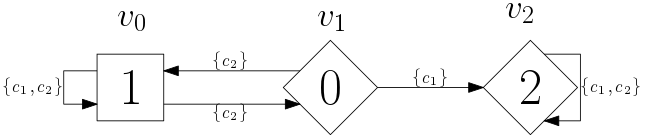
\includegraphics[scale=0.4]{Examples/PPG/VPG}
		\caption{VPG $G$ consisting of 2 configurations}
	\end{subfigure}\\
	\begin{subfigure}{1\textwidth}
		\centering
		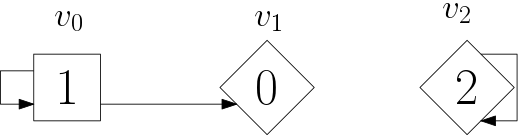
\includegraphics[scale=0.4]{Examples/PPG/P0}
		\caption{Pessimistic game $G_{\triangleright0}$}
	\end{subfigure}\\
	\begin{subfigure}{1\textwidth}
		\centering
		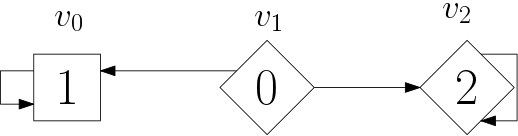
\includegraphics[scale=0.4]{Examples/PPG/P1}
		\caption{Pessimistic game $G_{\triangleright1}$}
	\end{subfigure}
	\caption{A VPG with its corresponding pessimistic games}
	\label{fig:VPG2PPGs}
\end{figure}
\subsection{Configuration partitioning}
We can create a sub-VPG from a VPG by only considering a part of the configurations from the original VPG.
\begin{definition}
	Given VPG $G = (V,V_0,V_1,E,\Omega,\mathfrak{C},\theta)$ and non-empty set $\mathfrak{X} \subseteq \mathfrak{C}$ we define the subgame $G \cap \mathfrak{X} = (V,V_0,V_1,E',\Omega,\mathfrak{C}', \theta')$ such that
	\begin{itemize}
		\item $\mathfrak{C}' =\mathfrak{C} \cap \mathfrak{X}$,
		\item $\theta'(e) = \theta(e) \cap \mathfrak{C}'$ and
		\item $E' = \{ e \in E\ |\ \theta'(e) \neq \emptyset \}$.
	\end{itemize}
\end{definition}
VPGs are total, meaning that for every configuration and every vertex there is an outgoing edge from that vertex admitting that configuration. In subgames the set of configurations is restricted and only edge guards and edges are removed for configurations that fall outside the restricted set, therefore we still have totality.

Furthermore it is trivial to see that every projection $G_{|c}$ is equal to $(G \cap \mathfrak{X})_{|c}$ for any $c \in \mathfrak{C} \cap \mathfrak{X}$.

Finally the subgame operator is associative, meaning $(G \cap \mathfrak{X}) \cap \mathfrak{X}' = G \cap (\mathfrak{X} \cap \mathfrak{X}') = G \cap \mathfrak{X} \cap \mathfrak{X}'$.

Vertices in winning set $P_\alpha$ for $G_{\triangleright\alpha}$ are also winning for player $\alpha$ in pessimistic subgames of $G$, as shown in the following lemma.
\begin{lemma}
	\label{lem_pessimistic_subgames}
	Given:
	\begin{itemize}
		\item VPG $G = (V,V_0,V_1,E,\Omega, \mathfrak{C},\theta)$,
		\item $P_0$ being the winning set of game $G_{\triangleright0}$ for player $0$,
		\item $P_1$ being the winning set of game $G_{\triangleright1}$ for player $1$,
		\item non-empty set $\mathfrak{X} \subseteq \mathfrak{C}$,
		\item player $\alpha \in \{0,1\}$ and
		\item winning sets $Q_0,Q_1$ for game $(G \cap \mathfrak{X})_{\triangleright\alpha}$
	\end{itemize}
	we have
	\[ P_0 \subseteq Q_0 \]
	\[ P_1 \subseteq Q_1 \]
	\begin{proof}
	
		Let edge $(v,w)$ be an edge in game $G_{\triangleright\alpha}$ with $v \in V_\alpha$. Edge $(v,w)$ admits all configuration in $\mathfrak{C}$ so it also admits all configuration in $\mathfrak{C} \cap \mathfrak{X}$, therefore we can conclude that edge $(v,w)$ is also an edge of game $(G\cap \mathfrak{X})_{\triangleright\alpha}$.
		
		Let edge $(v,w)$ be an edge in game $(G \cap \mathfrak{X})_{\triangleright\alpha}$ with $v \in V_{\overline{\alpha}}$. The edge admits some configuration in $\mathfrak{C} \cap \mathfrak{X}$, this configuration is also in $\mathfrak{C}$ so we can conclude that edge $(v,w)$ is also an edge of game $G_{\triangleright\alpha}$.
		
		We have concluded that game $(G \cap \mathfrak{X})_{\triangleright\alpha}$ has the same or more edges for player $\alpha$ as game $G_{\triangleright\alpha}$ and the same or less edges for player $\overline{\alpha}$. Therefore we can conclude that any vertex won by player $\alpha$ in $G_{\triangleright\alpha}$ is also won by $\alpha$ in game $(G \cap \mathfrak{X})_{\triangleright\alpha}$, ie. $P_\alpha \subseteq Q_\alpha$.
		
		
		Let $v \in P_{\overline{\alpha}}$, using theorem \ref{the_pess_is_winning_for_all_conf} we find that $v$ is winning for player $\overline{\alpha}$ in $G_{|c}$ for any $c \in \mathfrak{C}$. Because projections of subgames are the same as projections of the original game we can conclude that $v$ is winning for player $\overline{\alpha}$ in $(G \cap \mathfrak{X})_{|c}$ for any $c \in \mathfrak{C} \cap \mathfrak{X}$.
		
		Assume $v \notin Q_{\overline{\alpha}}$ then $v \in Q_{\alpha}$ and using theorem \ref{the_pess_is_winning_for_all_conf} we find that $v$ is winning for player $\alpha$ in $(G \cap \mathfrak{X})_{|c}$ for any $c \in \mathfrak{C} \cap \mathfrak{X}$. This is a contradiction so we can conclude $v \in Q_{\overline{\alpha}}$ and therefore $P_{\overline{\alpha}} \subseteq Q_{\overline{\alpha}}$.
	\end{proof}
\end{lemma}


\section{Incremental pre-solve algorithm}
Next we explore an algorithm where we try to solve the game for all configurations as much as possible, then split the configurations in two sets, create subgames using those two configuration sets and recursively repeat the process. Specifically we try to find vertices that are won by the same player for all configurations in $\mathfrak{C}$, if we have a vertex that is won by the same player for all configurations we say such a vertex is pre-solved. The algorithm tries to recursively the set of pre-solved vertices until all vertices are either pre-solved or only 1 configuration remains. Pseudo code is presented in algorithm \ref{alg_IncPreSolveBasic}. The algorithm is based around finding sets $P_0$ and $P_1$, furthermore we want to find these sets in a clever such that the algorithm doesn't spend time finding vertices that are already pre-solved. Furthermore when there is only 1 configuration left we want an algorithm that solves the parity game $G_{|c}$ in an efficient manner by using the vertices that are pre-solved.

\begin{algorithm}
	\caption{$\textsc{IncPreSolve}(G = (V,V_0,V_1, E, \Omega, \mathfrak{C}, \theta), P_0,P_1)$}\label{alg_IncPreSolveBasic}
	\begin{algorithmic}[1]
		\If{$|\mathfrak{C}| = 1$}
		\State $\{c\} \gets \mathfrak{C}$
		\State $(W'_0,W'_1) \gets $ solve $G_{|c}$ using $P_0$ and $P_1$
		\State \Return $(\mathfrak{C} \times W'_0, \mathfrak{C} \times W'_1)$
		\EndIf
		\State $P'_0 \gets$ find vertices won by player $0$ for all configuration in $\mathfrak{C}$
		\State $P'_1 \gets$ find vertices won by player $1$ for all configuration in $\mathfrak{C}$
		\If{$P'_0 \cup P'_1 = V$}
		\State \Return $(\mathfrak{C} \times P'_0, \mathfrak{C} \times P'_1)$
		\EndIf
		\State $\mathfrak{C}^a, \mathfrak{C}^b \gets $ partition $\mathfrak{C}$ in non-empty parts
		\State $(W_0^a, W_1^a) \gets \textsc{IncPreSolve}(G \cap \mathfrak{C}^a, P'_0,P'_1)$
		\State $(W_0^b, W_1^b) \gets \textsc{IncPreSolve}(G \cap \mathfrak{C}^b, P'_0,P'_1)$
		\State $W_0 \gets W_0^a \cup W_0^b$
		\State $W_1 \gets W_1^a \cup W_1^b$
		\State \Return $(W_0,W_1)$
	\end{algorithmic}
\end{algorithm}
The subgames created are based on creating a subgame based on a set of configurations, we define the subgame operator as follows:
\begin{definition}
	Given VPG $G = (V,V_0,V_1,E,\Omega,\mathfrak{C},\theta)$ and non-empty set $\mathfrak{X} \subseteq \mathfrak{C}$ we define the subgame $G \cap \mathfrak{X} = (V,V_0,V_1,E',\Omega,\mathfrak{C}', \theta')$ such that
	\begin{itemize}
		\item $\mathfrak{C}' =\mathfrak{C} \cap \mathfrak{X}$,
		\item $\theta'(e) = \theta(e) \cap \mathfrak{C}'$ and
		\item $E' = \{ e \in E\ |\ \theta'(e) \neq \emptyset \}$.
	\end{itemize}
\end{definition}
VPGs are total, meaning that for every configuration and every vertex there is an outgoing edge from that vertex admitting that configuration. In subgames the set of configurations is restricted and only edge guards and edges are removed for configurations that fall outside the restricted set, therefore we still have totality.

Furthermore it is trivial to see that every projection $G_{|c}$ is equal to $(G \cap \mathfrak{X})_{|c}$ for any $c \in \mathfrak{C} \cap \mathfrak{X}$.

Finally the subgame operator is associative, meaning $(G \cap \mathfrak{X}) \cap \mathfrak{X}' = G \cap (\mathfrak{X} \cap \mathfrak{X}') = G \cap \mathfrak{X} \cap \mathfrak{X}'$.

\subsection{Finding $P_0$ and $P_1$}
We can find $P_0$ and $P_1$ by using \textit{pessimistic} parity games; a pessimistic PG is a parity game created from a VPG for a player $\alpha \in \{0,1\}$ such that the PG allows all edges that player $\overline{\alpha}$ might take but only allows edges for $\alpha$ when that edge admits all the configurations in $\mathfrak{C}$.
\begin{definition}
	\label{def_pess_game}
	Given VPG $G = (V,V_0,V_1,E,\Omega, \mathfrak{C},\theta)$, we can create pessimistic PG $G_{\triangleright\alpha}$ for player $\alpha \in \{0,1\}$. We have	
	\[ G_{\triangleright\alpha} = \{V,V_0,V_1,E',\Omega \} \]
	such that
	\[ E' = \{ (v,w) \in E\ |\ v \in V_{\overline{\alpha}} \vee \theta(v,w) = \mathfrak{C} \} \]
\end{definition}


Note that pessimistic parity games are not necessarily total. A play in a PG that is not total might result in a finite path, in such a case the player that can't make a move looses the play.

When solving a pessimistic PG $G_{\triangleright\alpha}$ we get winning sets $W_0,W_1$, every vertex in $W_\alpha$ is winning for player $\alpha$ in $G$ played for any configuration, as shown in the following theorem.
\begin{theorem}
	\label{the_pess_is_winning_for_all_conf}
	Given:
	\begin{itemize}
		\item VPG $G = (V,V_0,V_1,E,\Omega,\mathfrak{C},\theta)$,
		\item configuration $c \in \mathfrak{C}$,
		\item winning sets $W_0^c, W_1^c$ for game $G$,
		\item player $\alpha \in \{0,1\}$ and
		\item pessimistic PG $G_{\triangleright\alpha}$ with winning sets $P_0$ and $P_1$
	\end{itemize}
	we have $P_\alpha \subseteq W_\alpha^c$.
	\begin{proof}
		Player $\alpha$ has a strategy in game $G_{\triangleright\alpha}$ such that vertices in $P_\alpha$ are won. We will show that this strategy can also be applied to game $G_{|c}$ to win the same or more vertices.
		
		First we observe that any edge that is taken by player $\alpha$ in game $G_{\triangleright\alpha}$ can also be taken in game $G_{|c}$ so player $\alpha$ can play the same strategy in game $G_{|c}$.
		
		For player $\overline{\alpha}$ there are possibly edges that can be taken in $G_{\triangleright\alpha}$ but can't be taken in $G_{|c}$, in such a case player $\overline{\alpha}$'s choices are limited in game $G_{|c}$ compared to $G_{\triangleright\alpha}$ so if player $\overline{\alpha}$ can't win a vertex in $G_{\triangleright\alpha}$ then he/she can't win that vertex in $G_{|c}$.
		
		We can conclude that applying the strategy from game $G_{\triangleright\alpha}$ in game $G_{|c}$ for player $\alpha$ wins the same or more vertices.
	\end{proof}
\end{theorem}
Figure \ref{fig:VPG2PPGs} shows an example VPG with corresponding pessimistic games, after solving the pessimistic games we find $P_0 = \{v_2\}$ and $P_1 = \{v_0\}$.
\begin{figure}[h]
	\centering
	\begin{subfigure}{1\textwidth}
		\centering
		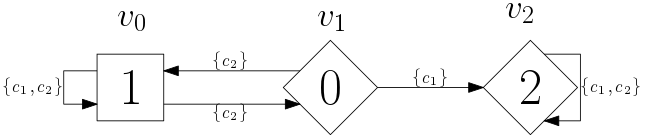
\includegraphics[scale=0.4]{Examples/PPG/VPG}
		\caption{VPG $G$ consisting of 2 configurations}
	\end{subfigure}\\
	\begin{subfigure}{1\textwidth}
		\centering
		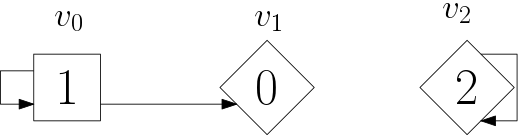
\includegraphics[scale=0.4]{Examples/PPG/P0}
		\caption{Pessimistic game $G_{\triangleright0}$}
	\end{subfigure}\\
	\begin{subfigure}{1\textwidth}
		\centering
		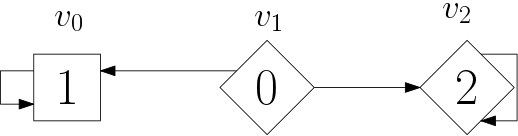
\includegraphics[scale=0.4]{Examples/PPG/P1}
		\caption{Pessimistic game $G_{\triangleright1}$}
	\end{subfigure}
	\caption{A VPG with its corresponding pessimistic games}
	\label{fig:VPG2PPGs}
\end{figure}
\subsubsection{Pessimistic subgames}
Vertices in winning set $P_\alpha$ for $G_{\triangleright\alpha}$ are also winning for player $\alpha$ in pessimistic subgames of $G$, as shown in the following lemma.
\begin{lemma}
	\label{lem_pessimistic_subgames}
	Given:
	\begin{itemize}
		\item VPG $G = (V,V_0,V_1,E,\Omega, \mathfrak{C},\theta)$,
		\item $P_0$ being the winning set of game $G_{\triangleright0}$ for player $0$,
		\item $P_1$ being the winning set of game $G_{\triangleright1}$ for player $1$,
		\item non-empty set $\mathfrak{X} \subseteq \mathfrak{C}$,
		\item player $\alpha \in \{0,1\}$ and
		\item winning sets $Q_0,Q_1$ for game $(G \cap \mathfrak{X})_{\triangleright\alpha}$
	\end{itemize}
	we have
	\[ P_0 \subseteq Q_0 \]
	\[ P_1 \subseteq Q_1 \]
	\begin{proof}
		
		Let edge $(v,w)$ be an edge in game $G_{\triangleright\alpha}$ with $v \in V_\alpha$. Edge $(v,w)$ admits all configuration in $\mathfrak{C}$ so it also admits all configuration in $\mathfrak{C} \cap \mathfrak{X}$, therefore we can conclude that edge $(v,w)$ is also an edge of game $(G\cap \mathfrak{X})_{\triangleright\alpha}$.
		
		Let edge $(v,w)$ be an edge in game $(G \cap \mathfrak{X})_{\triangleright\alpha}$ with $v \in V_{\overline{\alpha}}$. The edge admits some configuration in $\mathfrak{C} \cap \mathfrak{X}$, this configuration is also in $\mathfrak{C}$ so we can conclude that edge $(v,w)$ is also an edge of game $G_{\triangleright\alpha}$.
		
		We have concluded that game $(G \cap \mathfrak{X})_{\triangleright\alpha}$ has the same or more edges for player $\alpha$ as game $G_{\triangleright\alpha}$ and the same or less edges for player $\overline{\alpha}$. Therefore we can conclude that any vertex won by player $\alpha$ in $G_{\triangleright\alpha}$ is also won by $\alpha$ in game $(G \cap \mathfrak{X})_{\triangleright\alpha}$, ie. $P_\alpha \subseteq Q_\alpha$.
		
		
		Let $v \in P_{\overline{\alpha}}$, using theorem \ref{the_pess_is_winning_for_all_conf} we find that $v$ is winning for player $\overline{\alpha}$ in $G_{|c}$ for any $c \in \mathfrak{C}$. Because projections of subgames are the same as projections of the original game we can conclude that $v$ is winning for player $\overline{\alpha}$ in $(G \cap \mathfrak{X})_{|c}$ for any $c \in \mathfrak{C} \cap \mathfrak{X}$.
		
		Assume $v \notin Q_{\overline{\alpha}}$ then $v \in Q_{\alpha}$ and using theorem \ref{the_pess_is_winning_for_all_conf} we find that $v$ is winning for player $\alpha$ in $(G \cap \mathfrak{X})_{|c}$ for any $c \in \mathfrak{C} \cap \mathfrak{X}$. This is a contradiction so we can conclude $v \in Q_{\overline{\alpha}}$ and therefore $P_{\overline{\alpha}} \subseteq Q_{\overline{\alpha}}$.
	\end{proof}
\end{lemma}
\subsection{Algorithm}
In order to find $P_0$ and $P_1$ we need to solve a pessimistic parity game, specifically we want to solve a parity game that uses the vertices that are already pre-solved to efficiently solve the parity game. Note that when there is 1 configuration left we need a similar algorithm. In algorithm \ref{alg_FPITE} we present the \textsc{IncPreSolve} algorithm using pessimistic parity games. The algorithm uses a \textsc{Solve} algorithm for solving parity games using the pre-solved vertices. First we will show the correctness of the algorithm, later we will explore an appropriate \textsc{Solve} algorithm.
\begin{algorithm}
	\caption{$\textsc{IncPreSolve}(G = (V,V_0,V_1, E, \Omega, \mathfrak{C}, \theta), P_0,P_1)$}\label{alg_IncPreSolve}
	\begin{algorithmic}[1]
		\If{$|\mathfrak{C}| = 1$}
		\State $\{c\} \gets \mathfrak{C}$
		\State $(W'_0,W'_1) \gets \textsc{Solve}(G_{|c}, P_0,P_1)$
		\State \Return $(\mathfrak{C} \times W'_0, \mathfrak{C} \times W'_1)$
		\EndIf
		\State $(P'_0,-) \gets \textsc{Solve}(G_{\triangleright0}, P_0, P_1)$
		\State $(-,P'_1) \gets \textsc{Solve}(G_{\triangleright1}, P_0, P_1)$
		\If{$P'_0 \cup P'_1 = V$}
		\State \Return $(\mathfrak{C} \times P'_0, \mathfrak{C} \times P'_1)$
		\EndIf
		\State $\mathfrak{C}^a, \mathfrak{C}^b \gets $ partition $\mathfrak{C}$ in non-empty parts
		\State $(W_0^a, W_1^a) \gets \textsc{IncPreSolve}(G \cap \mathfrak{C}^a, P'_0,P'_1)$
		\State $(W_0^b, W_1^b) \gets \textsc{IncPreSolve}(G \cap \mathfrak{C}^b, P'_0,P'_1)$
		\State $W_0 \gets W_0^a \cup W_0^b$
		\State $W_1 \gets W_1^a \cup W_1^b$
		\State \Return $(W_0,W_1)$
	\end{algorithmic}
\end{algorithm}

A \textsc{Solve} algorithm must correctly solve a game as long as the sets $P_0$ and $P_1$ are in fact vertices that are won by player $0$ and $1$ respectively. We prove that this is the case in the \textsc{IncPreSolve} algorithm.
\begin{theorem}
	Given VPG $\hat{G}$. For every $\textsc{Solve}(G,P_0,P_1)$ that is invoked during $\textsc{IncPreSolve}(\hat{G},\emptyset,\emptyset)$ we have winning sets $W_0,W_1$ for game $G$ for which the following holds:
	\[ P_0 \subseteq  W_0 \]
	\[ P_1 \subseteq  W_1 \]
	\begin{proof}
		When $P_0 = \emptyset$ and $P_1 = \emptyset$ the theorem holds trivially. So we will start the analyses after the first recursion. 
		
		After the first recursion the game is $\hat{G} \cap \mathfrak{X}$ with $\mathfrak{X}$ being either $\mathfrak{C}^a$ or $\mathfrak{C}^b$. The set $P_0$ is the winning set for player $0$ for game $\hat{G}_{\triangleright0}$ and the set $P_1$ is the winning set for player $1$ for game $\hat{G}_{\triangleright1}$. In the next recursion the game is $\hat{G} \cap \mathfrak{X} \cap \mathfrak{X}'$ with $P_0$ being the winning set for player $0$ in game $(\hat{G} \cap \mathfrak{X})_{\triangleright0}$ and $P_1$ being the winning set for player $1$ in game $(\hat{G} \cap \mathfrak{X})_{\triangleright1}$. In general, after the $k$th recursion, with $k > 0$, the game is of the form  $(\hat{G} \cap \mathfrak{X}^0 \cap \dots \cap \mathfrak{X}^{k-1}) \cap \mathfrak{X}^k$. Furthermore $P_0$ is the winning set for player $0$ for game $(\hat{G} \cap \mathfrak{X}^0 \cap \dots \cap \mathfrak{X}^{k-1})_{\triangleright0}$ and $P_1$ is the winning set for player $1$ for game $(\hat{G} \cap \mathfrak{X}^0 \cap \dots \cap \mathfrak{X}^{k-1})_{\triangleright1}$.
		
		Next we inspect the three places \textsc{Solve} is invoked:
		\begin{enumerate}
			\item Consider the case where there is only one configuration in $\mathfrak{C}$ (line 1-5). Because $P_0$ is the winning set for player $0$ for game $(\hat{G} \cap \mathfrak{X}^0 \cap \dots \cap \mathfrak{X}^{k-1})_{\triangleright0}$ the vertices in $P_0$ are won by player $0$ in game $G_{|c}$ for all $c \in \mathfrak{X}^0 \cap \dots \cap \mathfrak{X}^{k-1}$ (using theorem \ref{the_pess_is_winning_for_all_conf}). This includes the one element in $\mathfrak{C}$. So we can conclude $P_0 \subseteq W_0$ where $W_0$ is the winning set for player $0$ in game $G_{|c}$ where $\{c\} = \mathfrak{C}$.
			
			Similarly for player $1$ we can conclude $P_1 \subseteq W_1$ and the theorem holds in this case.
			\item On line $6$ the game $G_{\triangleright0}$ is solved with $P_0$ and $P_1$. Because $G = \hat{G} \cap \mathfrak{X}^0 \cap \dots \cap \mathfrak{X}^{k-1} \cap \mathfrak{X}^k$ and $P_0$ is the winning set for player $0$ for game $(\hat{G} \cap \mathfrak{X}^0 \cap \dots \cap \mathfrak{X}^{k-1})_{\triangleright0}$ and $P_1$ is the winning set for player $1$ for game $(\hat{G} \cap \mathfrak{X}^0 \cap \dots \cap \mathfrak{X}^{k-1})_{\triangleright1}$ we can apply lemma \ref{lem_pessimistic_subgames} to conclude that the theorem holds in this case.
			\item On line $7$ we apply the same reasoning and lemma to conclude that the theorem holds in this case.
		\end{enumerate}
	\end{proof}
\end{theorem}

Next we prove the correctness of the algorithm, assuming the correctness of the \textsc{Solve} algorithm.
\begin{theorem}
	%TODO hat notatie
	Given VPG $\hat{G} = (\hat{V},\hat{V}_0,\hat{V}_1,\hat{E},\hat{\Omega},\mathfrak{C},\theta)$ and $(W_0,W_1) = \textsc{IncPreSolve}(\hat{G},\emptyset,\emptyset)$. For every configuration $c \in \mathfrak{C}$ and winning sets $\hat{W}_0^c, \hat{W}_1^c$ for game $\hat{G}$ player for $c$ it holds that:
	\[ (c,v) \in W_0 \iff v \in \hat{W}_0^c \]
	\[ (c,v) \in W_1 \iff v \in \hat{W}_1^c \]
	\begin{proof}
		We will prove the theorem by applying induction on $\mathfrak{C}$.
		
		\textbf{Base} $|\mathfrak{C}| = 1$, when there is only one configuration, being $c$, then the algorithm solves game $G_{|c}$. The product of the winning sets and $\{c\}$ is returned, so the theorem holds.
		
		\textbf{Step} Consider $P_0'$ and $P_1'$ as calculated in the algorithm (line 6-7). By theorem \ref{the_pess_is_winning_for_all_conf} all vertices in $P_0'$ are won by player $0$ in game $G_{|c}$ for any $c \in \mathfrak{C}$, similarly for $P_1'$ and player $1$.
		
		If $P_0' \cup P_1' = V$ then the algorithm returns $(\mathfrak{C} \times P_0',\mathfrak{C} \times P_1')$. In which case the theorem holds because there are no configuration vertex combinations that are not in either winning set and theorem \ref{the_pess_is_winning_for_all_conf} proves the correctness.
		
		If $P_0' \cup P_1' \neq V$ then we have winning sets $(W_0^a, W_1^a)$ for which the theorem holds (by induction) for game $G \cap \mathfrak{C}^a$ and $(W_0^b, W_1^b)$ for which the theorem holds (by induction) for game $G \cap \mathfrak{C}^b$. The algorithm returns $(W_0^a \cup W_0^b, W_1^a \cup W_1^b)$. Since $\mathfrak{C}^a \cup \mathfrak{C}^b = \mathfrak{C}$ all vertex configuration combinations are in the winning sets and the correctness follows from induction.
	\end{proof}
\end{theorem}

\subsection{A parity game algorithm using pre-solved vertices}
We can use the fixed-point iteration algorithm to solve parity games using pre-solved vertices. First recall the fixed-point formula to calculate $W_0$:
\[ S(G = (V,V_0,V_1,E,\Omega)) = \nu Z_{d-1}. \mu Z_{d-2}. \dots . \nu Z_0. F_0(Z_{d-1},\dots,Z_0) \]

Let $G$ be a PG and let sets $P_0$ and $P_1$ be such that vertices in $P_0$ are won by player $0$ and vertices in $P_1$ are won by player $1$. We can fixed-point approximate $S(G)$ to calculate $W_0$, we know that $W_0$ is bounded by $P_0$ and $P_1$, specifically we have
\[ P_0 \subseteq W_0 \subseteq V\backslash P_1\]
We can use this restriction to efficiently approximate $S(G)$. If no bounds are know we would approximate fixed-point formula $\nu Z_{d-1}\dots$ by starting at $Z_{d-1}^0 = V$ which is the largest value possible, however given the bounds we can start our approximations of greatest fixed-point variables at $V\backslash P_1$ and start our approximations of least fixed-point variables at $P_0$. The following lemma's and theorems prove this.
\begin{lemma}
	\label{lem_fixpoint_bounds_nu}
	Given
	\begin{itemize}
		\item A complete lattice $\langle 2^A, \subseteq \rangle$,
		\item monotonic function $f : 2^A \rightarrow 2^A$ and
		\item $R^\bot \subseteq A$ and $R^\top \subseteq A$ such that $R^\bot \subseteq \nu X. f(X) \subseteq R^\top$
	\end{itemize}
	we approximate $X$ by starting with $X^0 = R^\top$. For any $i \geq 0$ it holds that
	\[ R^\bot \subseteq f(X^i) \subseteq R^\top \]
	\begin{proof}
		Assume $R^\bot \supset f(X^i)$. By fixed-point approximation we have $\nu X.f(X) = \cap_{j\geq0} X^j$, so we find $R^\bot \supset \nu X.f(x)$ which is a contradiction so $R^\bot \subseteq f(X^i)$.
		
		Assume $f(X^i) \supset R^\top$. Because of monotonicity we find $X^i \subseteq R^\top$ and therefore $f(X^i) \supset R^\top \supseteq X^i$. Using the Knaster-Tarski theorem (\ref{the_knaster_tarski}) we can conclude that the greatest fixed-point of $f(X)$ is larger than $f(X^i)$, so we find $\nu X.f(X) \supset R^\top$ which is a contradiction so $f(X^i) \subseteq R^\top$.
	\end{proof}
\end{lemma}

\begin{lemma}
	\label{lem_fixpoint_bounds_mu}
	Given
	\begin{itemize}
		\item A complete lattice $\langle 2^A, \subseteq \rangle$,
		\item monotonic function $f : 2^A \rightarrow 2^A$ and
		\item $R^\bot \subseteq A$ and $R^\top \subseteq A$ such that $R^\bot \subseteq \mu X. f(X) \subseteq R^\top$
	\end{itemize}
	we approximate $X$ by starting with $X^0 = R^\bot$. For any $i \geq 0$ it holds that
	\[ R^\bot \subseteq f(X^i) \subseteq R^\top \]
\end{lemma}

\begin{theorem}
	\label{the_FPITE_starting}
	Given PG $G = (V,V_0,V_1,E,\Omega)$ with $P_0$ and $P_1$ such that vertices  in $P_0$ are won by player $0$ in game $G$ and vertices in $P_1$ are won by player $1$ in game $G$ we can approximate the fixed-point variables by starting at $P_0$ for least fixed-points and starting at $V \backslash P_1$ for greatest fixed-points.
	\begin{proof}
		Let $f(Z_{d-1}) = \mu Z_{d-2}\dots\nu Z_0.F_0(Z_{d-1},\dots,Z_0)$. Because $\nu Z_{d-1}.f(Z_{d-1})$ calculates $W_0$ we know $P_0 \subseteq \nu Z_{d-1}.f(Z_{d-1}) \subseteq V \backslash P_1$ so we can start the fixed-point approximation at $Z_{d-1}^0 = V\backslash P_1$. Using lemma \ref{lem_fixpoint_bounds_nu} we find for any $i \geq 0$ we have $P_0 \subseteq f(Z_{d-1}^i) \subseteq V \backslash P_1$.
		
		Let $g(Z_{d-2}) = \nu Z_{d-3} \dots \nu Z_0. F_0(Z_{d-1}^i,Z_{d-2},\dots,Z_0)$. We found $P_0 \subseteq f(Z_{d-1}^i) \subseteq V \backslash P_1$, therefore we have $P_0 \subseteq \mu Z_{d-2}.g(Z_{d-2})\subseteq V \backslash P_1$ so we can start the fixed-point approximation at $Z_{d-2}^0 = P_0$. Using lemma \ref{lem_fixpoint_bounds_mu} we find that for any $j \geq 0$ we have $P_0 \subseteq g(Z_{d-2}^j) \subseteq V\backslash P_1$.
		
		We can repeat this logic up until $Z_0$ to conclude that the theorem holds.
	\end{proof}
\end{theorem}
We take the fixed-point algorithm presented in \cite{FPITE} and modify it by starting at $P_0$ and $V \backslash P_1$. The pseudo code is presented in algorithm \ref{alg_FPITE}, its correctness follows from \cite{FPITE} and theorem \ref{the_FPITE_starting}.
\begin{algorithm}
	\caption{Fixed-point iteration with $P_0$ and $P_1$}
	\label{alg_FPITE}
	\begin{multicols}{2}
		\begin{algorithmic}[1]
			\Function{FPIter}{$G = (V, V_0, V_1, E, \Omega), P_0, P_1$}
				\For{$i \gets d-1,\dots,0$}
					\State $\textsc{Init}(i)$
				\EndFor
				\Repeat
					\State $Z_0'\gets Z_0$
					\State $Z_0 \gets \textsc{Diamond}() \cup \textsc{Box}()$
					\State $i \gets 0$
					\While{$Z_i=Z_i' \wedge i < d-1$}
						\State $i \gets i+1$
						\State $Z_i' \gets Z_i$
						\State $Z_i \gets Z_{i-1}$
						\State $\textsc{Init}(i-1)$
					\EndWhile
				\Until{$i = d-1 \wedge Z_{d-1} = Z_{d-1}'$}
				\State \Return $(Z_{d-1},V\backslash Z_{d-1})$
			\EndFunction
		\end{algorithmic}\bigskip\bigskip
		\begin{algorithmic}[1]
			\Function{Init}{$i$}
				\State $Z_i \gets P_0$ if $i$ is odd, $V\backslash P_1$ otherwise
			\EndFunction
		\end{algorithmic}\bigskip
		\begin{algorithmic}[1]
			\Function{Diamond}{}
				\State \Return $\{ v \in V_0\ |\ \exists_{w\in V} (v,w) \in E \wedge w \in Z_{\Omega(w)}\}$
			\EndFunction
		\end{algorithmic}\bigskip
		\begin{algorithmic}[1]
			\Function{Box}{}
			\State \Return $\{ v \in V_1\ |\ \forall_{w\in V} (v,w) \in E \implies w \in Z_{\Omega(w)}\}$
			\EndFunction
		\end{algorithmic}
	\end{multicols}
\end{algorithm}

This algorithm is appropriate to use as a \textsc{Solve} algorithm in \textsc{IncPreSolve} since it solves parity games that are not necessarily total and uses $P_0$ and $P_1$.

\subsection{Running time}
We will consider the running time for solving VPG $G = (V,V_0,V_1,E,\Omega,\mathfrak{C},\theta)$ independently and collectively. We will use $n$ to denote the number of vertices, $e$ the number of edges, $c$ the number of configurations and $d$ the number of distinct priorities.

The fixed-point iteration algorithm without $P_0$ and $P_1$ runs in $O(e*n^d)$ (\cite{FPITE}). We can use this algorithm to solve $G$ independently, ie. solve all the projections of $G$. This gives a time complexity of $O(c*e*n^d)$.

Next we consider the \textsc{IncPreSolve} algorithm for a collective approach, observe that in the worst case we have to split the set of configurations all the way down to individual configurations. We can consider the recursion as a tree where the leafs are individual configurations and at every internal node the set of configurations is split in two. Since in the worst case there are $c$ leaves, there are at most $c-1$ internal nodes. At every internal node the algorithm solves two games and at every leaf the algorithm solves 1 game, so we get $c + 2c - 2 = O(c)$ games that are being solved by \textsc{IncPreSolve}. In the worst case there are no similarities between the configuration in $G$ and at every iteration $P_0$ and $P_1$ are empty. In this case the \textsc{FPIte} algorithm behaves the same as the original algorithm and has a time complexity of $O(e*n^d)$, this gives an overall time complexity of $O(c*e*n^d)$ which is equal to an independent solving approach.

\subsection{Local variant}
When solving a VPG for model checking purposes we don't actually need to solve the entire game, due to the way the VPGs are build there is a certain vertex, say $v_0$, such that iff player $0$ wins it then the $\mu$-calculus formula holds for the FTS. So finding out for which configurations $v_0$ is won by player $0$ is sufficient, this is called \textit{locally} solving a VPG. Solving the entire VPG is called \textit{globally} solving the VPG. Similarly we can solve a PG locally, ie. only determining the winner for $v_0$, or solve it globally, ie. solve all vertices.

The incremental pre-solve algorithm is particularly appropriate for local solving because if we find $v_0$ in either $P_0$ or $P_1$ we are done, this can potentially reduce the depth of the recursion of the algorithm and therefore reduce the number of (pessimistic) games we solve.

Furthermore when there is only one configuration the incremental pre-solve algorithm solves the corresponding parity game. When taking a local approach it is sufficient to solve this PG locally. Note that the pessimistic games still should be solved globally to find as much assistance as possible for further recursions.

We can modify the fixed-point approximation algorithm to solve a game locally by distinguishing two cases:
\begin{enumerate}
	\item If $d-1$ is even then the outermost fixed-point variable is a greatest fixed-point variable. When at some point $v_0 \notin Z_{d-1}$ then we know $0$ is never won by player $1$ and we are done.
	\item If $d-1$ is odd then the outermost fixed-point variable is a least fixed-point variable. When at some point $v_0 \in Z_{d-1}$ then we know $0$ is won by player $0$ and we are done.
\end{enumerate}

We can also use the local fixed-point approximation algorithm for an independent solving approach.

\pagebreak
\part{Experimental evaluation}
\section{Introduction}
The algorithms proposed to solve VPGs collectively all have the same or a worse time complexity than the independent approach. The aim of the collective algorithms is to solve VPGs effectively when there are a lot of commonalities between configurations. A worst-case time complexity analyses does not say much about the performance in case there are many commonalities. In order to evaluate actual running time the algorithms are implemented and a number of test VPGs are created to test the performance on. In this section we discuss the implementation and look at the results.

During the previous sections we put forth a number of hypotheses about the performance of the algorithms introduced. In this section we evaluate these hypotheses, specifically we hypothesised
\begin{itemize}
	\item that the recursive algorithm for VPGs can attract a large number of configurations per origin vertex at the same time,
	\item that the recursive symbolic algorithm for VPGs performs well when solving VPGs originating from FTSs and
	\item that the increase in performance between a global-collective and local-collective approach is greater than the increase in performance between a global-independent and local-independent approach.
\end{itemize}

\section{Implementation}
The algorithms are implemented in C++ version 14 and use BuDDy\footnote{\label{note1}https://sourceforge.net/projects/buddy/} as a BDD library. The complete source is hosted on github\footnote{\label{note2}https://github.com/SjefvanLoo/VariabilityParityGames/tree/master/implementation/VPGSolver}.

The implementation is split in three phases: parsing, solving and solution printing. The solving part contains the implementations of the algorithms presented. The parsing and solution printing parts are implemented trivially and hardly optimized, their running times are not considered in the experimental evaluation.

The parsing phase of the algorithm creates BDDs from the input file, in doing so parts of the BDD cache gets filled. After parsing the BDD cache is cleared to make sure that the work done in the solving phase corresponds with the algorithms presented and no work to assist it has been done prior to this phase.

\subsubsection{Game representation}
The graph is represented by using adjacency lists for incoming and outgoing edges, furthermore every edge maps to a set of configurations representing the $\theta$ value for the edge (either explicitly or symbolically). For product based algorithms the edges are not mapped to sets of configurations. Finally sets of vertices are represented using bit-vectors.

Note that only the representation of the games used during the algorithm is relevant, since we don't evaluate the parsing phase it is not relevant how the games are stored in a file.
\subsubsection{Product based algorithms}
Three product based algorithms are implemented, ie. algorithms that solve parity games:
\begin{itemize}
	\item Zielonka's recursive algorithm.
	\item Fixed-point iteration algorithm, global variant.
	\item Fixed-point iteration algorithm, local variant.
\end{itemize}
A few optimizations are applied to the fixed-point iteration algorithm. The following three are described in \cite{FPITE}:
\begin{itemize}
	\item For fixed-point variable $Z_i$ its value is only ever used to check if a vertex with priority $i$ is in $Z_i$. So instead of storing all vertices in $Z_i$ we only have to store the vertices that have priority $i$. We can store all fixed-point variables in a single bit-vector, named $Z$, of size $n$.
	\item The algorithm only reinitializes a certain range of fixed-point variables. So the diamond and box operations can use the previous result and only reconsider vertices that have an edge to a vertex that has a priority for which its fixed-point variable is reset.
	\item The algorithm updates variables $Z_0$ to $Z_m$ and reinitializes $Z_0$ to $Z_{m-1}$, however if $Z_m$ is a least fixed-point variable then $Z_m$ has just increased and due to monotonicity the other least fixed-point formula's, ie. $Z_{m-2},Z_{m-4},\dots$, will also increase so there is no need to reset them. Similarly for greatest fixed-point variables. So we only to reset half of the variables instead of all of them.
\end{itemize}
Finally the vertices in the game are reordered such that they are sorted by parity first and by priority second. Using the above optimizations the algorithm needs to reset variables $Z_{m}, Z_{m-2},\dots$, these variables are stored in a single bit-vector $Z$. By reordering the variables to be sorted by parity and priority these vertices that need to be reset are always consecutively stored in $Z$, so resetting this sequence can be done by a memory copy instead of iterating all the different vertices. Note that when the algorithm is used by the pre-solve algorithm the variables are not reset to simply $\emptyset$ and $V$ but are reset to two specific bit-vectors that are given by the pre-solve algorithm. These bit-vectors have the same order and resetting can be done by copying a part of them into $Z$.

The advantage of using a memory copy as opposed to iteration all the different vertices is due to the fact that a bit vector uses integers to store its boolean values. A 32-bit integer can store 32 boolean values. Iterating and writing every boolean value individually causes the integer to be written 32 times. However with a memory copy we can simply copy the entire integer value and the integer is only written once.
\subsubsection{Family based algorithms}
Four family based algorithms are implemented:
\begin{itemize}
	\item Zielonka's recursive family based algorithm with explicit configuration set representation.
	\item Zielonka's recursive family based algorithm with symbolic configuration set representation.
	\item Incremental pre-solve algorithm, global variant.
	\item Incremental pre-solve algorithm, local variant.
\end{itemize}
The incremental pre-solve algorithms use the fixed-point iteration algorithm as described above to solve the (pessimistic) PGs.
\subsubsection{Random verification}
In order to prevent implementation mistakes 200 VPGs are created randomly, every VPG is projected to all its configurations to get a set of PGs. These PGs are solved using the PGSolver tool (\cite{Friedmann2010ThePC}). All algorithms implemented are used to solve the 200 VPGs and the solutions are compared to the solutions created by the PGSolver.

\section{Test cases}
We evaluate the performance of the algorithms on numerous test cases. We have two model checking problems as well as random VPGs. The model checking VPGs are created as described in chapter \ref{part:verifying}, with the exception that only vertices are added when they are reachable from the initial vertex. So these games are never disjointed, random games can be disjointed.

\subsection{Model checking games}
We use two software product line examples, first the minepump example as described in \cite{Kramer1983CONICAI} and implemented in the mCRL2 toolset as described in \cite{FamBasedModelCheckingWithMCRL2}. The minepump example models the behaviour of controllers for a pump that pumps water out of a mineshaft. There are 10 different features that change the way the sensors/actors behave. In total there are 128 valid feature assignments, i.e. products. 

The mCRL2 implementation creates an LTS with parametrized actions, the parameters describe the boolean formula's guarding the transitions, effectively making it an FTS. This FTS is interpreted in combination with nine different $\mu$-calculus formula's to create nine VPGs. The model uses 10 features, however only 128 feature assignments are valid. The FTS consists of 582 states and 1376 transitions. The resulting VPGs have on average 6600 vertices per game. Note that our implementation still creates BDDs using 10 boolean variables even though 7 would be enough to represent 128 configurations. By using the same number of variables as there are features the boolean formula's from the FTS are left intact when using them in the VPG.

\begin{table}[]
	\centering
	\begin{tabularx}{\linewidth}{|c|L|c|c|c|}
		\hline
		& formula & 0/1 & $n$ & $d$ \\ \hline
		
		\multirow{2}{*}{$\varphi_1$} & \textit{Absence of deadlock}& \multirow{2}{*}{$128/0$} & \multirow{2}{*}{3494} & \multirow{2}{*}{1}\\
		& $[\textbf{true}^*]\langle \textbf{true} \rangle \top$ &  & & \\ \hline
		
		\multirow{2}{*}{$\varphi_2$}& \textit{The controller cannot infinitely often receive water level readings}& \multirow{2}{*}{$0/128$} & \multirow{2}{*}{3004} & \multirow{2}{*}{3} \\
		& $\mu X. [ (\neg \textit{levelMsg}^*.\textit{levelMsg}]X$ & & &\\ \hline
		
		\multirow{2}{*}{$\varphi_3$} & \textit{The controller cannot fairly receive each of the three message types}& \multirow{2}{*}{$0/128$} & \multirow{2}{*}{9156} & \multirow{2}{*}{3}\\
		& $\mu X. ([\textbf{true}^*.\textit{commandMsg}]X \vee [\textbf{true}^*.\textit{alarmMsg}]X \vee [\textbf{true}^*.\textit{levelMsg}]X)$ & & &\\ \hline
		
		& \textit{The pump cannot be switched on infinitely often}& & &\\
		$\varphi_4$ & $(\mu X. \nu Y. ([\textit{pumpStart}.(\neg \textit{pumpStop})^*.\textit{pumpStop}]X \wedge [\neg \textit{pumpStart}]Y)) \wedge ([\textbf{true}^*.\textit{pumpStart}] \mu Z. [\neg \textit{pumpStop}]Z)$ & $96/32$ &6236 & 4\\ \hline
		
		& \textit{The system cannot be in a situation in which the pump runs indefinitely in the
			presence of methane}& & &\\
		$\varphi_5$& $[\textbf{true}^*] (( [\textit{pumpStart}.(\neg\textit{pumpStop})^*.\textit{methaneRise}] \mu X.[R]X) \wedge ([\textit{methaneRise}.(\neg\textit{methaneLower})^*.\textit{pumpStart}] \mu X.[R]X))$ &  $96/32$ &7096 &3\\
		& for $R=\neg (\textit{pumpStop}+\textit{methaneLower})$ & & &\\ \hline
		
		 \multirow{6}{*}{$\varphi_6$} & \textit{Assuming fairness ($\varphi_3$), the system cannot be in a situation in which the pump runs indefinitely in the presence of methane ($\varphi_5$)} & \multirow{6}{*}{$112/16$} & \multirow{6}{*}{9224} & \multirow{6}{*}{4}\\
		& $[\textbf{true}^*] (( [\textit{pumpStart}.(\neg\textit{pumpStop})^*.\textit{methaneRise}] \Psi) \wedge ([\textit{methaneRise}.(\neg\textit{methaneLower})^*.\textit{pumpStart}] \Psi)$ & & &\\
		& for $\Psi = \mu X.([R^*.\textit{commandMsg}]X \vee [R^*.\textit{alarmMsg}] X \vee [R^*.\textit{levelMsg}]X)$ & & &\\
		& and $R=\neg (\textit{pumpStop}+\textit{methaneLower})$ & & &\\ \hline
		
		 \multirow{3}{*}{$\varphi_7$} & \textit{The controller can always eventually receive/read a message, i.e. it can return to its initial state from any state} &  \multirow{3}{*}{$128/0$} & \multirow{3}{*}{5285} &  \multirow{3}{*}{3}\\
		& $[\textbf{true}^*]\langle \textbf{true}^*.\textit{receiveMsg}\rangle \top$& & &\\ \hline
		
		\multirow{2}{*}{$\varphi_8$}& \textit{Invariantly the pump is not started when the low water level signal fires}& \multirow{2}{*}{$128/0$} & \multirow{2}{*}{3902} & \multirow{2}{*}{1}\\
		& $[\textbf{true}^*.\textit{lowLevel}.(\neg(\textit{normalLevel}+\textit{highLevel}))^*.\textit{pumpStart}]\bot$ & & &\\ \hline
		
		\multirow{2}{*}{$\varphi_9$} & \textit{Invariantly, when the level of methane rises, it inevitably decreases}& \multirow{2}{*}{$0/128$} & \multirow{2}{*}{5418} & \multirow{2}{*}{3}\\
		& $[\textbf{true}^*.\textit{methaneRise}] \mu X.[\neg \textit{methaneLower}] X \wedge \langle \textbf{true} \rangle \top$ & & &\\ \hline
	\end{tabularx}
	\caption{Minepump properties with its partitioning and the size of the resulting VPG. Parts of the table is taken from \cite{FamBasedModelCheckingWithMCRL2}}
	\label{tab_minepump_formulas}
\end{table}


Next we have the elevator example, described in \cite{PLATH200153}. This example models the behaviour of an elevator where five different features modify the behaviour of the model. All feature assignments are valid. Therefore we have $2^5 = 32$ feature assignments, i.e. products. Again an mCRL2 implementation\footnote{\label{note1}https://github.com/SjefvanLoo/VariabilityParityGames/blob/master/implementation/Elevator.tar.gz} (created by T.A.C. Willemse) is used to create seven VPGs. The FTS consists 95591 states and 622265 transitions. The resulting VPGs have on average 3659210 vertices per game. 

Partitioning: 0/32 for all games
\subsection{Random games}
Random VPGs can be created by creating a random parity game and create sets of configurations that guard the edges. For these sets we need to consider two factors: how large are the sets guarding the edges and how are they constructed.

The guard sets in the minepump and elevator games have a very specific distribution where nearly all of the sets admit either $100\%$ or $50\%$ of the configurations. This is because an edge requiring the presence or absence of one specific feature results in a set admitting $50\%$. On average the edges in the examples admit $92\%$ of the configurations. Most likely VPGs originating from FTSs will have such a distribution.

We use $\lambda$ to denote the average relative size of guard sets in a VPG. So for every guard set in a VPG we divide its size by the total number of configurations to get the relative size of the guard set. Taking the average of all these relative sizes calculates $\lambda$.

We create a random game with a specific $\lambda$ by using a probabilistic distribution ranging from $0$ to $1$ to determine the size of an individual guard set. Such a distribution must have a mean equal to $\lambda$. We consider two distributions:
\begin{itemize}
	\item A modified Bernoulli distribution; in a Bernoulli distribution there is a probability of $p$ to get an outcome of $1$ and a probability of $1-p$ to get an outcome of $0$. We modify this such that there is a probability of $p$ to get $1$ and a probability of $1-p$ to get $0.5$. This gives a mean of $1p + 0.5(1-p) = 0.5p + 0.5$. So to get a mean of $\lambda$ we choose $p = 2\lambda - 1$. Note that we cannot use this distribution when $\lambda < 0.5$ because $p$ becomes less than $0$.
	\item A beta distribution; a beta distribution ranges from $0$ to $1$ and is curved such that it has a specific mean. The beta distribution has two parameters: $\alpha$ and $\beta$ and a mean of $\frac{\alpha}{\alpha+\beta}$. We pick $\beta=1$ and $\alpha = \frac{\lambda\beta}{1-\lambda}$ to get a mean of $\lambda$.
\end{itemize}
Figures \ref{fig:dist_lambda50}, \ref{fig:dist_lambda75} and \ref{fig:dist_lambda90} show the shapes of the distribution for different values for $\lambda$.
\begin{figure}[H]
	\centering
	\begin{subfigure}{.5\textwidth}
		\centering
		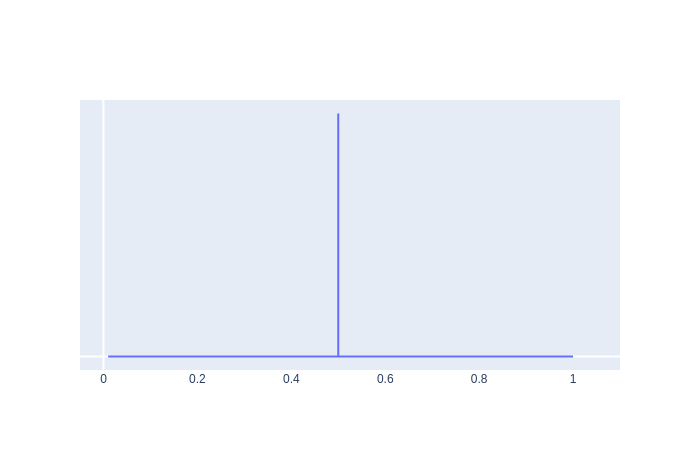
\includegraphics[width=\linewidth]{Dists/Bernoulli50.png}
		\caption{Modified Bernoulli distribution with $p=0$}
	\end{subfigure}%
	\begin{subfigure}{.5\textwidth}
		\centering
		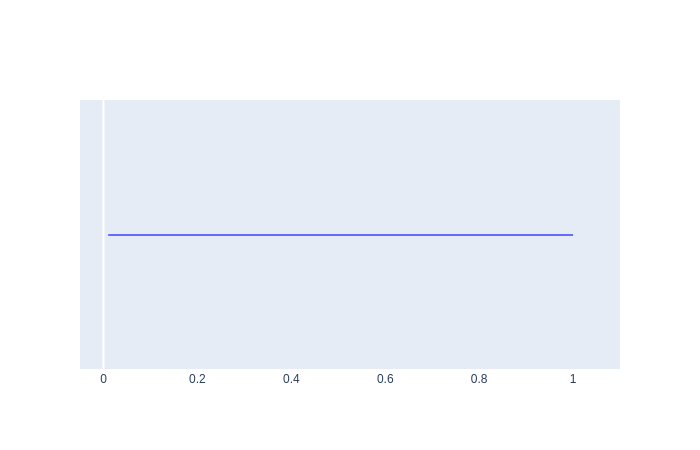
\includegraphics[width=\linewidth]{Dists/Beta50.png}
		\caption{Beta distribution with $\beta=1$ and $\alpha=1$}
	\end{subfigure}
	\caption{Edge guard size distribution for $\lambda = 0.5$}
	\label{fig:dist_lambda50}
\end{figure}%
\begin{figure}[H]
\centering
\begin{subfigure}{.5\textwidth}
	\centering
	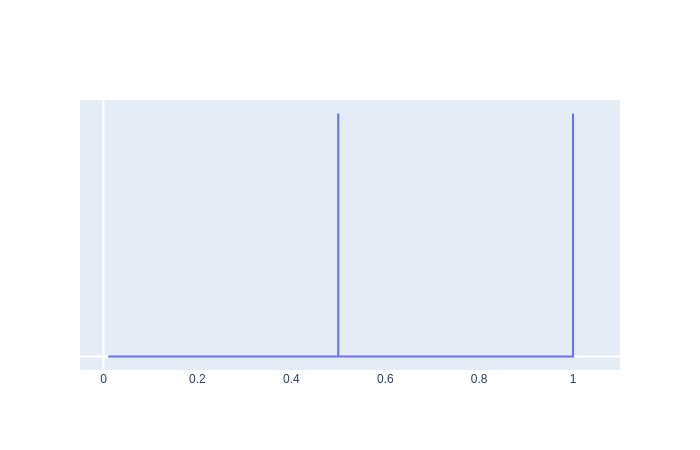
\includegraphics[width=\linewidth]{Dists/Bernoulli75.png}
	\caption{Modified Bernoulli distribution with $p=0.5$}
\end{subfigure}%
\begin{subfigure}{.5\textwidth}
	\centering
	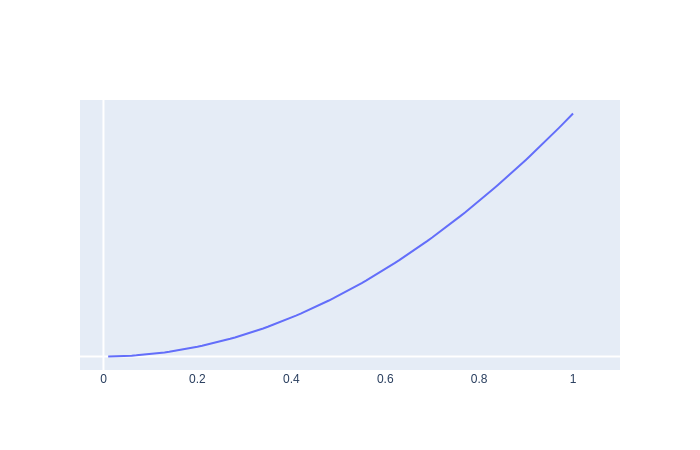
\includegraphics[width=\linewidth]{Dists/Beta75.png}
	\caption{Beta distribution with $\beta=1$ and $\alpha=3$}
\end{subfigure}
\caption{Edge guard size distribution for $\lambda = 0.75$}
\label{fig:dist_lambda75}
\end{figure}%
\begin{figure}[H]
\centering
\begin{subfigure}{.5\textwidth}
	\centering
	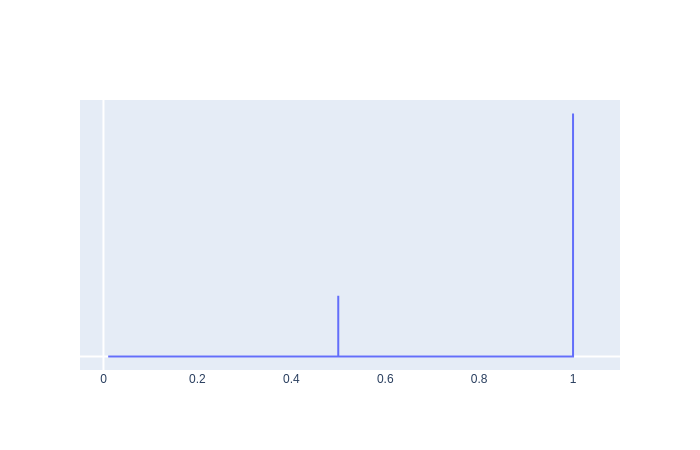
\includegraphics[width=\linewidth]{Dists/Bernoulli90.png}
	\caption{Modified Bernoulli distribution with $p=0.8$}
\end{subfigure}%
\begin{subfigure}{.5\textwidth}
	\centering
	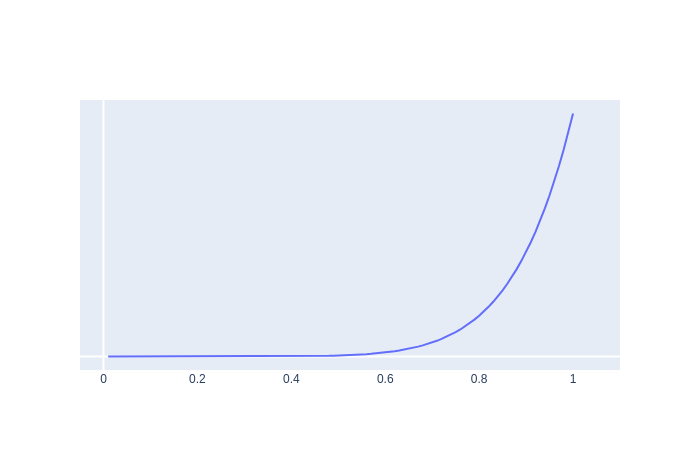
\includegraphics[width=\linewidth]{Dists/Beta90.png}
	\caption{Beta distribution with $\beta=1$ and $\alpha=9$}
\end{subfigure}
\caption{Edge guard size distribution for $\lambda = 0.9$}
\label{fig:dist_lambda90}
\end{figure}

Once we have determined the size for a configuration set we need to consider how the set is constructed. We can simply create a random set of configurations without any notion of features, we call this a \textit{configuration based} approach. Alternatively we can use a \textit{feature based} approach where we create sets by looking at features. Consider features $f_0, \dots, f_m$, we can create a boolean function that is the conjunction of $k$ features where every feature in the conjunction has probability $0.5$ of being negated.  For example when using $k=3$ and $m=5$ we might get boolean formula $f_1 \wedge \neg f_2 \wedge \neg f_4$. Such a boolean formula corresponds to a set of configurations of size $2^{m-k}$ and a relative size $\frac{2^{m-k}}{2^m} = 2^{-k}$, so when creating a set with relative size $r$ we choose $k = \min(m, \lfloor -\log_2{r} \rfloor)$. When using a feature based approach we can only create sets that have a relative size of $\frac{1}{2^i}$ for some $i \in \mathbb{N}$.

We can create 4 types of games:
\begin{enumerate}
	\item Bernoulli distributed and feature based. These games are most similar to the model verification games.
	\item Bernoulli distributed and configuration based. These games do have the characteristics of a model verification game in terms of set size but have unstructured sets guarding the edges. Furthermore with a configuration based approach less guard sets will be identical than with a feature based approach.
	\item Beta distributed and configuration based. These games are most different from the model verification games.
	\item Beta distributed and feature based. Games created in this way do not have the average relative set size of $\lambda$ because the feature based approach can only create sets of size $\frac{1}{2^i}$ for any $\lambda \geq \frac{1}{2}$ almost all the sets have either relative size $\frac{1}{2}$ or $1$, so  this creates almost the exact same games as using the Bernoulli distribution only with an incorrect average relative set size. Therefore we will not consider this category of games.
\end{enumerate}

We create four sets of random games. For random games of type 1,2 and 3 we create 25 games: game 75 to game 99, where game $i$ has $\lambda=\frac{i}{100}$ and a random number of features, nodes, edges and maximum priority. Furthermore we create 52 games to evaluate how the algorithm scales when the number of features becomes larger. For every $i \in [2,15]$ we create random games $i$a, $i$b, $i$c and $i$d of type 1 with $\lambda=0.92$, $i$ features and a random number of nodes, edges and maximum priority. 

Besides the number of configurations and the value for $\lambda$ we need to choose the number of vertices for a game, the minimum number of successors of a vertex, the maximum number of successors of a vertex and the number of distinct priorities in the game. The number of minimum and maximum successor is decides per game. So if we pick $l$ and $h$ as the number of minimum and maximum respectively then for every vertex of the game we uniformly pick its number of successors between $l$ and $h$.

Table \ref{tab_random_games} shows the different categories of games and the corresponding parameters. The minimum number of successors per vertex is always 1 so this value is omitted from the table.

\begin{table}[]
\centering
	\begin{tabular}{|l|l|l|l|l|l|l|}
		\hline
		Category & \# vertices & \shortstack{Maximum \\\# successors} & \shortstack{\# distinct\\priorities} & \# confs  & $\lambda$ \\ \hline
		Type 1, scale in $\lambda$ & $100-600$            & $3-20$                   & $1-10$                          & $2^{4}-2^{12}$ & $\frac{\textit{game nr}}{100}$            \\ \hline
		Type 2, scale in $\lambda$ & $100-600$            & $3-20$                   & $1-10$                          & $2^{4}-2^{12}$ & $\frac{\textit{game nr}}{100}$            \\ \hline
		Type 3, scale in $\lambda$ & $100-600$            & $3-20$                   & $1-10$                          & $2^{4}-2^{12}$ & $\frac{\textit{game nr}}{100}$            \\ \hline
		Type 1, scale in \# confs          & $100-600$            &  $3-20$                   & $1-10$                          & $2^\textit{game nr}$                & $0.92$                   \\ \hline
	\end{tabular}
\caption{Categories of random games}
	\label{tab_random_games}
\end{table}


\section{Results}
In this section the experimental results are presented. The following algorithms are used to solve the 6 categories of games:
\begin{enumerate}
	\item Zielonka's recursive algorithm, product based
	\item Fixed-point iteration, product based
	\item Fixed-point iteration, local product based
	\item Zielonka's recursive algorithm, family based with explicit configuration representation
	\item Zielonka's recursive algorithm, family based with symbolic configuration representation
	\item Incremental pre-solve algorithm
	\item Incremental pre-solve algorithm, local
\end{enumerate}

The results presented is the time it took to solve the games, parsing times and projection (for product based approaches) are excluded. So the product based results are the sum of the solve times of the projections, parsing and projecting are not included in the result.

The exact times can be found in appendix \ref{appendix:resultsexact}, in this section the results are visualized and presented to be easily interpreted. In some cases the results in a graph are normalized meaning that the running times are divided by the running times of the first algorithm in the graph. Specifically for the random games the running times vary a lot so normalizing is required to properly visualize the results. The times are presented on a logarithmic scale, games that were unable to be completed (due to memory) are marked with a grey bar.

All the experiments are ran on a Linux x64 operating system with an Intel i5-4570 processor and 8GB of ram.
\subsection{Zielonka's family based}
We compare the running times of the Zielonka's family based approaches with the Zielonka's product based approach. First we look at the model verification games.
\begin{figure}[H]
	\includegraphics[width=1\linewidth]{"results/minepump/Zlnk product based_Zlnk fam based - explicit_Zlnk fam based - symbolic_"}
	\caption{Running time of Zielonka's algorithms on the minepump problem}
	\label{fig:minepumpzlnks}
\end{figure}%
\begin{figure}[H]
	\includegraphics[width=1\linewidth]{"results/elevator/Zlnk product based_Zlnk fam based - explicit_Zlnk fam based - symbolic_"}
	\caption{Running time of Zielonka's algorithms on the elevator problem}
	\label{fig:elevatorzlnks}
\end{figure}%
We can see that the performance of the explicit variant varies a lot between games. The symbolic variant greatly outperforms the product based approach for every problem.

Next we inspect the random games, first we look at the games with a variable $\lambda$ and a random number of features. The graphs are normalized and the y-axis is cut off at 5.
\begin{figure}[H]
\includegraphics[width=1\linewidth]{"results/FF_randomgames/Zlnk product based_Zlnk fam based - explicit_Zlnk fam based - symbolic_"}
\caption{Running time of Zielonka's algorithms on randomgames of type 1 with $\lambda = \frac{\textit{game nr}}{100}$, times are normalized and the y-axis is cut off at 5}
\label{fig:elevatorzlnks}
\end{figure}%
\begin{figure}[H]
\includegraphics[width=1\linewidth]{"results/FC_randomgames/Zlnk product based_Zlnk fam based - explicit_Zlnk fam based - symbolic_"}
\caption{Running time of Zielonka's algorithms on randomgames of type 2 with $\lambda = \frac{\textit{game nr}}{100}$, times are normalized and the y-axis is cut off at 5}
\label{fig:elevatorzlnks}
\end{figure}%
\begin{figure}[H]
\includegraphics[width=1\linewidth]{"results/BC_randomgames/Zlnk product based_Zlnk fam based - explicit_Zlnk fam based - symbolic_"}
\caption{Running time of Zielonka's algorithms on randomgames of type 3 with $\lambda = \frac{\textit{game nr}}{100}$, times are normalized and the y-axis is cut off at 5}
\label{fig:elevatorzlnks}
\end{figure}%
For type 1 games we see that when $\lambda$ gets bigger the family based symbolic approach starts winning from the product based approach. There are a few exceptions to this, games 80, 82 and 86, all three of these games have only 4 features. As we will see later the less features there are in a game the worse the family based approaches perform.

For type 2 the explicit variant performs very similar to the type 1 games, however the symbolic approach performs much worse. This is due to the unstructured nature of the configuration sets which negatively influences bdd performance but has no effect on the explicit set operation. We also see the explicit algorithm outperforming the symbolic algorithm in some cases.

For type 3 games the product based approach performs generally better than the family based approaches unless $\lambda$ becomes very high.

Next we inspect how the algorithms scale in terms of number of features
\begin{figure}[H]
\includegraphics[width=1\linewidth]{"results/randomscalegames/Zlnk product based_Zlnk fam based - explicit_Zlnk fam based - symbolic_"}
\caption{Running time of Zielonka's algorithms on randomgames of type 1 with $\lambda = 0.92$ and the number of features equal to the $\textit{game nr}$, times are normalized and the y-axis is cut off at 5}
\label{fig:elevatorzlnks}
\end{figure}%
We can clearly conclude that as the number of features increases the family based symbolic approach performs better compared to the product based approach.

Overall we can conclude that the explicit algorithm performs somewhat arbitrary, however the symbolic algorithm performs really well for model checking problems and random games that have similar properties. Also we can conclude that the algorithms scales well in terms of number of features.


\subsection{Incremental pre-solve algorithm}
We compare the running times of the incremental pre-solve approaches with the fixed-point iteration product based algorithm. First we look at the model verification games.
\begin{figure}[H]
	\includegraphics[width=1\linewidth]{"results/minepump/Fixed-point product based_Incremental pre-solve_"}
	\caption{Running time of the incremental pre-solve algorithms on the minepump problem}
	\label{fig:minepumpzlnks}
\end{figure}%
\begin{figure}[H]
	\includegraphics[width=1\linewidth]{"results/elevator/Fixed-point product based_Incremental pre-solve_"}
	\caption{Running time of the incremental pre-solve algorithms on the elevator problem. Game 3, 4 and 5 were not able to be finished }
	\label{fig:elevatorzlnks}
\end{figure}%
The performance of the incremental pre-solve algorithm is generally worse that the product based approach, we do see however that the local variant is better in some cases.

Next we inspect the random games, first we look at the games with a variable $\lambda$ and a random number of features. The graphs are normalized and the y-axis is cut off at 5.
\begin{figure}[H]
	\includegraphics[width=1\linewidth]{"results/FF_randomgames/Fixed-point product based_Incremental pre-solve_"}
	\caption{Running time of the incremental pre-solve algorithms on randomgames of type 1 with $\lambda = \frac{\textit{game nr}}{100}$, times are normalized and the y-axis is cut off at 5}
	\label{fig:elevatorzlnks}
\end{figure}%
\begin{figure}[H]
	\includegraphics[width=1\linewidth]{"results/FC_randomgames/Fixed-point product based_Incremental pre-solve_"}
	\caption{Running time of incremental pre-solve algorithms on randomgames of type 2 with $\lambda = \frac{\textit{game nr}}{100}$, times are normalized and the y-axis is cut off at 5}
	\label{fig:elevatorzlnks}
\end{figure}%
\begin{figure}[H]
	\includegraphics[width=1\linewidth]{"results/BC_randomgames/Fixed-point product based_Incremental pre-solve_"}
	\caption{Running time of incremental pre-solve algorithms on randomgames of type 3 with $\lambda = \frac{\textit{game nr}}{100}$, times are normalized and the y-axis is cut off at 5}
	\label{fig:elevatorzlnks}
\end{figure}%
For type 1 games we see that when $\lambda$ gets bigger the family based approaches start performing better, specifically the local variant.

For type 2 the family based local approach still performs quite well when $\lambda$ gets bigger. For type 3 games the product based approach outperforms the family based approaches.

Next we inspect how the algorithms scales in terms of number of features
\begin{figure}[H]
	\includegraphics[width=1\linewidth]{"results/randomscalegames/Fixed-point product based_Incremental pre-solve_"}
	\caption{Running time of incremental pre-solve algorithms on randomgames of type 1 with $\lambda = 0.92$ and the number of features equal to the $\textit{game nr}$, times are normalized and the y-axis is cut off at 5}
	\label{fig:elevatorzlnks}
\end{figure}%
The number of features seems to have little effect on the performance of the family based approaches.

Overall we can see that the local variant performs significantly better, specifically for random games. The local approach seems to be hit or miss where in some cases it finds vertex $0$ quickly without traversing the tree but in other cases it has little effect compared to the global variant. Model verification problems generally have a vertex $0$ that depends on a large part of the game and are therefore not very suitable to be solved locally. (TODO cite oid)

\subsection{Incremental pre-solve local algorithm}
We compare the running times of the incremental pre-solve approaches with the fixed-point iteration product based algorithm. First we look at the model verification games.
\begin{figure}[H]
	\includegraphics[width=1\linewidth]{"results/minepump/Fixed-point local product based_Incremental pre-solve local_"}
	\caption{Running time of the incremental pre-solve local algorithms on the minepump problem}
	\label{fig:minepumpzlnks}
\end{figure}%
\begin{figure}[H]
	\includegraphics[width=1\linewidth]{"results/elevator/Fixed-point local product based_Incremental pre-solve local_"}
	\caption{Running time of the incremental pre-solve local algorithms on the elevator problem}
	\label{fig:elevatorzlnks}
\end{figure}%
The performance of the incremental pre-solve algorithm is generally worse that the product based approach, we do see however that the local variant is better in some cases.

Next we inspect the random games, first we look at the games with a variable $\lambda$ and a random number of features. The graphs are normalized and the y-axis is cut off at 5.
\begin{figure}[H]
	\includegraphics[width=1\linewidth]{"results/FF_randomgames/Fixed-point local product based_Incremental pre-solve local_"}
	\caption{Running time of the incremental pre-solve local algorithms on randomgames of type 1 with $\lambda = \frac{\textit{game nr}}{100}$, times are normalized and the y-axis is cut off at 5}
	\label{fig:elevatorzlnks}
\end{figure}%
\begin{figure}[H]
	\includegraphics[width=1\linewidth]{"results/FC_randomgames/Fixed-point local product based_Incremental pre-solve local_"}
	\caption{Running time of incremental pre-solve local algorithms on randomgames of type 2 with $\lambda = \frac{\textit{game nr}}{100}$, times are normalized and the y-axis is cut off at 5}
	\label{fig:elevatorzlnks}
\end{figure}%
\begin{figure}[H]
	\includegraphics[width=1\linewidth]{"results/BC_randomgames/Fixed-point local product based_Incremental pre-solve local_"}
	\caption{Running time of incremental pre-solve local algorithms on randomgames of type 3 with $\lambda = \frac{\textit{game nr}}{100}$, times are normalized and the y-axis is cut off at 5}
	\label{fig:elevatorzlnks}
\end{figure}%
For type 1 games we see that when $\lambda$ gets bigger the family based approaches start performing better, specifically the local variant.

For type 2 the family based local approach still performs quite well when $\lambda$ gets bigger. For type 3 games the product based approach outperforms the family based approaches.

Next we inspect how the algorithms scales in terms of number of features
\begin{figure}[H]
	\includegraphics[width=1\linewidth]{"results/randomscalegames/Fixed-point local product based_Incremental pre-solve local_"}
	\caption{Running time of incremental pre-solve local algorithms on randomgames of type 1 with $\lambda = 0.92$ and the number of features equal to the $\textit{game nr}$, times are normalized and the y-axis is cut off at 5}
	\label{fig:elevatorzlnks}
\end{figure}%
The number of features seems to have little effect on the performance of the family based approaches.

Overall we can see that the local variant performs significantly better, specifically for random games. The local approach seems to be hit or miss where in some cases it finds vertex $0$ quickly without traversing the tree but in other cases it has little effect compared to the global variant. Model verification problems generally have a vertex $0$ that depends on a large part of the game and are therefore not very suitable to be solved locally. (TODO cite oid)

\subsection{Comparison}
After comparing family based and product based variants of the same algorithm we compare the algorithms overall. We do so by comparing the average solve time of the for every set of games.

First we compare the product based algorithms:\\
\begin{tabular}{|l|l|l|l|}
	\hline
	& \shortstack{Zlnk product based\\\ } & \shortstack{Fixed-point product based\\global} & \shortstack{Fixed-point product based\\local} \\ \hline
	minepump& 118 ms& 4719 ms& 4469 ms\\ \hline
	elevator& 36540 ms& 9842835 ms& 1713073 ms\\ \hline
	FF randomgames& 55 ms& 413 ms& 324 ms\\ \hline
	FC randomgames& 54 ms& 413 ms& 381 ms\\ \hline
	BC randomgames& 55 ms& 416 ms& 351 ms\\ \hline
	randomscalegames& 108 ms& 408 ms& 381 ms\\ \hline
\end{tabular}

Next we compare the family based algorithms:\\
\begin{tabular}{|l|l|l|l|l|}
	\hline
	& \shortstack{Zlnk fam based\\ explicit} & \shortstack{Zlnk fam based\\symbolic} & \shortstack{Incremental pre-solve\\global} & \shortstack{Incremental pre-solve\\local} \\ \hline
	minepump& 391 ms& 16 ms& 1154 ms& 672 ms\\ \hline
	elevator& 46775 ms& 6592 ms& 299246 ms& 381041 ms\\ \hline
	FF randomgames& 513 ms& 59 ms& 274 ms& 40 ms\\ \hline
	FC randomgames& 1149 ms& 2569 ms& 8283 ms& 1507 ms\\ \hline
	BC randomgames& 1117 ms& 2114 ms& 12733 ms& 4365 ms\\ \hline
	randomscalegames& 397 ms& 9 ms& 205 ms& 24 ms\\ \hline
\end{tabular}

\pagebreak
\begin{appendices}
\section{Auxiliary theorems and lemma's}
\label{appendix:proves}
\begin{lemma}
	\label{lem_md_ineq}
	For $d,m \in \mathbb{N}$ with $d>1$ and $m \geq 0$ the following inequality holds:
	\[ (m+d-1)^d + m+1 \leq (m+d)^d \]
	\begin{proof}
		We expand the inequality.
		\begin{align*}
		(m+d-1)^d + m + 1 & \leq (m+d)^d\\
		(m+d-1)(m+d-1)^{d-1} + m + 1 & \leq (m+d)(m+d)^{d-1}\\
		m(m+d-1)^{d-1} + d(m+d-1)^{d-1} - (m+d-1)^{d-1} + m + 1 & \leq m(m+d)^{d-1} + d(m+d)^{d-1}
		\end{align*}
		Since $d > 1$ and $m \geq 0$ we can see that the left hand term $m(m+d-1)^{d-1}$ is less or equal to the right hand term $m(m+d)^{d-1}$, similarly the left hand term $d(m+d-1)^{d-1}$ is less or equal to the right hand term $d(m+d)^{d-1}$. Finally the term $(m+d-1)^{d-1} \geq (m+1)^{d-1} \geq m+1$ and therefore $- (m+d-1)^{d-1} + m + 1  \leq 0$. This proves the lemma.
	\end{proof}
\end{lemma}
\section{Running time results}
\label{appendix:resultsexact}
\subsection{minepump}
\begin{tabular}{|l|l|}
	\hline
	& Zlnk product based \\ \hline
	Game 1 & 145.710686 ms \\ \hline
	Game 2 & 171.767544 ms \\ \hline
	Game 3 & 589.163537 ms \\ \hline
	Game 4 & 620.295945 ms \\ \hline
	Game 5 & 533.288498 ms \\ \hline
	Game 6 & 777.771697 ms \\ \hline
	Game 7 & 465.356122 ms \\ \hline
	Game 8 & 139.804051 ms \\ \hline
	Game 9 & 411.34498 ms \\ \hline
\end{tabular}
\begin{tabular}{|l|l|}
	\hline
	& Fixed-point product based \\ \hline
	Game 1 & 130.587291 ms \\ \hline
	Game 2 & 135.382598 ms \\ \hline
	Game 3 & 460.184224 ms \\ \hline
	Game 4 & 37898.67001 ms \\ \hline
	Game 5 & 1346.308334 ms \\ \hline
	Game 6 & 928.083238 ms \\ \hline
	Game 7 & 669.829938 ms \\ \hline
	Game 8 & 80.328725 ms \\ \hline
	Game 9 & 823.229266 ms \\ \hline
\end{tabular}
\begin{tabular}{|l|l|}
	\hline
	& Fixed-point local product based \\ \hline
	Game 1 & 66.477775 ms \\ \hline
	Game 2 & 82.189287 ms \\ \hline
	Game 3 & 278.245894 ms \\ \hline
	Game 4 & 37764.888965 ms \\ \hline
	Game 5 & 833.712816 ms \\ \hline
	Game 6 & 544.744721 ms \\ \hline
	Game 7 & 562.618467 ms \\ \hline
	Game 8 & 8.503434 ms \\ \hline
	Game 9 & 75.415805 ms \\ \hline
\end{tabular}
\begin{tabular}{|l|l|}
	\hline
	& Zlnk fam based - explicit \\ \hline
	Game 1 & 87.111158 ms \\ \hline
	Game 2 & 158.648592 ms \\ \hline
	Game 3 & 632.834564 ms \\ \hline
	Game 4 & 905.322212 ms \\ \hline
	Game 5 & 285.163541 ms \\ \hline
	Game 6 & 1031.566116 ms \\ \hline
	Game 7 & 326.632454 ms \\ \hline
	Game 8 & 25.146327 ms \\ \hline
	Game 9 & 166.074354 ms \\ \hline
\end{tabular}
\begin{tabular}{|l|l|}
	\hline
	& Zlnk fam based - symbolic \\ \hline
	Game 1 & 5.052944 ms \\ \hline
	Game 2 & 8.372276 ms \\ \hline
	Game 3 & 32.35237 ms \\ \hline
	Game 4 & 45.629408 ms \\ \hline
	Game 5 & 16.072678 ms \\ \hline
	Game 6 & 54.307865 ms \\ \hline
	Game 7 & 15.43434 ms \\ \hline
	Game 8 & 2.104151 ms \\ \hline
	Game 9 & 9.604102 ms \\ \hline
\end{tabular}
\begin{tabular}{|l|l|}
	\hline
	& Incremental pre-solve \\ \hline
	Game 1 & 402.898316 ms \\ \hline
	Game 2 & 341.198461 ms \\ \hline
	Game 3 & 1255.949764 ms \\ \hline
	Game 4 & 4803.836362 ms \\ \hline
	Game 5 & 1092.277622 ms \\ \hline
	Game 6 & 831.198424 ms \\ \hline
	Game 7 & 917.083359 ms \\ \hline
	Game 8 & 1.761178 ms \\ \hline
	Game 9 & 742.183235 ms \\ \hline
\end{tabular}
\begin{tabular}{|l|l|}
	\hline
	& Incremental pre-solve local \\ \hline
	Game 1 & 402.728056 ms \\ \hline
	Game 2 & 1.827667 ms \\ \hline
	Game 3 & 184.726048 ms \\ \hline
	Game 4 & 3480.033761 ms \\ \hline
	Game 5 & 583.474132 ms \\ \hline
	Game 6 & 473.593019 ms \\ \hline
	Game 7 & 914.134888 ms \\ \hline
	Game 8 & 1.174847 ms \\ \hline
	Game 9 & 4.019017 ms \\ \hline
\end{tabular}
\subsection{elevator}
\begin{tabular}{|l|l|}
	\hline
	& Zlnk product based \\ \hline
	Game 1 & 269357.17363 ms \\ \hline
	Game 2 & 429856.472992 ms \\ \hline
	Game 3a & 718657.056545 ms \\ \hline
	Game 3b & 716411.123774 ms \\ \hline
	Game 5 & 212494.552309 ms \\ \hline
	Game 6 & 0.260769 ms \\ \hline
	Game 7 & 0.260798 ms \\ \hline
\end{tabular}
\begin{tabular}{|l|l|}
	\hline
	& Fixed-point product based \\ \hline
	Game 1 & 880895.014563 ms \\ \hline
	Game 2 & 8790000.10349 ms \\ \hline
	Game 3a & 29387446.6626 ms \\ \hline
	Game 3b & 29423372.371 ms \\ \hline
	Game 5 & 418128.687347 ms \\ \hline
	Game 6 & 0.182554 ms \\ \hline
	Game 7 & 0.182125 ms \\ \hline
\end{tabular}
\begin{tabular}{|l|l|}
	\hline
	& Fixed-point local product based \\ \hline
	Game 1 & 423068.957211 ms \\ \hline
	Game 2 & 1983814.2006 ms \\ \hline
	Game 3a & 4635988.08945 ms \\ \hline
	Game 3b & 4666038.77282 ms \\ \hline
	Game 5 & 282602.487182 ms \\ \hline
	Game 6 & 0.11491 ms \\ \hline
	Game 7 & 0.111502 ms \\ \hline
\end{tabular}
\begin{tabular}{|l|l|}
	\hline
	& Zlnk fam based - explicit \\ \hline
	Game 1 & 33879.405405 ms \\ \hline
	Game 2 & 51596.003539 ms \\ \hline
	Game 3a & \dag \\ \hline
	Game 3b & \dag \\ \hline
	Game 5 & 37210.889792 ms \\ \hline
	Game 6 & 0.099443 ms \\ \hline
	Game 7 & 0.120632 ms \\ \hline
\end{tabular}
\begin{tabular}{|l|l|}
	\hline
	& Zlnk fam based - symbolic \\ \hline
	Game 1 & 14964.371693 ms \\ \hline
	Game 2 & 21803.007101 ms \\ \hline
	Game 3a & 38288.893506 ms \\ \hline
	Game 3b & 38213.782824 ms \\ \hline
	Game 5 & 16324.397915 ms \\ \hline
	Game 6 & 0.012454 ms \\ \hline
	Game 7 & 0.012368 ms \\ \hline
\end{tabular}
\begin{tabular}{|l|l|}
	\hline
	& Incremental pre-solve \\ \hline
	Game 1 & 236171.44533 ms \\ \hline
	Game 2 & 960813.557869 ms \\ \hline
	Game 3a & \dag \\ \hline
	Game 3b & \dag \\ \hline
	Game 5 & \dag \\ \hline
	Game 6 & 0.011157 ms \\ \hline
	Game 7 & 0.0103 ms \\ \hline
\end{tabular}
\begin{tabular}{|l|l|}
	\hline
	& Incremental pre-solve local \\ \hline
	Game 1 & 29941.840644 ms \\ \hline
	Game 2 & 317217.608246 ms \\ \hline
	Game 3a & 1133904.4743 ms \\ \hline
	Game 3b & 1152374.57835 ms \\ \hline
	Game 5 & 33845.973375 ms \\ \hline
	Game 6 & 0.010736 ms \\ \hline
	Game 7 & 0.010461 ms \\ \hline
\end{tabular}
\subsection{FF randomgames}
\begin{tabular}{|l|l|}
	\hline
	& Zlnk product based \\ \hline
	Game 50 & 22.894099 ms \\ \hline
	Game 51 & 415.090564 ms \\ \hline
	Game 52 & 3.531167 ms \\ \hline
	Game 53 & 2.861018 ms \\ \hline
	Game 54 & 94.868137 ms \\ \hline
	Game 55 & 6.835354 ms \\ \hline
	Game 56 & 469.55704 ms \\ \hline
	Game 57 & 19.217615 ms \\ \hline
	Game 58 & 5.671594 ms \\ \hline
	Game 59 & 21.520462 ms \\ \hline
	Game 60 & 82.895336 ms \\ \hline
	Game 61 & 6.332443 ms \\ \hline
	Game 62 & 85.507286 ms \\ \hline
	Game 63 & 46.017808 ms \\ \hline
	Game 64 & 15.773509 ms \\ \hline
	Game 65 & 370.805409 ms \\ \hline
	Game 66 & 22.776748 ms \\ \hline
	Game 67 & 7.120147 ms \\ \hline
	Game 68 & 81.248511 ms \\ \hline
	Game 69 & 38.474281 ms \\ \hline
	Game 70 & 2.863258 ms \\ \hline
	Game 71 & 62.639661 ms \\ \hline
	Game 72 & 0.843288 ms \\ \hline
	Game 73 & 5.831069 ms \\ \hline
	Game 74 & 48.460654 ms \\ \hline
	Game 75 & 147.861501 ms \\ \hline
	Game 76 & 461.039 ms \\ \hline
	Game 77 & 96.339976 ms \\ \hline
	Game 78 & 383.656332 ms \\ \hline
	Game 79 & 755.153118 ms \\ \hline
	Game 80 & 2.733223 ms \\ \hline
	Game 81 & 185.213669 ms \\ \hline
	Game 82 & 1.475768 ms \\ \hline
	Game 83 & 22.639925 ms \\ \hline
	Game 84 & 193.419532 ms \\ \hline
	Game 85 & 14.283935 ms \\ \hline
	Game 86 & 6.635476 ms \\ \hline
	Game 87 & 17.298111 ms \\ \hline
	Game 88 & 7.915332 ms \\ \hline
	Game 89 & 246.627127 ms \\ \hline
	Game 90 & 631.734621 ms \\ \hline
	Game 91 & 123.777906 ms \\ \hline
	Game 92 & 465.960801 ms \\ \hline
	Game 93 & 117.739068 ms \\ \hline
	Game 94 & 98.094232 ms \\ \hline
	Game 95 & 227.341992 ms \\ \hline
	Game 96 & 379.466667 ms \\ \hline
	Game 97 & 131.677711 ms \\ \hline
	Game 98 & 35.736698 ms \\ \hline
	Game 99 & 1.010203 ms \\ \hline
\end{tabular}
\begin{tabular}{|l|l|}
	\hline
	& Fixed-point product based \\ \hline
	Game 50 & 20.566329 ms \\ \hline
	Game 51 & 6744.284861 ms \\ \hline
	Game 52 & 1.47327 ms \\ \hline
	Game 53 & 4.295792 ms \\ \hline
	Game 54 & 29.14741 ms \\ \hline
	Game 55 & 14.425234 ms \\ \hline
	Game 56 & 912.128577 ms \\ \hline
	Game 57 & 199.442715 ms \\ \hline
	Game 58 & 6.650932 ms \\ \hline
	Game 59 & 30.331524 ms \\ \hline
	Game 60 & 266.762206 ms \\ \hline
	Game 61 & 2.756214 ms \\ \hline
	Game 62 & 215.868882 ms \\ \hline
	Game 63 & 226.614402 ms \\ \hline
	Game 64 & 83.090986 ms \\ \hline
	Game 65 & 266.050094 ms \\ \hline
	Game 66 & 121.173001 ms \\ \hline
	Game 67 & 30.477553 ms \\ \hline
	Game 68 & 43.78565 ms \\ \hline
	Game 69 & 28.032054 ms \\ \hline
	Game 70 & 0.396067 ms \\ \hline
	Game 71 & 28.951018 ms \\ \hline
	Game 72 & 0.200488 ms \\ \hline
	Game 73 & 10.418019 ms \\ \hline
	Game 74 & 143.527764 ms \\ \hline
	Game 75 & 46.377756 ms \\ \hline
	Game 76 & 173.248219 ms \\ \hline
	Game 77 & 1023.572304 ms \\ \hline
	Game 78 & 1500.871069 ms \\ \hline
	Game 79 & 473.520308 ms \\ \hline
	Game 80 & 1.31479 ms \\ \hline
	Game 81 & 1054.141901 ms \\ \hline
	Game 82 & 1.317754 ms \\ \hline
	Game 83 & 24.022014 ms \\ \hline
	Game 84 & 947.266091 ms \\ \hline
	Game 85 & 9.411088 ms \\ \hline
	Game 86 & 17.27655 ms \\ \hline
	Game 87 & 5.299216 ms \\ \hline
	Game 88 & 5.561753 ms \\ \hline
	Game 89 & 1103.733905 ms \\ \hline
	Game 90 & 642.737385 ms \\ \hline
	Game 91 & 210.113964 ms \\ \hline
	Game 92 & 140.735555 ms \\ \hline
	Game 93 & 124.311004 ms \\ \hline
	Game 94 & 465.467471 ms \\ \hline
	Game 95 & 1940.174842 ms \\ \hline
	Game 96 & 1066.142203 ms \\ \hline
	Game 97 & 202.031576 ms \\ \hline
	Game 98 & 24.381076 ms \\ \hline
	Game 99 & 0.153665 ms \\ \hline
\end{tabular}
\begin{tabular}{|l|l|}
	\hline
	& Fixed-point local product based \\ \hline
	Game 50 & 20.595845 ms \\ \hline
	Game 51 & 6292.631423 ms \\ \hline
	Game 52 & 1.398527 ms \\ \hline
	Game 53 & 4.302088 ms \\ \hline
	Game 54 & 29.24289 ms \\ \hline
	Game 55 & 7.193027 ms \\ \hline
	Game 56 & 472.727188 ms \\ \hline
	Game 57 & 169.646163 ms \\ \hline
	Game 58 & 6.664684 ms \\ \hline
	Game 59 & 10.358405 ms \\ \hline
	Game 60 & 267.307192 ms \\ \hline
	Game 61 & 1.508336 ms \\ \hline
	Game 62 & 205.976637 ms \\ \hline
	Game 63 & 130.156094 ms \\ \hline
	Game 64 & 29.198676 ms \\ \hline
	Game 65 & 197.182221 ms \\ \hline
	Game 66 & 120.811351 ms \\ \hline
	Game 67 & 20.417376 ms \\ \hline
	Game 68 & 18.646781 ms \\ \hline
	Game 69 & 28.136298 ms \\ \hline
	Game 70 & 0.381035 ms \\ \hline
	Game 71 & 27.067918 ms \\ \hline
	Game 72 & 0.204019 ms \\ \hline
	Game 73 & 3.462291 ms \\ \hline
	Game 74 & 143.903704 ms \\ \hline
	Game 75 & 36.805055 ms \\ \hline
	Game 76 & 167.128798 ms \\ \hline
	Game 77 & 383.250688 ms \\ \hline
	Game 78 & 564.751313 ms \\ \hline
	Game 79 & 473.792807 ms \\ \hline
	Game 80 & 1.086947 ms \\ \hline
	Game 81 & 1053.657412 ms \\ \hline
	Game 82 & 1.324338 ms \\ \hline
	Game 83 & 14.837088 ms \\ \hline
	Game 84 & 357.204857 ms \\ \hline
	Game 85 & 9.476771 ms \\ \hline
	Game 86 & 7.262061 ms \\ \hline
	Game 87 & 5.352538 ms \\ \hline
	Game 88 & 2.610671 ms \\ \hline
	Game 89 & 543.43552 ms \\ \hline
	Game 90 & 367.617943 ms \\ \hline
	Game 91 & 87.154413 ms \\ \hline
	Game 92 & 142.924215 ms \\ \hline
	Game 93 & 74.032315 ms \\ \hline
	Game 94 & 465.642971 ms \\ \hline
	Game 95 & 1939.324955 ms \\ \hline
	Game 96 & 1068.923695 ms \\ \hline
	Game 97 & 202.097029 ms \\ \hline
	Game 98 & 24.263109 ms \\ \hline
	Game 99 & 0.154271 ms \\ \hline
\end{tabular}
\begin{tabular}{|l|l|}
	\hline
	& Zlnk fam based - explicit \\ \hline
	Game 50 & 132.471665 ms \\ \hline
	Game 51 & 9419.058069 ms \\ \hline
	Game 52 & 2.7618 ms \\ \hline
	Game 53 & 17.544563 ms \\ \hline
	Game 54 & 581.81683 ms \\ \hline
	Game 55 & 71.685999 ms \\ \hline
	Game 56 & 2661.310318 ms \\ \hline
	Game 57 & 77.107864 ms \\ \hline
	Game 58 & 41.351346 ms \\ \hline
	Game 59 & 47.101189 ms \\ \hline
	Game 60 & 79.691535 ms \\ \hline
	Game 61 & 43.512465 ms \\ \hline
	Game 62 & 268.348187 ms \\ \hline
	Game 63 & 439.554763 ms \\ \hline
	Game 64 & 23.015237 ms \\ \hline
	Game 65 & 2598.745644 ms \\ \hline
	Game 66 & 26.532439 ms \\ \hline
	Game 67 & 48.409873 ms \\ \hline
	Game 68 & 150.920555 ms \\ \hline
	Game 69 & 41.092679 ms \\ \hline
	Game 70 & 0.704051 ms \\ \hline
	Game 71 & 65.254112 ms \\ \hline
	Game 72 & 0.367596 ms \\ \hline
	Game 73 & 9.710427 ms \\ \hline
	Game 74 & 28.357716 ms \\ \hline
	Game 75 & 6.084672 ms \\ \hline
	Game 76 & 2299.390861 ms \\ \hline
	Game 77 & 142.898393 ms \\ \hline
	Game 78 & 1406.919686 ms \\ \hline
	Game 79 & 858.03388 ms \\ \hline
	Game 80 & 5.400674 ms \\ \hline
	Game 81 & 270.81002 ms \\ \hline
	Game 82 & 2.407317 ms \\ \hline
	Game 83 & 65.527967 ms \\ \hline
	Game 84 & 363.863434 ms \\ \hline
	Game 85 & 2.711993 ms \\ \hline
	Game 86 & 19.38862 ms \\ \hline
	Game 87 & 5.777005 ms \\ \hline
	Game 88 & 2.419001 ms \\ \hline
	Game 89 & 255.358705 ms \\ \hline
	Game 90 & 1938.833122 ms \\ \hline
	Game 91 & 27.914326 ms \\ \hline
	Game 92 & 257.34058 ms \\ \hline
	Game 93 & 99.616438 ms \\ \hline
	Game 94 & 250.807913 ms \\ \hline
	Game 95 & 43.182079 ms \\ \hline
	Game 96 & 399.435036 ms \\ \hline
	Game 97 & 63.44707 ms \\ \hline
	Game 98 & 36.997553 ms \\ \hline
	Game 99 & 0.147938 ms \\ \hline
\end{tabular}
\begin{tabular}{|l|l|}
	\hline
	& Zlnk fam based - symbolic \\ \hline
	Game 50 & 30.411701 ms \\ \hline
	Game 51 & 2079.058824 ms \\ \hline
	Game 52 & 1.899092 ms \\ \hline
	Game 53 & 8.634299 ms \\ \hline
	Game 54 & 39.92786 ms \\ \hline
	Game 55 & 51.745846 ms \\ \hline
	Game 56 & 78.389071 ms \\ \hline
	Game 57 & 31.689397 ms \\ \hline
	Game 58 & 32.055879 ms \\ \hline
	Game 59 & 14.083391 ms \\ \hline
	Game 60 & 5.963575 ms \\ \hline
	Game 61 & 29.680534 ms \\ \hline
	Game 62 & 29.427663 ms \\ \hline
	Game 63 & 127.371121 ms \\ \hline
	Game 64 & 6.433852 ms \\ \hline
	Game 65 & 118.75719 ms \\ \hline
	Game 66 & 10.763784 ms \\ \hline
	Game 67 & 32.088827 ms \\ \hline
	Game 68 & 8.20797 ms \\ \hline
	Game 69 & 5.009418 ms \\ \hline
	Game 70 & 0.259005 ms \\ \hline
	Game 71 & 9.179291 ms \\ \hline
	Game 72 & 0.184988 ms \\ \hline
	Game 73 & 4.683395 ms \\ \hline
	Game 74 & 2.693721 ms \\ \hline
	Game 75 & 0.266035 ms \\ \hline
	Game 76 & 50.078993 ms \\ \hline
	Game 77 & 12.918694 ms \\ \hline
	Game 78 & 61.057056 ms \\ \hline
	Game 79 & 9.95944 ms \\ \hline
	Game 80 & 3.61149 ms \\ \hline
	Game 81 & 12.008958 ms \\ \hline
	Game 82 & 1.714712 ms \\ \hline
	Game 83 & 17.773642 ms \\ \hline
	Game 84 & 15.673699 ms \\ \hline
	Game 85 & 0.463345 ms \\ \hline
	Game 86 & 11.490767 ms \\ \hline
	Game 87 & 0.748539 ms \\ \hline
	Game 88 & 0.770723 ms \\ \hline
	Game 89 & 10.615619 ms \\ \hline
	Game 90 & 39.17593 ms \\ \hline
	Game 91 & 1.540775 ms \\ \hline
	Game 92 & 2.786512 ms \\ \hline
	Game 93 & 3.99316 ms \\ \hline
	Game 94 & 36.186725 ms \\ \hline
	Game 95 & 1.118923 ms \\ \hline
	Game 96 & 7.881691 ms \\ \hline
	Game 97 & 1.340903 ms \\ \hline
	Game 98 & 5.233279 ms \\ \hline
	Game 99 & 0.047058 ms \\ \hline
\end{tabular}
\begin{tabular}{|l|l|}
	\hline
	& Incremental pre-solve \\ \hline
	Game 50 & 46.080898 ms \\ \hline
	Game 51 & 2992.042268 ms \\ \hline
	Game 52 & 3.151228 ms \\ \hline
	Game 53 & 9.583558 ms \\ \hline
	Game 54 & 325.711561 ms \\ \hline
	Game 55 & 33.458447 ms \\ \hline
	Game 56 & 1539.005235 ms \\ \hline
	Game 57 & 143.532033 ms \\ \hline
	Game 58 & 21.824657 ms \\ \hline
	Game 59 & 54.624111 ms \\ \hline
	Game 60 & 122.370786 ms \\ \hline
	Game 61 & 23.554931 ms \\ \hline
	Game 62 & 109.501093 ms \\ \hline
	Game 63 & 203.673008 ms \\ \hline
	Game 64 & 35.808988 ms \\ \hline
	Game 65 & 1165.840461 ms \\ \hline
	Game 66 & 71.074647 ms \\ \hline
	Game 67 & 27.291058 ms \\ \hline
	Game 68 & 212.068661 ms \\ \hline
	Game 69 & 80.825415 ms \\ \hline
	Game 70 & 3.859968 ms \\ \hline
	Game 71 & 114.442028 ms \\ \hline
	Game 72 & 0.649724 ms \\ \hline
	Game 73 & 18.543163 ms \\ \hline
	Game 74 & 55.220584 ms \\ \hline
	Game 75 & 48.855116 ms \\ \hline
	Game 76 & 1419.192729 ms \\ \hline
	Game 77 & 253.275833 ms \\ \hline
	Game 78 & 1142.785118 ms \\ \hline
	Game 79 & 1962.348341 ms \\ \hline
	Game 80 & 6.247378 ms \\ \hline
	Game 81 & 524.071394 ms \\ \hline
	Game 82 & 2.152315 ms \\ \hline
	Game 83 & 71.00827 ms \\ \hline
	Game 84 & 206.907479 ms \\ \hline
	Game 85 & 20.351748 ms \\ \hline
	Game 86 & 18.925971 ms \\ \hline
	Game 87 & 26.118424 ms \\ \hline
	Game 88 & 8.694553 ms \\ \hline
	Game 89 & 143.203366 ms \\ \hline
	Game 90 & 192.609233 ms \\ \hline
	Game 91 & 143.36905 ms \\ \hline
	Game 92 & 11.604601 ms \\ \hline
	Game 93 & 0.505494 ms \\ \hline
	Game 94 & 4.989098 ms \\ \hline
	Game 95 & 2.18487 ms \\ \hline
	Game 96 & 1.447915 ms \\ \hline
	Game 97 & 1.369827 ms \\ \hline
	Game 98 & 86.552119 ms \\ \hline
	Game 99 & 0.02177 ms \\ \hline
\end{tabular}
\begin{tabular}{|l|l|}
	\hline
	& Incremental pre-solve local \\ \hline
	Game 50 & 9.018887 ms \\ \hline
	Game 51 & 1523.362457 ms \\ \hline
	Game 52 & 2.56276 ms \\ \hline
	Game 53 & 6.587165 ms \\ \hline
	Game 54 & 14.87686 ms \\ \hline
	Game 55 & 9.903866 ms \\ \hline
	Game 56 & 4.660675 ms \\ \hline
	Game 57 & 96.08021 ms \\ \hline
	Game 58 & 8.569419 ms \\ \hline
	Game 59 & 0.534212 ms \\ \hline
	Game 60 & 52.722595 ms \\ \hline
	Game 61 & 1.132779 ms \\ \hline
	Game 62 & 88.117407 ms \\ \hline
	Game 63 & 8.078743 ms \\ \hline
	Game 64 & 1.370403 ms \\ \hline
	Game 65 & 2.78775 ms \\ \hline
	Game 66 & 57.445895 ms \\ \hline
	Game 67 & 3.053301 ms \\ \hline
	Game 68 & 0.384612 ms \\ \hline
	Game 69 & 0.376439 ms \\ \hline
	Game 70 & 3.533979 ms \\ \hline
	Game 71 & 25.211715 ms \\ \hline
	Game 72 & 0.076533 ms \\ \hline
	Game 73 & 7.696058 ms \\ \hline
	Game 74 & 0.464487 ms \\ \hline
	Game 75 & 15.709783 ms \\ \hline
	Game 76 & 1.285309 ms \\ \hline
	Game 77 & 5.801185 ms \\ \hline
	Game 78 & 6.765665 ms \\ \hline
	Game 79 & 0.722754 ms \\ \hline
	Game 80 & 0.953798 ms \\ \hline
	Game 81 & 3.425409 ms \\ \hline
	Game 82 & 0.217681 ms \\ \hline
	Game 83 & 1.021352 ms \\ \hline
	Game 84 & 2.749428 ms \\ \hline
	Game 85 & 0.121502 ms \\ \hline
	Game 86 & 1.616307 ms \\ \hline
	Game 87 & 0.078561 ms \\ \hline
	Game 88 & 0.224175 ms \\ \hline
	Game 89 & 2.50544 ms \\ \hline
	Game 90 & 1.621967 ms \\ \hline
	Game 91 & 0.683825 ms \\ \hline
	Game 92 & 0.294685 ms \\ \hline
	Game 93 & 0.503414 ms \\ \hline
	Game 94 & 4.977672 ms \\ \hline
	Game 95 & 2.243018 ms \\ \hline
	Game 96 & 1.475905 ms \\ \hline
	Game 97 & 0.312385 ms \\ \hline
	Game 98 & 0.45833 ms \\ \hline
	Game 99 & 0.020862 ms \\ \hline
\end{tabular}
\subsection{FC randomgames}
\begin{tabular}{|l|l|}
	\hline
	& Zlnk product based \\ \hline
	Game 50 & 21.231204 ms \\ \hline
	Game 51 & 400.670829 ms \\ \hline
	Game 52 & 2.543695 ms \\ \hline
	Game 53 & 2.91148 ms \\ \hline
	Game 54 & 92.385426 ms \\ \hline
	Game 55 & 6.931507 ms \\ \hline
	Game 56 & 457.498781 ms \\ \hline
	Game 57 & 18.410363 ms \\ \hline
	Game 58 & 5.796614 ms \\ \hline
	Game 59 & 20.884377 ms \\ \hline
	Game 60 & 82.441126 ms \\ \hline
	Game 61 & 5.77509 ms \\ \hline
	Game 62 & 72.394361 ms \\ \hline
	Game 63 & 47.917602 ms \\ \hline
	Game 64 & 15.783667 ms \\ \hline
	Game 65 & 364.392252 ms \\ \hline
	Game 66 & 20.900057 ms \\ \hline
	Game 67 & 6.489432 ms \\ \hline
	Game 68 & 81.398073 ms \\ \hline
	Game 69 & 38.602005 ms \\ \hline
	Game 70 & 2.862779 ms \\ \hline
	Game 71 & 61.316237 ms \\ \hline
	Game 72 & 1.02396 ms \\ \hline
	Game 73 & 4.991399 ms \\ \hline
	Game 74 & 48.053337 ms \\ \hline
	Game 75 & 84.6986 ms \\ \hline
	Game 76 & 437.874416 ms \\ \hline
	Game 77 & 97.581837 ms \\ \hline
	Game 78 & 399.629215 ms \\ \hline
	Game 79 & 747.373823 ms \\ \hline
	Game 80 & 2.74305 ms \\ \hline
	Game 81 & 194.11536 ms \\ \hline
	Game 82 & 1.547212 ms \\ \hline
	Game 83 & 23.34109 ms \\ \hline
	Game 84 & 214.313591 ms \\ \hline
	Game 85 & 18.135857 ms \\ \hline
	Game 86 & 7.022848 ms \\ \hline
	Game 87 & 17.597631 ms \\ \hline
	Game 88 & 8.248575 ms \\ \hline
	Game 89 & 248.802081 ms \\ \hline
	Game 90 & 661.651541 ms \\ \hline
	Game 91 & 126.08789 ms \\ \hline
	Game 92 & 484.469978 ms \\ \hline
	Game 93 & 124.135603 ms \\ \hline
	Game 94 & 103.01206 ms \\ \hline
	Game 95 & 233.848524 ms \\ \hline
	Game 96 & 374.349302 ms \\ \hline
	Game 97 & 141.311059 ms \\ \hline
	Game 98 & 35.467827 ms \\ \hline
	Game 99 & 1.021463 ms \\ \hline
\end{tabular}
\begin{tabular}{|l|l|}
	\hline
	& Fixed-point product based \\ \hline
	Game 50 & 25.788145 ms \\ \hline
	Game 51 & 6841.202002 ms \\ \hline
	Game 52 & 1.142889 ms \\ \hline
	Game 53 & 3.264741 ms \\ \hline
	Game 54 & 30.670339 ms \\ \hline
	Game 55 & 10.21778 ms \\ \hline
	Game 56 & 1312.727673 ms \\ \hline
	Game 57 & 336.312221 ms \\ \hline
	Game 58 & 3.993694 ms \\ \hline
	Game 59 & 19.763114 ms \\ \hline
	Game 60 & 419.528973 ms \\ \hline
	Game 61 & 1.847166 ms \\ \hline
	Game 62 & 157.99114 ms \\ \hline
	Game 63 & 123.032105 ms \\ \hline
	Game 64 & 50.739421 ms \\ \hline
	Game 65 & 339.604908 ms \\ \hline
	Game 66 & 55.454246 ms \\ \hline
	Game 67 & 56.577501 ms \\ \hline
	Game 68 & 35.266073 ms \\ \hline
	Game 69 & 31.136878 ms \\ \hline
	Game 70 & 0.623003 ms \\ \hline
	Game 71 & 28.043222 ms \\ \hline
	Game 72 & 0.720565 ms \\ \hline
	Game 73 & 14.39249 ms \\ \hline
	Game 74 & 233.078601 ms \\ \hline
	Game 75 & 20.684427 ms \\ \hline
	Game 76 & 156.408315 ms \\ \hline
	Game 77 & 411.702241 ms \\ \hline
	Game 78 & 798.928246 ms \\ \hline
	Game 79 & 463.166073 ms \\ \hline
	Game 80 & 1.714026 ms \\ \hline
	Game 81 & 735.675399 ms \\ \hline
	Game 82 & 1.853504 ms \\ \hline
	Game 83 & 14.961404 ms \\ \hline
	Game 84 & 462.353075 ms \\ \hline
	Game 85 & 18.109145 ms \\ \hline
	Game 86 & 10.22887 ms \\ \hline
	Game 87 & 4.766618 ms \\ \hline
	Game 88 & 4.285175 ms \\ \hline
	Game 89 & 569.014841 ms \\ \hline
	Game 90 & 1137.612069 ms \\ \hline
	Game 91 & 380.726518 ms \\ \hline
	Game 92 & 159.622577 ms \\ \hline
	Game 93 & 190.273961 ms \\ \hline
	Game 94 & 595.608117 ms \\ \hline
	Game 95 & 3054.323181 ms \\ \hline
	Game 96 & 1172.194676 ms \\ \hline
	Game 97 & 120.681324 ms \\ \hline
	Game 98 & 27.819839 ms \\ \hline
	Game 99 & 0.184036 ms \\ \hline
\end{tabular}
\begin{tabular}{|l|l|}
	\hline
	& Fixed-point local product based \\ \hline
	Game 50 & 23.491823 ms \\ \hline
	Game 51 & 6358.738676 ms \\ \hline
	Game 52 & 1.120596 ms \\ \hline
	Game 53 & 1.841316 ms \\ \hline
	Game 54 & 16.842579 ms \\ \hline
	Game 55 & 5.598839 ms \\ \hline
	Game 56 & 1316.381878 ms \\ \hline
	Game 57 & 323.38378 ms \\ \hline
	Game 58 & 2.154177 ms \\ \hline
	Game 59 & 8.593163 ms \\ \hline
	Game 60 & 266.971185 ms \\ \hline
	Game 61 & 0.974743 ms \\ \hline
	Game 62 & 153.270569 ms \\ \hline
	Game 63 & 123.573552 ms \\ \hline
	Game 64 & 50.76468 ms \\ \hline
	Game 65 & 151.33958 ms \\ \hline
	Game 66 & 43.175666 ms \\ \hline
	Game 67 & 56.524643 ms \\ \hline
	Game 68 & 35.68747 ms \\ \hline
	Game 69 & 27.232735 ms \\ \hline
	Game 70 & 0.42265 ms \\ \hline
	Game 71 & 28.190491 ms \\ \hline
	Game 72 & 0.384138 ms \\ \hline
	Game 73 & 12.369724 ms \\ \hline
	Game 74 & 86.760695 ms \\ \hline
	Game 75 & 20.558411 ms \\ \hline
	Game 76 & 71.018835 ms \\ \hline
	Game 77 & 412.161454 ms \\ \hline
	Game 78 & 800.264776 ms \\ \hline
	Game 79 & 462.523326 ms \\ \hline
	Game 80 & 0.923882 ms \\ \hline
	Game 81 & 735.152819 ms \\ \hline
	Game 82 & 1.870616 ms \\ \hline
	Game 83 & 9.113067 ms \\ \hline
	Game 84 & 295.219217 ms \\ \hline
	Game 85 & 11.739621 ms \\ \hline
	Game 86 & 10.344082 ms \\ \hline
	Game 87 & 4.326818 ms \\ \hline
	Game 88 & 2.003342 ms \\ \hline
	Game 89 & 569.378285 ms \\ \hline
	Game 90 & 1133.058396 ms \\ \hline
	Game 91 & 225.493779 ms \\ \hline
	Game 92 & 160.648632 ms \\ \hline
	Game 93 & 107.219647 ms \\ \hline
	Game 94 & 596.556856 ms \\ \hline
	Game 95 & 3053.310575 ms \\ \hline
	Game 96 & 1175.237651 ms \\ \hline
	Game 97 & 76.270106 ms \\ \hline
	Game 98 & 27.717006 ms \\ \hline
	Game 99 & 0.168606 ms \\ \hline
\end{tabular}
\begin{tabular}{|l|l|}
	\hline
	& Zlnk fam based - explicit \\ \hline
	Game 50 & 413.757965 ms \\ \hline
	Game 51 & 27378.580718 ms \\ \hline
	Game 52 & 4.704715 ms \\ \hline
	Game 53 & 17.924588 ms \\ \hline
	Game 54 & 1898.715622 ms \\ \hline
	Game 55 & 116.488589 ms \\ \hline
	Game 56 & 6597.670929 ms \\ \hline
	Game 57 & 151.524968 ms \\ \hline
	Game 58 & 70.223866 ms \\ \hline
	Game 59 & 109.666063 ms \\ \hline
	Game 60 & 1268.010613 ms \\ \hline
	Game 61 & 70.471579 ms \\ \hline
	Game 62 & 604.247392 ms \\ \hline
	Game 63 & 798.972653 ms \\ \hline
	Game 64 & 52.263141 ms \\ \hline
	Game 65 & 5397.140781 ms \\ \hline
	Game 66 & 36.613242 ms \\ \hline
	Game 67 & 54.748121 ms \\ \hline
	Game 68 & 202.996454 ms \\ \hline
	Game 69 & 86.514338 ms \\ \hline
	Game 70 & 1.632376 ms \\ \hline
	Game 71 & 202.272811 ms \\ \hline
	Game 72 & 1.422324 ms \\ \hline
	Game 73 & 14.89502 ms \\ \hline
	Game 74 & 66.366483 ms \\ \hline
	Game 75 & 5.1388 ms \\ \hline
	Game 76 & 2919.703498 ms \\ \hline
	Game 77 & 228.166063 ms \\ \hline
	Game 78 & 2078.84805 ms \\ \hline
	Game 79 & 1167.145606 ms \\ \hline
	Game 80 & 5.059871 ms \\ \hline
	Game 81 & 382.166334 ms \\ \hline
	Game 82 & 1.760136 ms \\ \hline
	Game 83 & 69.88873 ms \\ \hline
	Game 84 & 552.858032 ms \\ \hline
	Game 85 & 13.873269 ms \\ \hline
	Game 86 & 22.161829 ms \\ \hline
	Game 87 & 6.245994 ms \\ \hline
	Game 88 & 3.055452 ms \\ \hline
	Game 89 & 304.971561 ms \\ \hline
	Game 90 & 2308.603817 ms \\ \hline
	Game 91 & 36.671807 ms \\ \hline
	Game 92 & 304.780275 ms \\ \hline
	Game 93 & 108.993149 ms \\ \hline
	Game 94 & 318.492416 ms \\ \hline
	Game 95 & 51.491158 ms \\ \hline
	Game 96 & 395.008307 ms \\ \hline
	Game 97 & 76.947702 ms \\ \hline
	Game 98 & 38.345677 ms \\ \hline
	Game 99 & 0.151832 ms \\ \hline
\end{tabular}
\begin{tabular}{|l|l|}
	\hline
	& Zlnk fam based - symbolic \\ \hline
	Game 50 & 200.692363 ms \\ \hline
	Game 51 & 93954.150841 ms \\ \hline
	Game 52 & 4.484061 ms \\ \hline
	Game 53 & 10.992585 ms \\ \hline
	Game 54 & 3785.109453 ms \\ \hline
	Game 55 & 81.195372 ms \\ \hline
	Game 56 & 15885.110636 ms \\ \hline
	Game 57 & 106.939326 ms \\ \hline
	Game 58 & 46.996476 ms \\ \hline
	Game 59 & 66.098965 ms \\ \hline
	Game 60 & 1037.37052 ms \\ \hline
	Game 61 & 47.343002 ms \\ \hline
	Game 62 & 385.736614 ms \\ \hline
	Game 63 & 600.720464 ms \\ \hline
	Game 64 & 24.852818 ms \\ \hline
	Game 65 & 9002.50055 ms \\ \hline
	Game 66 & 30.259984 ms \\ \hline
	Game 67 & 35.210879 ms \\ \hline
	Game 68 & 97.369306 ms \\ \hline
	Game 69 & 33.332137 ms \\ \hline
	Game 70 & 1.019247 ms \\ \hline
	Game 71 & 243.616234 ms \\ \hline
	Game 72 & 1.111766 ms \\ \hline
	Game 73 & 8.567746 ms \\ \hline
	Game 74 & 28.256644 ms \\ \hline
	Game 75 & 1.396665 ms \\ \hline
	Game 76 & 3511.128935 ms \\ \hline
	Game 77 & 91.683859 ms \\ \hline
	Game 78 & 2141.834396 ms \\ \hline
	Game 79 & 1281.847449 ms \\ \hline
	Game 80 & 3.367123 ms \\ \hline
	Game 81 & 241.019711 ms \\ \hline
	Game 82 & 1.286789 ms \\ \hline
	Game 83 & 19.583566 ms \\ \hline
	Game 84 & 279.733505 ms \\ \hline
	Game 85 & 4.912336 ms \\ \hline
	Game 86 & 14.018757 ms \\ \hline
	Game 87 & 2.353829 ms \\ \hline
	Game 88 & 1.272726 ms \\ \hline
	Game 89 & 78.647224 ms \\ \hline
	Game 90 & 1296.34402 ms \\ \hline
	Game 91 & 8.449923 ms \\ \hline
	Game 92 & 60.059893 ms \\ \hline
	Game 93 & 8.330845 ms \\ \hline
	Game 94 & 47.843447 ms \\ \hline
	Game 95 & 4.871075 ms \\ \hline
	Game 96 & 16.973221 ms \\ \hline
	Game 97 & 3.288376 ms \\ \hline
	Game 98 & 5.675021 ms \\ \hline
	Game 99 & 0.045707 ms \\ \hline
\end{tabular}
\begin{tabular}{|l|l|}
	\hline
	& Incremental pre-solve \\ \hline
	Game 50 & 274.513552 ms \\ \hline
	Game 51 & 61404.869851 ms \\ \hline
	Game 52 & 5.041807 ms \\ \hline
	Game 53 & 16.068485 ms \\ \hline
	Game 54 & 8252.836326 ms \\ \hline
	Game 55 & 69.251691 ms \\ \hline
	Game 56 & 88278.874709 ms \\ \hline
	Game 57 & 666.755859 ms \\ \hline
	Game 58 & 38.229257 ms \\ \hline
	Game 59 & 226.141247 ms \\ \hline
	Game 60 & 2514.769282 ms \\ \hline
	Game 61 & 38.780713 ms \\ \hline
	Game 62 & 1176.272233 ms \\ \hline
	Game 63 & 858.516357 ms \\ \hline
	Game 64 & 125.34107 ms \\ \hline
	Game 65 & 37422.726912 ms \\ \hline
	Game 66 & 133.928952 ms \\ \hline
	Game 67 & 47.395902 ms \\ \hline
	Game 68 & 2787.521288 ms \\ \hline
	Game 69 & 512.772417 ms \\ \hline
	Game 70 & 5.953089 ms \\ \hline
	Game 71 & 757.297336 ms \\ \hline
	Game 72 & 1.893045 ms \\ \hline
	Game 73 & 30.999393 ms \\ \hline
	Game 74 & 452.229702 ms \\ \hline
	Game 75 & 104.657565 ms \\ \hline
	Game 76 & 55820.453259 ms \\ \hline
	Game 77 & 1661.170935 ms \\ \hline
	Game 78 & 20559.171143 ms \\ \hline
	Game 79 & 74687.630715 ms \\ \hline
	Game 80 & 9.092573 ms \\ \hline
	Game 81 & 5052.554785 ms \\ \hline
	Game 82 & 3.555746 ms \\ \hline
	Game 83 & 2.529063 ms \\ \hline
	Game 84 & 5286.51502 ms \\ \hline
	Game 85 & 34.527788 ms \\ \hline
	Game 86 & 24.111287 ms \\ \hline
	Game 87 & 52.726666 ms \\ \hline
	Game 88 & 20.382232 ms \\ \hline
	Game 89 & 3639.537318 ms \\ \hline
	Game 90 & 24874.107362 ms \\ \hline
	Game 91 & 496.947157 ms \\ \hline
	Game 92 & 13755.969387 ms \\ \hline
	Game 93 & 785.924095 ms \\ \hline
	Game 94 & 502.19285 ms \\ \hline
	Game 95 & 656.998381 ms \\ \hline
	Game 96 & 8.802605 ms \\ \hline
	Game 97 & 1.757358 ms \\ \hline
	Game 98 & 0.72427 ms \\ \hline
	Game 99 & 0.020685 ms \\ \hline
\end{tabular}
\begin{tabular}{|l|l|}
	\hline
	& Incremental pre-solve local \\ \hline
	Game 50 & 269.718821 ms \\ \hline
	Game 51 & 60355.20469 ms \\ \hline
	Game 52 & 4.278918 ms \\ \hline
	Game 53 & 14.222552 ms \\ \hline
	Game 54 & 7967.297797 ms \\ \hline
	Game 55 & 57.062669 ms \\ \hline
	Game 56 & 231.673885 ms \\ \hline
	Game 57 & 638.551196 ms \\ \hline
	Game 58 & 20.990244 ms \\ \hline
	Game 59 & 185.289698 ms \\ \hline
	Game 60 & 2338.294662 ms \\ \hline
	Game 61 & 1.645522 ms \\ \hline
	Game 62 & 1120.42437 ms \\ \hline
	Game 63 & 697.99699 ms \\ \hline
	Game 64 & 2.75111 ms \\ \hline
	Game 65 & 149.314436 ms \\ \hline
	Game 66 & 122.997515 ms \\ \hline
	Game 67 & 11.312594 ms \\ \hline
	Game 68 & 14.694391 ms \\ \hline
	Game 69 & 461.680203 ms \\ \hline
	Game 70 & 5.849632 ms \\ \hline
	Game 71 & 4.622708 ms \\ \hline
	Game 72 & 1.631972 ms \\ \hline
	Game 73 & 29.434576 ms \\ \hline
	Game 74 & 4.10057 ms \\ \hline
	Game 75 & 81.1602 ms \\ \hline
	Game 76 & 137.661231 ms \\ \hline
	Game 77 & 15.629775 ms \\ \hline
	Game 78 & 85.947227 ms \\ \hline
	Game 79 & 101.015369 ms \\ \hline
	Game 80 & 0.48114 ms \\ \hline
	Game 81 & 25.734733 ms \\ \hline
	Game 82 & 0.330751 ms \\ \hline
	Game 83 & 2.53277 ms \\ \hline
	Game 84 & 24.373237 ms \\ \hline
	Game 85 & 29.590797 ms \\ \hline
	Game 86 & 1.480927 ms \\ \hline
	Game 87 & 0.514867 ms \\ \hline
	Game 88 & 0.38692 ms \\ \hline
	Game 89 & 18.561496 ms \\ \hline
	Game 90 & 60.996587 ms \\ \hline
	Game 91 & 3.65302 ms \\ \hline
	Game 92 & 20.437045 ms \\ \hline
	Game 93 & 4.298427 ms \\ \hline
	Game 94 & 10.100405 ms \\ \hline
	Game 95 & 6.47525 ms \\ \hline
	Game 96 & 8.752235 ms \\ \hline
	Game 97 & 1.736223 ms \\ \hline
	Game 98 & 0.749523 ms \\ \hline
	Game 99 & 0.020884 ms \\ \hline
\end{tabular}
\subsection{BC randomgames}
\begin{tabular}{|l|l|}
	\hline
	& Zlnk product based \\ \hline
	Game 50 & 20.298282 ms \\ \hline
	Game 51 & 389.234391 ms \\ \hline
	Game 52 & 3.381146 ms \\ \hline
	Game 53 & 2.74789 ms \\ \hline
	Game 54 & 91.837746 ms \\ \hline
	Game 55 & 6.545738 ms \\ \hline
	Game 56 & 458.625377 ms \\ \hline
	Game 57 & 19.114806 ms \\ \hline
	Game 58 & 5.538301 ms \\ \hline
	Game 59 & 21.573339 ms \\ \hline
	Game 60 & 87.188907 ms \\ \hline
	Game 61 & 5.934875 ms \\ \hline
	Game 62 & 68.291827 ms \\ \hline
	Game 63 & 42.398987 ms \\ \hline
	Game 64 & 15.568307 ms \\ \hline
	Game 65 & 347.61841 ms \\ \hline
	Game 66 & 28.035516 ms \\ \hline
	Game 67 & 6.988114 ms \\ \hline
	Game 68 & 86.013404 ms \\ \hline
	Game 69 & 39.55494 ms \\ \hline
	Game 70 & 2.879269 ms \\ \hline
	Game 71 & 62.718275 ms \\ \hline
	Game 72 & 0.947918 ms \\ \hline
	Game 73 & 4.984298 ms \\ \hline
	Game 74 & 49.458599 ms \\ \hline
	Game 75 & 111.674596 ms \\ \hline
	Game 76 & 462.571733 ms \\ \hline
	Game 77 & 99.018306 ms \\ \hline
	Game 78 & 370.784036 ms \\ \hline
	Game 79 & 775.469857 ms \\ \hline
	Game 80 & 2.814515 ms \\ \hline
	Game 81 & 190.327957 ms \\ \hline
	Game 82 & 1.573491 ms \\ \hline
	Game 83 & 22.376837 ms \\ \hline
	Game 84 & 199.532348 ms \\ \hline
	Game 85 & 15.270509 ms \\ \hline
	Game 86 & 6.841671 ms \\ \hline
	Game 87 & 18.137133 ms \\ \hline
	Game 88 & 7.893327 ms \\ \hline
	Game 89 & 250.111449 ms \\ \hline
	Game 90 & 651.623509 ms \\ \hline
	Game 91 & 125.053158 ms \\ \hline
	Game 92 & 490.923857 ms \\ \hline
	Game 93 & 125.648658 ms \\ \hline
	Game 94 & 108.680939 ms \\ \hline
	Game 95 & 253.314478 ms \\ \hline
	Game 96 & 391.934301 ms \\ \hline
	Game 97 & 133.309666 ms \\ \hline
	Game 98 & 36.558556 ms \\ \hline
	Game 99 & 1.035994 ms \\ \hline
\end{tabular}
\begin{tabular}{|l|l|}
	\hline
	& Fixed-point product based \\ \hline
	Game 50 & 33.39416 ms \\ \hline
	Game 51 & 5534.871778 ms \\ \hline
	Game 52 & 1.26391 ms \\ \hline
	Game 53 & 3.170443 ms \\ \hline
	Game 54 & 26.331521 ms \\ \hline
	Game 55 & 11.795348 ms \\ \hline
	Game 56 & 1504.589399 ms \\ \hline
	Game 57 & 191.552096 ms \\ \hline
	Game 58 & 5.875631 ms \\ \hline
	Game 59 & 22.604068 ms \\ \hline
	Game 60 & 420.111746 ms \\ \hline
	Game 61 & 2.346122 ms \\ \hline
	Game 62 & 210.076795 ms \\ \hline
	Game 63 & 268.083218 ms \\ \hline
	Game 64 & 188.800481 ms \\ \hline
	Game 65 & 246.453054 ms \\ \hline
	Game 66 & 109.679181 ms \\ \hline
	Game 67 & 24.159304 ms \\ \hline
	Game 68 & 32.304285 ms \\ \hline
	Game 69 & 35.825679 ms \\ \hline
	Game 70 & 0.344868 ms \\ \hline
	Game 71 & 21.781779 ms \\ \hline
	Game 72 & 0.602684 ms \\ \hline
	Game 73 & 7.749658 ms \\ \hline
	Game 74 & 212.354638 ms \\ \hline
	Game 75 & 25.740094 ms \\ \hline
	Game 76 & 154.448659 ms \\ \hline
	Game 77 & 756.884077 ms \\ \hline
	Game 78 & 1174.479264 ms \\ \hline
	Game 79 & 422.807031 ms \\ \hline
	Game 80 & 1.094506 ms \\ \hline
	Game 81 & 934.68797 ms \\ \hline
	Game 82 & 2.723153 ms \\ \hline
	Game 83 & 18.059568 ms \\ \hline
	Game 84 & 414.709718 ms \\ \hline
	Game 85 & 20.150961 ms \\ \hline
	Game 86 & 20.67089 ms \\ \hline
	Game 87 & 5.526844 ms \\ \hline
	Game 88 & 4.486084 ms \\ \hline
	Game 89 & 792.944337 ms \\ \hline
	Game 90 & 755.171693 ms \\ \hline
	Game 91 & 380.795967 ms \\ \hline
	Game 92 & 162.856618 ms \\ \hline
	Game 93 & 131.000885 ms \\ \hline
	Game 94 & 402.117363 ms \\ \hline
	Game 95 & 3293.720234 ms \\ \hline
	Game 96 & 1700.935701 ms \\ \hline
	Game 97 & 80.308982 ms \\ \hline
	Game 98 & 40.934591 ms \\ \hline
	Game 99 & 0.13178 ms \\ \hline
\end{tabular}
\begin{tabular}{|l|l|}
	\hline
	& Fixed-point local product based \\ \hline
	Game 50 & 13.808627 ms \\ \hline
	Game 51 & 5326.973496 ms \\ \hline
	Game 52 & 1.276611 ms \\ \hline
	Game 53 & 1.64824 ms \\ \hline
	Game 54 & 12.136227 ms \\ \hline
	Game 55 & 6.576087 ms \\ \hline
	Game 56 & 944.411779 ms \\ \hline
	Game 57 & 191.884138 ms \\ \hline
	Game 58 & 5.840379 ms \\ \hline
	Game 59 & 10.144003 ms \\ \hline
	Game 60 & 410.714964 ms \\ \hline
	Game 61 & 1.14639 ms \\ \hline
	Game 62 & 205.434014 ms \\ \hline
	Game 63 & 267.867202 ms \\ \hline
	Game 64 & 77.285434 ms \\ \hline
	Game 65 & 223.400633 ms \\ \hline
	Game 66 & 106.379365 ms \\ \hline
	Game 67 & 13.235959 ms \\ \hline
	Game 68 & 32.293533 ms \\ \hline
	Game 69 & 35.856809 ms \\ \hline
	Game 70 & 0.342402 ms \\ \hline
	Game 71 & 20.189885 ms \\ \hline
	Game 72 & 0.587294 ms \\ \hline
	Game 73 & 6.687538 ms \\ \hline
	Game 74 & 209.573048 ms \\ \hline
	Game 75 & 24.833401 ms \\ \hline
	Game 76 & 154.408502 ms \\ \hline
	Game 77 & 301.337573 ms \\ \hline
	Game 78 & 1173.799697 ms \\ \hline
	Game 79 & 220.204762 ms \\ \hline
	Game 80 & 1.11143 ms \\ \hline
	Game 81 & 414.742317 ms \\ \hline
	Game 82 & 2.324309 ms \\ \hline
	Game 83 & 10.075222 ms \\ \hline
	Game 84 & 415.978428 ms \\ \hline
	Game 85 & 15.497647 ms \\ \hline
	Game 86 & 8.184581 ms \\ \hline
	Game 87 & 4.216409 ms \\ \hline
	Game 88 & 4.532044 ms \\ \hline
	Game 89 & 793.009891 ms \\ \hline
	Game 90 & 448.992638 ms \\ \hline
	Game 91 & 381.016753 ms \\ \hline
	Game 92 & 77.706188 ms \\ \hline
	Game 93 & 131.040994 ms \\ \hline
	Game 94 & 402.395126 ms \\ \hline
	Game 95 & 3293.137131 ms \\ \hline
	Game 96 & 1060.421164 ms \\ \hline
	Game 97 & 80.576536 ms \\ \hline
	Game 98 & 23.666594 ms \\ \hline
	Game 99 & 0.130765 ms \\ \hline
\end{tabular}
\begin{tabular}{|l|l|}
	\hline
	& Zlnk fam based - explicit \\ \hline
	Game 50 & 272.87934 ms \\ \hline
	Game 51 & 13770.686241 ms \\ \hline
	Game 52 & 3.836656 ms \\ \hline
	Game 53 & 14.209937 ms \\ \hline
	Game 54 & 1010.766938 ms \\ \hline
	Game 55 & 108.358441 ms \\ \hline
	Game 56 & 6623.716743 ms \\ \hline
	Game 57 & 84.169799 ms \\ \hline
	Game 58 & 63.226013 ms \\ \hline
	Game 59 & 109.845438 ms \\ \hline
	Game 60 & 1598.560793 ms \\ \hline
	Game 61 & 63.833808 ms \\ \hline
	Game 62 & 887.779447 ms \\ \hline
	Game 63 & 789.117049 ms \\ \hline
	Game 64 & 112.455154 ms \\ \hline
	Game 65 & 6539.720485 ms \\ \hline
	Game 66 & 125.454045 ms \\ \hline
	Game 67 & 76.752727 ms \\ \hline
	Game 68 & 378.887843 ms \\ \hline
	Game 69 & 149.327624 ms \\ \hline
	Game 70 & 0.767725 ms \\ \hline
	Game 71 & 210.212655 ms \\ \hline
	Game 72 & 1.053727 ms \\ \hline
	Game 73 & 20.318549 ms \\ \hline
	Game 74 & 127.935471 ms \\ \hline
	Game 75 & 8.465813 ms \\ \hline
	Game 76 & 5821.111494 ms \\ \hline
	Game 77 & 416.38086 ms \\ \hline
	Game 78 & 3873.990312 ms \\ \hline
	Game 79 & 2799.949264 ms \\ \hline
	Game 80 & 8.277526 ms \\ \hline
	Game 81 & 801.164588 ms \\ \hline
	Game 82 & 3.862032 ms \\ \hline
	Game 83 & 111.584134 ms \\ \hline
	Game 84 & 1024.056176 ms \\ \hline
	Game 85 & 7.472206 ms \\ \hline
	Game 86 & 35.232936 ms \\ \hline
	Game 87 & 31.6398 ms \\ \hline
	Game 88 & 6.901048 ms \\ \hline
	Game 89 & 610.708056 ms \\ \hline
	Game 90 & 4366.502404 ms \\ \hline
	Game 91 & 113.407261 ms \\ \hline
	Game 92 & 811.153177 ms \\ \hline
	Game 93 & 223.680626 ms \\ \hline
	Game 94 & 536.192172 ms \\ \hline
	Game 95 & 187.47273 ms \\ \hline
	Game 96 & 847.743778 ms \\ \hline
	Game 97 & 119.463323 ms \\ \hline
	Game 98 & 67.089435 ms \\ \hline
	Game 99 & 0.13689 ms \\ \hline
\end{tabular}
\begin{tabular}{|l|l|}
	\hline
	& Zlnk fam based - symbolic \\ \hline
	Game 50 & 135.362033 ms \\ \hline
	Game 51 & 37114.927305 ms \\ \hline
	Game 52 & 3.409047 ms \\ \hline
	Game 53 & 7.283814 ms \\ \hline
	Game 54 & 1670.262453 ms \\ \hline
	Game 55 & 78.635768 ms \\ \hline
	Game 56 & 17153.985334 ms \\ \hline
	Game 57 & 62.038888 ms \\ \hline
	Game 58 & 45.695908 ms \\ \hline
	Game 59 & 73.307484 ms \\ \hline
	Game 60 & 1671.550569 ms \\ \hline
	Game 61 & 44.284777 ms \\ \hline
	Game 62 & 810.413904 ms \\ \hline
	Game 63 & 673.405897 ms \\ \hline
	Game 64 & 64.221201 ms \\ \hline
	Game 65 & 13227.069691 ms \\ \hline
	Game 66 & 98.544214 ms \\ \hline
	Game 67 & 55.949771 ms \\ \hline
	Game 68 & 398.622708 ms \\ \hline
	Game 69 & 87.268526 ms \\ \hline
	Game 70 & 0.408592 ms \\ \hline
	Game 71 & 281.020599 ms \\ \hline
	Game 72 & 0.951768 ms \\ \hline
	Game 73 & 15.412638 ms \\ \hline
	Game 74 & 73.971327 ms \\ \hline
	Game 75 & 9.798386 ms \\ \hline
	Game 76 & 10732.162612 ms \\ \hline
	Game 77 & 413.371941 ms \\ \hline
	Game 78 & 6407.769293 ms \\ \hline
	Game 79 & 5470.55466 ms \\ \hline
	Game 80 & 5.999003 ms \\ \hline
	Game 81 & 1063.593036 ms \\ \hline
	Game 82 & 3.203672 ms \\ \hline
	Game 83 & 47.147434 ms \\ \hline
	Game 84 & 1218.575473 ms \\ \hline
	Game 85 & 3.488327 ms \\ \hline
	Game 86 & 25.523141 ms \\ \hline
	Game 87 & 17.55912 ms \\ \hline
	Game 88 & 4.609721 ms \\ \hline
	Game 89 & 594.837855 ms \\ \hline
	Game 90 & 5863.378422 ms \\ \hline
	Game 91 & 78.077081 ms \\ \hline
	Game 92 & 790.793478 ms \\ \hline
	Game 93 & 72.80851 ms \\ \hline
	Game 94 & 222.219913 ms \\ \hline
	Game 95 & 103.348175 ms \\ \hline
	Game 96 & 438.409169 ms \\ \hline
	Game 97 & 14.583179 ms \\ \hline
	Game 98 & 16.186327 ms \\ \hline
	Game 99 & 0.043466 ms \\ \hline
\end{tabular}
\begin{tabular}{|l|l|}
	\hline
	& Incremental pre-solve \\ \hline
	Game 50 & 223.466021 ms \\ \hline
	Game 51 & 47937.178942 ms \\ \hline
	Game 52 & 4.769585 ms \\ \hline
	Game 53 & 14.069063 ms \\ \hline
	Game 54 & 6622.38747 ms \\ \hline
	Game 55 & 60.795483 ms \\ \hline
	Game 56 & 75834.067772 ms \\ \hline
	Game 57 & 497.534014 ms \\ \hline
	Game 58 & 37.426839 ms \\ \hline
	Game 59 & 225.083612 ms \\ \hline
	Game 60 & 2836.00766 ms \\ \hline
	Game 61 & 39.508389 ms \\ \hline
	Game 62 & 1499.171081 ms \\ \hline
	Game 63 & 1077.431545 ms \\ \hline
	Game 64 & 256.577525 ms \\ \hline
	Game 65 & 42208.617471 ms \\ \hline
	Game 66 & 208.42148 ms \\ \hline
	Game 67 & 164.479026 ms \\ \hline
	Game 68 & 4443.06214 ms \\ \hline
	Game 69 & 742.156512 ms \\ \hline
	Game 70 & 5.855942 ms \\ \hline
	Game 71 & 1155.989937 ms \\ \hline
	Game 72 & 1.819665 ms \\ \hline
	Game 73 & 26.794277 ms \\ \hline
	Game 74 & 996.17373 ms \\ \hline
	Game 75 & 167.774753 ms \\ \hline
	Game 76 & 99258.828158 ms \\ \hline
	Game 77 & 3530.63729 ms \\ \hline
	Game 78 & 34238.537422 ms \\ \hline
	Game 79 & 143423.447357 ms \\ \hline
	Game 80 & 12.132405 ms \\ \hline
	Game 81 & 10427.95421 ms \\ \hline
	Game 82 & 6.241549 ms \\ \hline
	Game 83 & 255.292567 ms \\ \hline
	Game 84 & 11249.112673 ms \\ \hline
	Game 85 & 57.947425 ms \\ \hline
	Game 86 & 36.634892 ms \\ \hline
	Game 87 & 129.742853 ms \\ \hline
	Game 88 & 35.592823 ms \\ \hline
	Game 89 & 9632.501725 ms \\ \hline
	Game 90 & 67689.612809 ms \\ \hline
	Game 91 & 1946.877179 ms \\ \hline
	Game 92 & 43094.739497 ms \\ \hline
	Game 93 & 2865.112811 ms \\ \hline
	Game 94 & 1356.038341 ms \\ \hline
	Game 95 & 4543.837972 ms \\ \hline
	Game 96 & 13465.080253 ms \\ \hline
	Game 97 & 1906.935486 ms \\ \hline
	Game 98 & 176.16669 ms \\ \hline
	Game 99 & 0.020168 ms \\ \hline
\end{tabular}
\begin{tabular}{|l|l|}
	\hline
	& Incremental pre-solve local \\ \hline
	Game 50 & 182.975723 ms \\ \hline
	Game 51 & 44671.815935 ms \\ \hline
	Game 52 & 4.637662 ms \\ \hline
	Game 53 & 12.782434 ms \\ \hline
	Game 54 & 4032.451405 ms \\ \hline
	Game 55 & 31.408177 ms \\ \hline
	Game 56 & 56605.457611 ms \\ \hline
	Game 57 & 404.737995 ms \\ \hline
	Game 58 & 19.957296 ms \\ \hline
	Game 59 & 180.302945 ms \\ \hline
	Game 60 & 2498.227687 ms \\ \hline
	Game 61 & 15.375766 ms \\ \hline
	Game 62 & 1364.469331 ms \\ \hline
	Game 63 & 664.211163 ms \\ \hline
	Game 64 & 205.724963 ms \\ \hline
	Game 65 & 34218.480539 ms \\ \hline
	Game 66 & 199.78587 ms \\ \hline
	Game 67 & 136.205044 ms \\ \hline
	Game 68 & 1704.763075 ms \\ \hline
	Game 69 & 345.406447 ms \\ \hline
	Game 70 & 1.766606 ms \\ \hline
	Game 71 & 1111.678948 ms \\ \hline
	Game 72 & 1.462348 ms \\ \hline
	Game 73 & 26.320828 ms \\ \hline
	Game 74 & 826.088687 ms \\ \hline
	Game 75 & 129.308793 ms \\ \hline
	Game 76 & 10589.753997 ms \\ \hline
	Game 77 & 1986.122688 ms \\ \hline
	Game 78 & 2772.260825 ms \\ \hline
	Game 79 & 34775.330723 ms \\ \hline
	Game 80 & 7.359347 ms \\ \hline
	Game 81 & 3749.058872 ms \\ \hline
	Game 82 & 6.064545 ms \\ \hline
	Game 83 & 38.694408 ms \\ \hline
	Game 84 & 974.61078 ms \\ \hline
	Game 85 & 35.633124 ms \\ \hline
	Game 86 & 10.211757 ms \\ \hline
	Game 87 & 115.535395 ms \\ \hline
	Game 88 & 13.844376 ms \\ \hline
	Game 89 & 2323.685826 ms \\ \hline
	Game 90 & 2379.568429 ms \\ \hline
	Game 91 & 447.783042 ms \\ \hline
	Game 92 & 5649.308915 ms \\ \hline
	Game 93 & 268.755977 ms \\ \hline
	Game 94 & 192.249596 ms \\ \hline
	Game 95 & 1006.087455 ms \\ \hline
	Game 96 & 993.745517 ms \\ \hline
	Game 97 & 301.626611 ms \\ \hline
	Game 98 & 6.109814 ms \\ \hline
	Game 99 & 0.019839 ms \\ \hline
\end{tabular}
\end{appendices}

\bibliography{mybib} 
\bibliographystyle{ieeetr}

\end{document}
